% Template for a Computer Science Tripos Part II project dissertation
\documentclass[12pt,a4paper,anyside,openright]{report}
\usepackage[pdfborder={0 0 0}]{hyperref}    % turns references into hyperlinks
\usepackage[margin=25mm]{geometry}  % adjusts page layout
\usepackage{graphicx}  % allows inclusion of PDF, PNG and JPG images
\usepackage{verbatim}
% \usepackage{docmute}   % only needed to allow inclusion of proposal.tex
\usepackage{standalone}
\usepackage{amsfonts}
\usepackage{upquote,textcomp}
% \usepackage[parfill]{parskip}
\usepackage[mathscr]{euscript}
\usepackage{algorithm}% http://ctan.org/pkg/algorithms
\usepackage{algpseudocode}% http://ctan.org/pkg/algorithmicx
% \usepackage[latin1]{inputenc}
\usepackage{tikz}
\usepackage{multirow}
\usepackage{amsmath}
\usepackage{xcolor}
\usepackage{pgfplots}
% \usepackage[demo]{graphicx}
\usepackage{caption}
\usepackage{subcaption}
\usepackage{wrapfig}
\usepackage{pdfpages}
\usepackage{syntax}
\usepackage{setspace}
\usepackage{backnaur}
\usepackage{tablefootnote}
\usepackage{listings}

\definecolor{lstlightgray}{rgb}{0.95, 0.95, 0.95}
\definecolor{lstdarkgray}{rgb}{0.4, 0.4, 0.4}
%\definecolor{lstpurple}{rgb}{0.65, 0.12, 0.82}
\definecolor{lsteditorGray}{rgb}{0.95, 0.95, 0.95}
\definecolor{lsteditorOcher}{rgb}{1, 0.5, 0} % #FF7F00 -> rgb(239, 169, 0)
\definecolor{lsteditorGreen}{rgb}{0, 0.5, 0} % #007C00 -> rgb(0, 124, 0)
\definecolor{lstorange}{rgb}{1,0.45,0.13}
\definecolor{lstolive}{rgb}{0.17,0.59,0.20}
\definecolor{lstbrown}{rgb}{0.69,0.31,0.31}
\definecolor{lstpurple}{rgb}{0.38,0.18,0.81}
\definecolor{lstlightblue}{rgb}{0.1,0.57,0.7}
\definecolor{lstlightred}{rgb}{1,0.4,0.5}
\lstdefinelanguage{JavaScript}{
  morekeywords={typeof, new, true, false, catch, function, return, null, catch, switch, var, if, in, while, do, else, case, break},
  morecomment=[s]{/*}{*/},
  morecomment=[l]//,
  morestring=[b]",
  morestring=[b]'
}
\lstdefinestyle{js} {%
  % General design
%  backgroundcolor=\color{lsteditorGray},
  basicstyle={\footnotesize\ttfamily},
  frame=b,
  % line-numbers
  % xleftmargin={0.75cm},
  % numbers=left,
  % stepnumber=1,
  % firstnumber=1,
  % numberfirstline=true,
  % Code design
  identifierstyle=\color{black},
  keywordstyle=\color{blue}\bfseries,
  ndkeywordstyle=\color{lsteditorGreen}\bfseries,
  stringstyle=\color{lsteditorOcher}\ttfamily,
  commentstyle=\color{lstbrown}\ttfamily,
  % Code
  language=JavaScript,
  alsodigit={.:;},
  tabsize=2,
  showtabs=false,
  showspaces=false,
  showstringspaces=false,
  extendedchars=true,
  breaklines=true,
}

\pgfplotsset{compat=1.13}
\usepgfplotslibrary{statistics}
\usetikzlibrary{trees}

\raggedbottom                           % try to avoid widows and orphans
\sloppy
\clubpenalty1000%
\widowpenalty1000%

\newcommand\upquote[1]{\textquotesingle#1\textquotesingle}
\renewcommand{\baselinestretch}{1.1}    % adjust line spacing to make
                                        % more readable

% TC:group tabular 1 1
% TC:group table 1 1

\begin{document}

% TC:ignore

\bibliographystyle{plain}


%%%%%%%%%%%%%%%%%%%%%%%%%%%%%%%%%%%%%%%%%%%%%%%%%%%%%%%%%%%%%%%%%%%%%%%%
% Title

\pagestyle{empty}

\rightline{\LARGE \textbf{Henry Mattinson}}

\vspace*{60mm}
\begin{center}
\Huge
\textbf{Excello: End-user music programming in Excel} \\[5mm]
Computer Science Tripos -- Part II \\[5mm]
Christ's College \\[5mm]
\today  % today's date
\end{center}


%%%%%%%%%%%%%%%%%%%%%%%%%%%%%%%%%%%%%%%%%%%%%%%%%%%%%%%%%%%%%%%%%%%%%%%%%%%%%%
% Proforma, table of contents and list of figures
\pagestyle{plain}

\section*{Declaration}

\paragraph{} I, Henry Mattinson of Christ's College, being a candidate for Part II of the Computer Science Tripos,
hereby declare that this dissertation and the work described in it
are my own work, unaided except as may be specified below, and
that the dissertation does not contain material that has already
been used to any substantial extent for a comparable purpose.

\paragraph{} I, Henry Mattinson of Christ's College,
am content for my dissertation to be made available to the students and staff of the University.

\bigskip
\leftline{Signed [signature]}

\medskip
\leftline{Date [date]}

% \newpage
% \section*{Acknowledgements}
%
% \paragraph{} Advait Sarkar
%
% \paragraph{} Alan Blackwell
%
% \paragraph{} The suggestions, requests, bug-reportinga and intruige of my 21 participants were invaluable. It brought a lot of joy to see Excello being used by them for their own arrangements.\\
% \\
% Harri Bell-Thomas \\
% Thomas Edney \\
% Thomas Fisher \\
% Simon Fraser \\
% Ryan Gidda \\
% Oliver Hope \\
% Max Langtry \\
% Pao Maneepairoj \\
% Thomas Marge \\
% Franz Nowak \\
% Matteo Pozzi \\
% Luke Sheeran \\
% Dom Stafford \\
% Simeon Stoykov \\
% Thomas Strudwick \\
% Lucy Sun \\
% Rajan Troll \\

\newpage

\chapter*{Proforma}

{\large
\begin{tabular}{ll}
% Name:               & \bf Henry Mattinson                      \\
Candidate Number:   & \bf 2393G                                \\
% College:            & \bf Christ's College                     \\
Project Title:      & \bf Music Generation in Microsoft Excel \\
Examination:        & \bf Computer Science Tripos -- Part II, June 2019  \\
Word Count:         & \bf 11444\footnotemark[1]  \\
Line Count:         & \bf 1510\footnotemark[2]  \\
Project Originator: & Prof. Alan Blackwell                    \\
Supervisor:         & Dr. Advait Sarkar                    \\
\end{tabular}
}
\footnotetext[1]{Computed by summing \texttt{texcount -1 -utf8 -sum -inc diss.tex} using flags to including words in tables over the five main chapters.}
\footnotetext[2]{File line count for all Typescript and Python files and the JSON file for customFunctions definitions. No typescript or node congifiguration files, css, or markup included.}
\stepcounter{footnote}


\section*{Original Aims of the Project}

The main aim of the project was to create a system for music expression and playback in Excel. This would allow users to play notes with defined durations at a defined tempo. Notes can be grouped to define multiple parts, play loops, and define sequences of notes and chords which can be referenced for playback. This is followed by an implementation of a converter from MIDI, an existing musical notation scheme, to the Excel system (with compression as an extension) and usability testing of the Excel system.

\section*{Work Completed}

I designed a notation for music expression in Excel and built a prototype (Excello) satisfying the success criteria. Participatory design sessions with 21 users provided formative evaluation that lead to the implementation of many additional features as extensions. I contributed part of my implementation to an open-source library; this has been merged and published. I built a converter from MIDI to the Excello notation which can convert exactly or perform compression. This was used to translate a corpus of music to the Excello notation. Finally, I performed summative evaluation with the users from the participatory design.

\section*{Special Difficulties}

None.

\tableofcontents

% \listoffigures


%%%%%%%%%%%%%%%%%%%%%%%%%%%%%%%%%%%%%%%%%%%%%%%%%%%%%%%%%%%%%%%%%%%%%%%
% now for the chapters

\pagestyle{headings}

% TC:endignore

\chapter{Implementation}

In this chapter I shall first explain how the turtles, using the movement instructions defined previously, are defined and controlled. The remaining features in the initial prototype will be explained. The format and results of the formative evaluation using this initial prototype shall be summarised. I shall then cover the design decisions and changes that were made to the Excello prototype during the participatory design process. Then, how Excello has been implemented will be described followed by the MIDI to Excello converter. The chapter concludes with an overview of the project repository.

\section{Initial Prototype}

Notes and turtles can be defined in any cell in the spreadsheet. When the Excello add-in is opened, a window will open in the right side of Excel. This contains a play and stop button which can be used to launch all the turtles defined in the spreadsheet and initiate playback. Playback is a realistic piano sound.

A summary of the musical elements that can be put in cells and that will be interpreted by turtles is shown in table \ref{tab:cells}

\begin{table}
\centering
% \caption{Grammar Rules for the turtle movement instructions. $z \in \Z$}
\caption{Definition of notes in cells.}
\begin{tabular}{|l|l|} \hline
\textbf{Interpretation}&\textbf{Format}\\ \hline
Note& Note name (A-G), optional accidentals and octave \\
&number e.g. \texttt{F\#4}\\ \hline
Sustain& \texttt{s}\\ \hline
Multiple notes& Notes, rests or sustains separated by a comma. Rests \\
subdivided in time& must be a space or an empty string e.g. \texttt{E4,,C4,s}\\ \hline
Rest& Any cell not interpreted as a note, sustain or multi-note. \\ \hline
\end{tabular}
\label{tab:cells}
\end{table}

\subsection{Turtles}

Notes are played by defining and launching turtles to navigate the spreadsheet. Turtles are defined as follows:

\texttt{!turtle(<Starting Cell>, <Movement>, <Speed>, <Number of Loops>)}

\subsubsection{Activation}

The "\texttt{!}" dictates that the turtle will be activated when the play button in the add-in window is pressed. Just like many digital audio workstations allow muting and soloing of tracks, this can be used to quickly modify which turtles will play without losing the definition of the turtle.

\subsubsection{Starting Cell}

The starting cell of the turtle is given by the cell reference. As with conventional Excel formulae, columns are defined in base 26 using the letters of the alphabet and rows are numbered using the integers. A cell is defined by the concatenation of the column letters and row number. This cell will be played and is the first cell in the path of the turtle.

As each turtle only plays one note at a time, multiple turtles must be defined to play polyphonic music such as chords. It was believed that in these cases the turtles may follow identical paths but in adjacent rows or columns. Multiple turtles following identical paths but starting from adjacent cells can be defined using the existing Excel range notation to define the starting cells. "\texttt{A2:A5}" would define four turtles in the cells A2,A3,A4,A5. This prevents the writing of multiple turtle definitions differing in only the start cell row.

\subsubsection{Movement}

The turtles start facing north. The design of the language used to define turtle movement has been discussed in the preparation chapter. Using brackets to repeat multiple instructions within the turtle's instructions was not implemented by the start of the participatory design process.

\subsubsection{Speed}

An optional third argument can be provided to defined the speed at which the turtle moves through the grid. If the argument is not provided, the turtle moves at 160 cells per minute through the grid. The speed argument defines the speed relative to 160 cells per minute. Therefore if the argument "\texttt{2}" was provided, this would move through the grid at 320 cells per minute. This relative system was used so it would be easier to tell the speed relation between two turtles. This would be particularly beneficial for phase music. Arbitrary maths can be provided for this argument and it will be evaluated. This can be used to define a turtle  speed is an irrational multiple of another's.

\subsubsection{Number of Loops}

An optional fourth argument defines the number of times the path of the turtle is played. If committed the turtle will loop infinitely. This was included so that repeating parts (e.g. the cello part of Pachabel's Canon in D) need only defining once but can be played repetitively.

\subsection{Highlighting}

In order to assist in the recognition of notes and turtles, when the play button is pressed, cells are highlighted depending on their contents. Cells containing activated or deactivated definitions of turtles are highlighted green. Cells containing definitions of notes, or multiple notes, are highlighted red, with cells only containing a sustain highlighted a lighter red, to show a correspondance to notes whilst not carrying quite so much information.

\subsection{Chord input}

In order to maintain musical abstractions of chords and arpeggios \footnote{Where the notes of a chord are played in rising or descending order} whilst keeping to paradigm of a turtle being responsible for up to one note at any time, a tool to add chords and arpeggios is available. The note, type (over 100 available), inversion and starting octave of the chord are inputted in four drop-down selectors and the notes making up that chord are entered into the grid using the insert button. If a single cell or range taller than it is wide is highlighted in the spreadsheet, the notes will be inserted in adjacent vertical cells starting at the top-left of the range. Otherwise, the notes will be inserted horizontally. This means whether the turtles are moving horizontally or vertically both chords and arpeggios can be easily defined. As a result, helpful musical abstractions are still available whilst keeping the cleanness of the turtle system.

\section{Formative Evaluation}

In order to guide the development of the project to best suite the users, participants were involved in formative evaluation. 21 participants took place in the participatory design process. Participants were all University of Cambridge students, across a range of subjects, but all musical. Initially, individual meetings were held with each participant. A tutorial of the initial prototype was given followed by the carrying out of a short exercise lasting 15-20 minutes in most cases. After both the tutorial and the exercise, users were asked to comment on how they found Excello. Particular attention was drawn to actions that they found particularly unintuitive or required notable mental effort. Comparisons were also made to the musical interfaces that participants were already familiar with. The sessions were audio recorded in order to prevent the jotting down of notes causing delays, and later notes were made from these recordings. The ethical and data handling procedures that were carried out shall be discussed in the evaluation chapter.

In order to simulate the most likely ways in which Excello would be used, participants were given the freedom to carry out an exercise of their choice. In many cases this was transcribing an exiting piece from memory or from traditional western notation into the Excello notation. Two tasks were provided to choose from if participants had no immediate inspiration. These were to transcribe a piece of music from western notation or to make changes to an existing piece in the Excello notation.

These sessions were carried out at the beginning of Lent term 2019. Participants were asked if they would be willing to continue using Excello personally from their initial session until the summative evaluation sessions, eight weeks later. This gave time for additional feedback to be given as participants used Excello in their own time. It also ensured that the summative evaluation carried out would be done so by users with sufficient experience of the interface. Participants were encouraged to get in contact with any additional issues or suggestions they had during this time.

\subsection{Issues and Suggestions}

The issues and suggestions that arose during the participatory design period have been categorised and summarised below.

\subsubsection{Turtle Notation}

Having dynamic instructions within the turtle was found to make it harder to extract the path that the turtle followed as not all instructions related to the way in which the turtle moves. As the dynamics weren't next to the notes they corresponded to, it was challenging to establish which volume a given note would be played at or where to place the dynamic instructions within the turtle to correspond to a certain note positioned elsewhere in the spreadsheet. In the initial prototype there was no way to assign a dynamic to the first note without having the starting cell being empty. The addition of this empty cell could be inconvenient for looping parts as this empty cell would be included in the loop. Users who were not familiar with the dynamic markings of western notation found them unintuitive. Furthermore, it was noted that these discrete markings do not make available the continuous volume scale that could be possible with the interface.

When trying to transcribe a piece in an exact tempo, having to divide the speed by 160 in order to enter a relative speed caused unnecessary work. There was forgetfulness as to the whether relative speed referred to how long or how quickly the turtle moved.

Having completed the tutorial, users often has to check which arguments appeared where within the turtle definition or what the arguments were.

When parsing the instruction, as the number of dynamics and movement instructions grew and the instruction became long, it could become quite tough to establish how the turtle would behave. As "\texttt{s}" could be used to indicate sustain within cells, some users confused the "\texttt{s}" within the turtle instructions to mean sustain and not south.

\subsubsection{Feedback}

Having clicked the play button it was often not clear if this had been registered. Especially if the Excel workbook was saving, and this caused a delay in Excello being able to access the spreadsheet. It was also requested if it would be possible to see a summary of where the active turtle were in addition to them being highlighted green. If a turtle had accidentally been left activated, the entire grid had to be searched in order to locate it.

\subsubsection{MIDI conversions}

Many users, especially those who used production software such as GarageBand and Logic, said that it would be helpful to be able to interact with MIDI files. Being able to use Excello to create their chord sequences and bass lines before adding additional effects and recorded lines in their digital audio work stations would require a MIDI export. In addition, if working with an existing MIDI file, it would be convenient to be able to convert that into the Excello notation.

\subsubsection{Sources of effort when writing}

Once notes had been inputted into the grid, often in a single straight line, the number of cells had to be counted so the turtle could be moved the correct number of cells. Whilst Excel allows users to highlight a selection of cells and have an immediate output of how many cells are highlighted without any formula being written, this is still an unproductive use of time. Some users would simply instruct the turtle to move forward significantly more steps than required to prevent this counting, but this is not feasible for looping parts. It was suggested that turtles could figure out how far they should move so that the instruction didn't need editing when more notes were added. This was particularly inconvenient when users were writing out a piece and periodically testing what they had written so far.

If instructions involved repeats such as repeatedly moving to the end of a line and jumping down a few cells and back to the beginning of the line, instructions within the turtles required a lot of repetition.

If writing out a melodic line consisting of small movements, many of the notes would take place in the same octave. As such, it was tiresome to have to repeatedly write out the octave number when this was barely changing. One user made a comparison to LilyPond \footnote{A program for music notation using text notation.} \cite{sandberg:lily} where if the length of a note is not defined, the last defined note length would be used.

Some users said they would find it more intuitive to think of a melodic line in terms of the intervals between notes as opposed to the name of each note. If a piece contained a melodic line that was modulated \footnote{Where every note has been moved up or down in pitch by the same amount.}, the modulated part had to be written out again and could not be derived quicker from the original version.

\subsubsection{Chords}

Whilst the variety of available chord types was appreciated, most users used a very small subset of these but still had to scroll through the whole list to find these. Separating the more common chords for easier access was requested. In the initial prototype, the notes were inserted from low to high. This meant that notes inserted in a vertical line had the lowest note at the top with notes increasing in pitch proceeding down the column. In western staff notation, higher pitch notes appear higher up the staff. As a result, it was suggested that inverting the order would be more intuitive. In the initial interface it was also unclear what the different drop downs corresponded to, with some users selecting the "7" from the octave number in order to try and insert a Maj7 chord.

\subsubsection{Activation of turtles}

When toggling the activation of a turtle, it was very tedious to have to enter the edit mode for each cell containing a turtle definition and add or remove the exclamation mark. This was particularly so if a piece had multiple turtle definitions.

\section{Second Prototype}

Following the formative evaluation sessions carried out with the participants and the feedback that was received, a series of additions and modifications were made to the prototype to solve the problems and opportunities brought up.

\subsection{Dynamics}

In order to assist users in extracting the path that the turtles follow from the instructions and pairing notes with their volume, dynamics are instead inserted in the cells along with the notes. A dynamic instruction is added after the note, separated by a space as in Manhattan \cite{nash:manhattan}. As before, this will persist for all following notes until the volume is redefined. By moving the dynamics into the cell there is a tradeoff. A single turtle definition with multiple start cells can now play parts of different volume. However, notes in the grid are limited to only being played at the given volume. To play the same notes at a different volume would require a different path to be followed by the turtle where the cells defining the volume are missed and other cells are played. Overall, the new system was believed to be more preferable.

In order to be able to make use of a full continuous dynamic scale, in addition to the existing dynamic symbols available, a number between 0 and 1 can be provided where 0 will be silent and 1 is equivalent to fff.

\subsection{Nested Instructions}

The initial language design included the use of nested instruction in order to allow for easy repetition of turtle movements. This was not implemented when the first formative evaluation sessions took place. However, this should help reduce the length of turtle instructions and allow for repeated sections or movements to be more easily incorporated. A series of instructions placed within parentheses with a number immediately following the closing parenthesis will be repeated that number of times. Whilst the fourth argument of the turtle will simply repeat the musical output of the turtle, repetitions within the turtle instruction allow paths to be defined more concisely.

\subsection{Absolute Tempo}

The speed at which the turtle moves is now defined by cells per minute, rather than the relative value used initially. However, values less than 10 were interpreted in the original relative way to maintain backwards compatibility for the participant's existing work. To maintain consistency in a production version, this would be removed so speed must be defined absolutely. This also ensures that the values given for speed and dynamics will be of different orders of magnitude and hence reduce the confusion that can occur between them.

\subsection{Custom Excel Functions}

Two custom Excel functions were implemented to aid in the composition of music within Excel. One to aid with inserting turtles into the grid and a second to transpose notes.

\subsubsection{Excello.Turtle}

Many users had commented they forgot which arguments go where within the turtle. By adding custom Excel functions the existing formulae writing tools provided within Excel can be utilised. When using a built in formula, a prompt appears informing users which arguments go where and whether they are optional. The output of this function is text used to define a turtle if written manually. This also allows other cells to be referenced for the arguments of the turtle function. For example a cell could have speed defined that all other turtles reference. As a result, the speed of all turtles could be modified by changing this single value. This also allows relative tempos to be easily implemented again as the speed argument of the turtle could be defined as a relative speed mutliplied by the global speed (given as a cell referece).

\subsubsection{Excello.Modulate}

The implementation of a function to modulate notes both allows for the easy modulation of existing sections of a piece and also the definition of a melodic line by the intervals between the notes. The function takes the contents of a cell where a note is defined and an interval and outputs the note transposed by that interval. A section can be modulated by calling this function on the first note with a provided interval and using the existing drag-fill functionality of Excel to modulate all notes. By using the previous note that has just been transposed and one of a series of intervals as the arguments, a melodic line can quickly be produced from a starting note and a series of intervals.

%  \ref{examples}

\subsection{Sustain}

In order to prevent confusion between the instruction for a turtle to face south and for a note to be sustained. The symbol "\texttt{-}" has been chosen to sustain a note. This was chosen because it is light and also has some similarity to a tie \footnote{A line to increase the length of a note by joining to another.}. The use of an "\texttt{s}" is still interpreted as a sustain to maintain backwards compatibility for the existing work of the participants.

\subsection{Active Turtles}

In order to provide feedback that turtle definitions have been recognised, in addition to green highlighting, a list of the active turtles is given below the play button. This also assists in finding any spurious turtles that were not intended to be activated.

\subsection{Automatic Movement}

To prevent the number of cells in a line needing counting, a turtle can be instructed to move as far as there are notes defined in the direction it is currently facing. This means that if more notes are added on this line, the turtle instructions do not need editing before pressing play. There may be cases where a part is meant to finish with a number of rests. As a rest is notated with a blank cell, a method of increasing the length of the path to include these rests is required. A rest can be given explicitly with a "\texttt{.}" allowing the distance distance travelled by the turtle when moving automatically to be increased. This would be required if multiple turtles were defining a repeating section where one does not have the final cell of the section being a note, sustain or multi-note cell. Without an explicit rest the turtle would stop and repeat too soon and the parts would be out of phase.

\subsection{Inferred Octave}

To prevent the octave number needing writing every time a note in defined, the octave number can be inferred by the program if it is omitted. There were two methods under consideration. Firstly, given that most intervals within music are small, the nearest note could be inferred. This means that a scale would only need the octave defining in the first note. Whilst this method would likely require the least explicit statement of octave number it would be non-trivial to figure out the octave a given note is played in. The last defined octave in the path would need finding and then the subsequent notes would have to be walked through keeping track of which octave is being played. The second consideration was to always use the last defined octave. Whilst this may require reasonable octave definition around the boundary between octaves, it is easier to find what octave a note is played at as it is simply the last defined octave in the path.

\subsection{Chords}

In order to assist in the entering of common chords, common chord types are repeated in a separate group  at the top of the type selection drop-down. The layout of the chord drop-downs was improved with labels added to make it clearer what the different values would refer to. If the notes were entered vertically, the order was reversed to have a greater correspondence with traditional staff notation.

\subsection{Activation of turtles}

A "Toggle Activation" button was added to the add-in window. When a cell or range is highlighted in the spreadsheet, the activation of any turtle definitions in this range will be toggled when the button is pressed.  This significantly increases the ease with which turtles can be deselected as only two clicks are required as opposed to having to enter the cell edit mode and add or remove an exclamation mark.

\section{How it works}

\section{MIDI Converter}

\section{Repository Overview}

% \section{Verbatim text}
%
% Verbatim text can be included using \verb|\begin{verbatim}| and
% \verb|\end{verbatim}|. I normally use a slightly smaller font and
% often squeeze the lines a little closer together, as in:
%
% {\renewcommand{\baselinestretch}{0.8}\small
% \begin{verbatim}
%   export function parseBrackets(str: string) {
%
%   	var unnestedStr = ['will become highest level'];
%   	var idPadding = '__';
%   	var deepestLevelBracketsRE = new RegExp('\\([^\\(\\)]*\\)');
%
%   	while (deepestLevelBracketsRE.test(str)) {
%   		str = str.replace(deepestLevelBracketsRE,function(x) {
%   			unnestedStr.push(x.substring(1, x.length-1));
%   			return idPadding + (unnestedStr.length - 1) + idPadding;
%   		});
%   	}
%   	unnestedStr[0] = str;
%
%   	var replacementIDRE = new RegExp('\\' + idPadding + '([0-9]+)' + idPadding);
%
%   	// transform references to tree
%   	function reNest (outestStr: string) {
%   		var renestingStr = [];
%   		var match;
%
%   		while (match = replacementIDRE.exec(outestStr)) {
%
%   			var matchIndex = match.index;
%   			var firstMatchID = match[1];
%   			var fullStringMatched = match[0];
%
%   			// push what was before
%   			if (matchIndex > 0) {
%   				renestingStr.push(outestStr.substring(0, matchIndex))
%   			}
%   			//perform recursively
%   			renestingStr.push(reNest(unnestedStr[firstMatchID]))
%   			// remove the string that has been processed
%   			outestStr = outestStr.substring(matchIndex + fullStringMatched.length)
%   		}
%   		renestingStr.push(outestStr)
%   		return renestingStr
%   	}
%
%   	return reNest(unnestedStr[0])
%   }
% \end{verbatim}
% }

\begin{center}


\tikzset{every picture/.style={line width=0.75pt}} %set default line width to 0.75pt

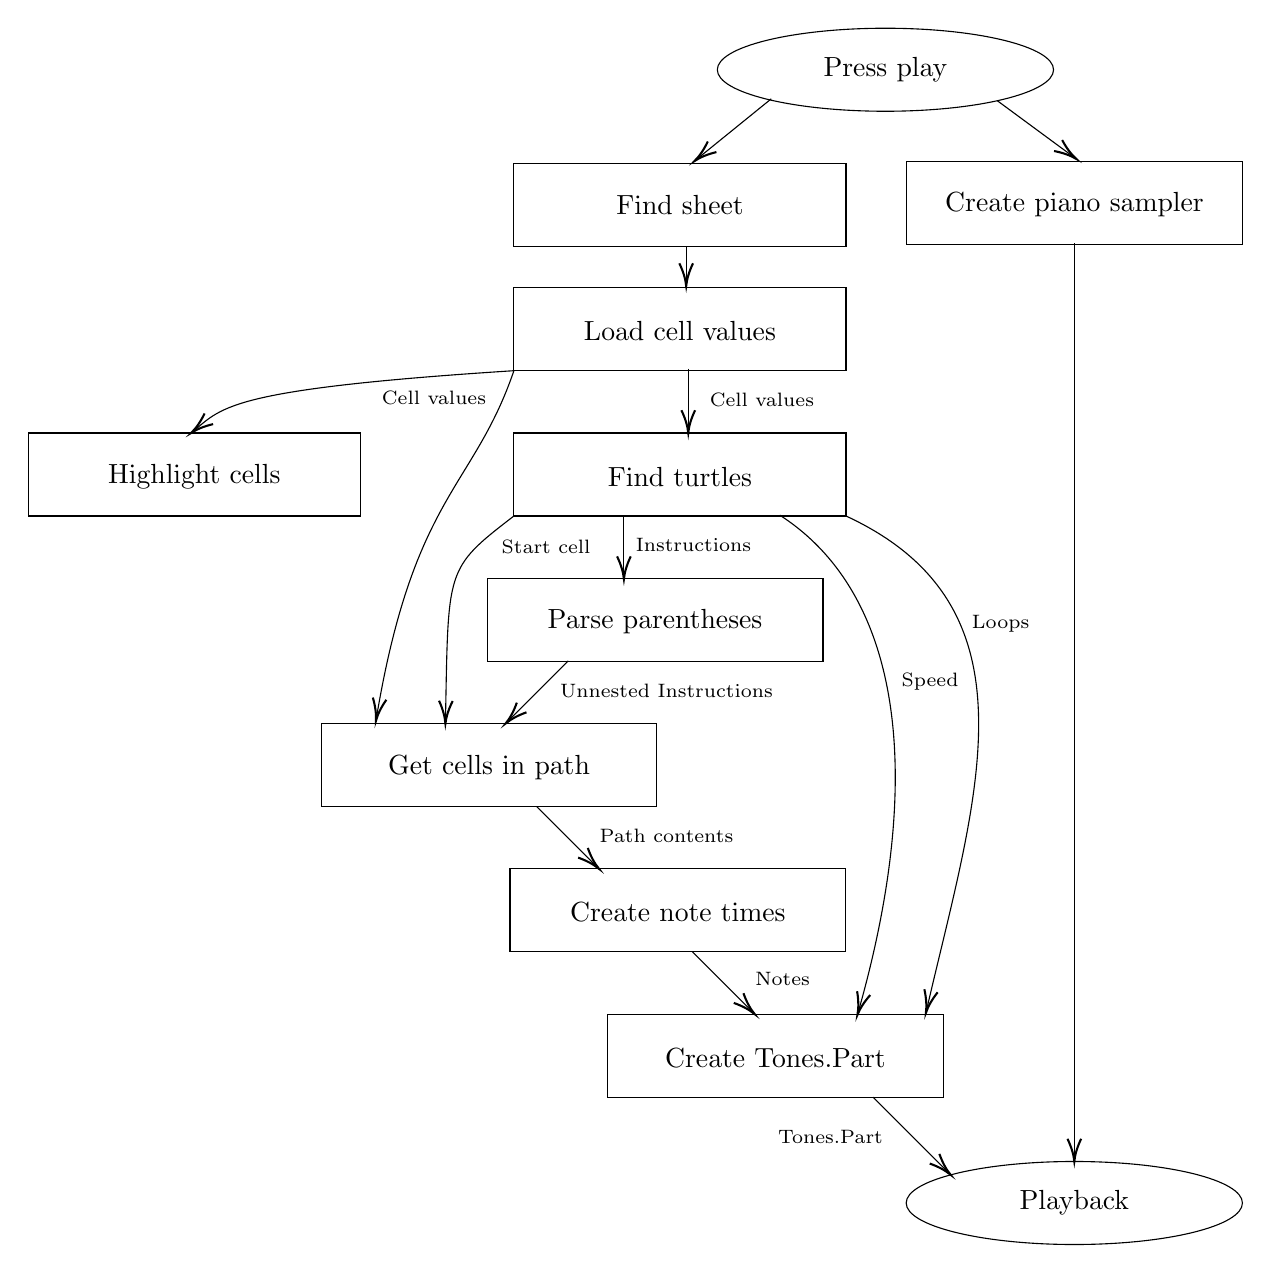
\begin{tikzpicture}[x=0.75pt,y=0.75pt,yscale=-1,xscale=1]
%uncomment if require: \path (0,604); %set diagram left start at 0, and has height of 604

%Shape: Rectangle [id:dp3390223975782729]
\draw   (244.5,71) -- (404.5,71) -- (404.5,111) -- (244.5,111) -- cycle ;

%Shape: Rectangle [id:dp7168559924493858]
\draw   (244.5,131) -- (404.5,131) -- (404.5,171) -- (244.5,171) -- cycle ;

%Shape: Rectangle [id:dp8835932361497658]
\draw   (433.7,70) -- (595.5,70) -- (595.5,110) -- (433.7,110) -- cycle ;

%Shape: Rectangle [id:dp9464422191216635]
\draw   (244.5,201) -- (404.5,201) -- (404.5,241) -- (244.5,241) -- cycle ;

%Shape: Rectangle [id:dp6384624480751633]
\draw   (231.6,271) -- (393.4,271) -- (393.4,311) -- (231.6,311) -- cycle ;

%Shape: Rectangle [id:dp2927464084046889]
\draw   (151.6,341) -- (313.4,341) -- (313.4,381) -- (151.6,381) -- cycle ;

%Shape: Rectangle [id:dp9052659554068596]
\draw   (242.6,411) -- (404.4,411) -- (404.4,451) -- (242.6,451) -- cycle ;

%Shape: Rectangle [id:dp5637329489183025]
\draw   (289.6,481) -- (451.4,481) -- (451.4,521) -- (289.6,521) -- cycle ;

%Curve Lines [id:da3917180624639185]
\draw    (244.5,241) .. controls (211.17,266.67) and (212.98,265.81) .. (211.52,339.88) ;
\draw [shift={(211.5,341)}, rotate = 271.14] [color={rgb, 255:red, 0; green, 0; blue, 0 }  ][line width=0.75]    (10.93,-3.29) .. controls (6.95,-1.4) and (3.31,-0.3) .. (0,0) .. controls (3.31,0.3) and (6.95,1.4) .. (10.93,3.29)   ;

%Straight Lines [id:da6961662223442007]
\draw    (297.5,241) -- (297.5,269.4) ;
\draw [shift={(297.5,271.4)}, rotate = 270] [color={rgb, 255:red, 0; green, 0; blue, 0 }  ][line width=0.75]    (10.93,-3.29) .. controls (6.95,-1.4) and (3.31,-0.3) .. (0,0) .. controls (3.31,0.3) and (6.95,1.4) .. (10.93,3.29)   ;

%Curve Lines [id:da9168950950169605]
\draw    (372.6,240.6) .. controls (431.31,278.41) and (442.88,365.52) .. (410.49,479.68) ;
\draw [shift={(410,481.4)}, rotate = 286.01] [color={rgb, 255:red, 0; green, 0; blue, 0 }  ][line width=0.75]    (10.93,-3.29) .. controls (6.95,-1.4) and (3.31,-0.3) .. (0,0) .. controls (3.31,0.3) and (6.95,1.4) .. (10.93,3.29)   ;

%Curve Lines [id:da7972588626438504]
\draw    (404.5,241) .. controls (499.03,284.78) and (467.32,375.49) .. (443.36,478.84) ;
\draw [shift={(443,480.4)}, rotate = 282.99] [color={rgb, 255:red, 0; green, 0; blue, 0 }  ][line width=0.75]    (10.93,-3.29) .. controls (6.95,-1.4) and (3.31,-0.3) .. (0,0) .. controls (3.31,0.3) and (6.95,1.4) .. (10.93,3.29)   ;

%Straight Lines [id:da6822022155717844]
\draw    (270.7,310.8) -- (241.91,339.59) ;
\draw [shift={(240.5,341)}, rotate = 315] [color={rgb, 255:red, 0; green, 0; blue, 0 }  ][line width=0.75]    (10.93,-3.29) .. controls (6.95,-1.4) and (3.31,-0.3) .. (0,0) .. controls (3.31,0.3) and (6.95,1.4) .. (10.93,3.29)   ;

%Straight Lines [id:da4884596231580207]
\draw    (255.5,381) -- (284.09,409.59) ;
\draw [shift={(285.5,411)}, rotate = 225] [color={rgb, 255:red, 0; green, 0; blue, 0 }  ][line width=0.75]    (10.93,-3.29) .. controls (6.95,-1.4) and (3.31,-0.3) .. (0,0) .. controls (3.31,0.3) and (6.95,1.4) .. (10.93,3.29)   ;

%Straight Lines [id:da9233366942734922]
\draw    (330.5,451) -- (359.09,479.59) ;
\draw [shift={(360.5,481)}, rotate = 225] [color={rgb, 255:red, 0; green, 0; blue, 0 }  ][line width=0.75]    (10.93,-3.29) .. controls (6.95,-1.4) and (3.31,-0.3) .. (0,0) .. controls (3.31,0.3) and (6.95,1.4) .. (10.93,3.29)   ;

%Straight Lines [id:da3670498457872964]
\draw    (417.5,521) -- (453.49,556.99) ;
\draw [shift={(454.9,558.4)}, rotate = 225] [color={rgb, 255:red, 0; green, 0; blue, 0 }  ][line width=0.75]    (10.93,-3.29) .. controls (6.95,-1.4) and (3.31,-0.3) .. (0,0) .. controls (3.31,0.3) and (6.95,1.4) .. (10.93,3.29)   ;

%Straight Lines [id:da28794703530347365]
\draw    (327.5,111) -- (327.5,128.2) ;
\draw [shift={(327.5,130.2)}, rotate = 270] [color={rgb, 255:red, 0; green, 0; blue, 0 }  ][line width=0.75]    (10.93,-3.29) .. controls (6.95,-1.4) and (3.31,-0.3) .. (0,0) .. controls (3.31,0.3) and (6.95,1.4) .. (10.93,3.29)   ;

%Straight Lines [id:da33376731250782754]
\draw    (328.5,170) -- (328.5,199) ;
\draw [shift={(328.5,201)}, rotate = 270] [color={rgb, 255:red, 0; green, 0; blue, 0 }  ][line width=0.75]    (10.93,-3.29) .. controls (6.95,-1.4) and (3.31,-0.3) .. (0,0) .. controls (3.31,0.3) and (6.95,1.4) .. (10.93,3.29)   ;

%Curve Lines [id:da2676626927985757]
\draw    (244.5,171) .. controls (225.1,227.72) and (196.29,230.77) .. (178.27,338.17) ;
\draw [shift={(178,339.8)}, rotate = 279.38] [color={rgb, 255:red, 0; green, 0; blue, 0 }  ][line width=0.75]    (10.93,-3.29) .. controls (6.95,-1.4) and (3.31,-0.3) .. (0,0) .. controls (3.31,0.3) and (6.95,1.4) .. (10.93,3.29)   ;

%Straight Lines [id:da024649031996502035]
\draw    (514.5,109.6) -- (514.5,550) ;
\draw [shift={(514.5,552)}, rotate = 270] [color={rgb, 255:red, 0; green, 0; blue, 0 }  ][line width=0.75]    (10.93,-3.29) .. controls (6.95,-1.4) and (3.31,-0.3) .. (0,0) .. controls (3.31,0.3) and (6.95,1.4) .. (10.93,3.29)   ;

%Shape: Ellipse [id:dp13505581605963868]
\draw   (433.5,572) .. controls (433.5,560.95) and (469.76,552) .. (514.5,552) .. controls (559.24,552) and (595.5,560.95) .. (595.5,572) .. controls (595.5,583.05) and (559.24,592) .. (514.5,592) .. controls (469.76,592) and (433.5,583.05) .. (433.5,572) -- cycle ;

%Shape: Ellipse [id:dp006287630832967794]
\draw   (342.5,26) .. controls (342.5,14.95) and (378.76,6) .. (423.5,6) .. controls (468.24,6) and (504.5,14.95) .. (504.5,26) .. controls (504.5,37.05) and (468.24,46) .. (423.5,46) .. controls (378.76,46) and (342.5,37.05) .. (342.5,26) -- cycle ;

%Straight Lines [id:da09048722077694915]
\draw    (368.5,40) -- (333.05,68.74) ;
\draw [shift={(331.5,70)}, rotate = 320.96000000000004] [color={rgb, 255:red, 0; green, 0; blue, 0 }  ][line width=0.75]    (10.93,-3.29) .. controls (6.95,-1.4) and (3.31,-0.3) .. (0,0) .. controls (3.31,0.3) and (6.95,1.4) .. (10.93,3.29)   ;

%Straight Lines [id:da9578993167654264]
\draw    (477.5,41) -- (513.89,67.81) ;
\draw [shift={(515.5,69)}, rotate = 216.38] [color={rgb, 255:red, 0; green, 0; blue, 0 }  ][line width=0.75]    (10.93,-3.29) .. controls (6.95,-1.4) and (3.31,-0.3) .. (0,0) .. controls (3.31,0.3) and (6.95,1.4) .. (10.93,3.29)   ;

%Shape: Rectangle [id:dp25073410390478523]
\draw   (10.5,201) -- (170.5,201) -- (170.5,241) -- (10.5,241) -- cycle ;

%Curve Lines [id:da2454539812308738]
\draw    (244.5,171) .. controls (108.92,179.69) and (104.17,188.37) .. (90.53,199.75) ;
\draw [shift={(89,201)}, rotate = 321.34000000000003] [color={rgb, 255:red, 0; green, 0; blue, 0 }  ][line width=0.75]    (10.93,-3.29) .. controls (6.95,-1.4) and (3.31,-0.3) .. (0,0) .. controls (3.31,0.3) and (6.95,1.4) .. (10.93,3.29)   ;


% Text Node
\draw (324.5,91) node  [align=left] {Find sheet};
% Text Node
\draw (324.5,152) node  [align=left] {Load cell values};
% Text Node
\draw (514.6,91) node  [align=left] {Create piano sampler};
% Text Node
\draw (324.5,222) node  [align=left] {Find turtles};
% Text Node
\draw (312.5,292) node  [align=left] {Parse parentheses};
% Text Node
\draw (232.5,362) node  [align=left] {Get cells in path};
% Text Node
\draw (323.5,432) node  [align=left] {Create note times};
% Text Node
\draw (370.5,502) node  [align=left] {Create Tones.Part};
% Text Node
\draw (514.5,572) node [] [align=left] {\textcolor[rgb]{0,0,0}{Playback}};
% Text Node
\draw (260,256) node  [align=left] {{\scriptsize Start cell}};
% Text Node
\draw (331,255) node  [align=left] {{\scriptsize Instructions}};
% Text Node
\draw (445,321) node  [align=left] {{\scriptsize Speed}};
% Text Node
\draw (479,293) node  [align=left] {{\scriptsize Loops}};
% Text Node
\draw (318,325) node  [align=left] {{\scriptsize Unnested Instructions}};
% Text Node
\draw (318,395) node  [align=left] {{\scriptsize Path contents}};
% Text Node
\draw (374,464) node  [align=left] {{\scriptsize Notes}};
% Text Node
\draw (397,540) node  [align=left] {{\scriptsize Tones.Part}};
% Text Node
\draw (206,184) node  [align=left] {{\scriptsize Cell values}};
% Text Node
\draw (423.5,26) node [] [align=left] {Press play};
% Text Node
\draw (364,185) node  [align=left] {{\scriptsize Cell values}};
% Text Node
\draw (90.5,222) node  [align=left] {Highlight cells};


\end{tikzpicture}

\end{center}

\begin{algorithm}[!htbp]
\caption{Parsing bracketed expression}\label{alg:parenthesis}
\begin{algorithmic}[1]
\Procedure{parseBrackets}{$str$}

   \State $idPadding\gets \texttt{\upquote{\_\_\_}}$
   \State $unnestedStr\gets []$
   \State $deepestLevelBracketsRE\gets \texttt{RegExp(\upquote{\textbackslash\textbackslash([\^{}\textbackslash\textbackslash(\textbackslash\textbackslash)]*\textbackslash\textbackslash)})}$
   \State $replacementIDRE\gets \texttt{RegExp(\upquote{\textbackslash\textbackslash} + }idPadding\texttt{ + \upquote{([0-9]+)} + }idPadding\texttt{)}$\\

   \Procedure{replaceDeepestBracket}{$x$}
     \State \texttt{unnestedStr.push(x.substring(1, x.length-1))}
     \State \texttt{\textbf{return} idPadding + (unnestedStr.length - 1) + idPadding}
   \EndProcedure \\

   \While{\texttt{deepestLevelBracketsRE.test(str)}}
     \State \texttt{str = str.replace(deepestLevelBracketsRE,replaceDeepestBracket)}
   \EndWhile

   \State \texttt{unnestedStr[0] = str}\\

   \Procedure{reNest}{$outerStr$}
     \State $renestingStr\gets []$
     \While{There is a match of $replacementIDRE$ in $outerStr$}
       \State $matchIndex\gets$ index of the match in $outerStr$
       \State $matchID\gets$ ID of the match (number between padding)
       \State $matchString\gets$ matched string\\

       \If{$matchIndex >$ 0}
				\State $renestingStr$.push($outestStr$.substring(0, $matchIndex$))
			\EndIf
			\State $renestingStr$.push(reNest($unnestedStr$[$firstMatchID$]))
			\State $outestStr$ = $outestStr$.substring($matchIndex$ + $matchString$.length)
     \EndWhile
     \State $renestingStr$.push($outestStr$)
     \State \textbf{return} $renestingStr$
   \EndProcedure \\

   \State \textbf{return} reNest($unnestedStr$[0])

\EndProcedure
\end{algorithmic}
\end{algorithm}

\section{Simple diagrams}

Simple diagrams can be written directly in \LaTeX.  For example, see
figure~\ref{latexpic1} on page~\pageref{latexpic1} and see
figure~\ref{latexpic2} on page~\pageref{latexpic2}.

\begin{figure}
\setlength{\unitlength}{1mm}
\begin{center}
\begin{picture}(125,100)
\put(0,80){\framebox(50,10){AAA}}
\put(0,60){\framebox(50,10){BBB}}
\put(0,40){\framebox(50,10){CCC}}
\put(0,20){\framebox(50,10){DDD}}
\put(0,00){\framebox(50,10){EEE}}

\put(75,80){\framebox(50,10){XXX}}
\put(75,60){\framebox(50,10){YYY}}
\put(75,40){\framebox(50,10){ZZZ}}

\put(25,80){\vector(0,-1){10}}
\put(25,60){\vector(0,-1){10}}
\put(25,50){\vector(0,1){10}}
\put(25,40){\vector(0,-1){10}}
\put(25,20){\vector(0,-1){10}}

\put(100,80){\vector(0,-1){10}}
\put(100,70){\vector(0,1){10}}
\put(100,60){\vector(0,-1){10}}
\put(100,50){\vector(0,1){10}}

\put(50,65){\vector(1,0){25}}
\put(75,65){\vector(-1,0){25}}
\end{picture}
\end{center}
\caption{A picture composed of boxes and vectors.}
\label{latexpic1}
\end{figure}

\begin{figure}
\setlength{\unitlength}{1mm}
\begin{center}

\begin{picture}(100,70)
\put(47,65){\circle{10}}
\put(45,64){abc}

\put(37,45){\circle{10}}
\put(37,51){\line(1,1){7}}
\put(35,44){def}

\put(57,25){\circle{10}}
\put(57,31){\line(-1,3){9}}
\put(57,31){\line(-3,2){15}}
\put(55,24){ghi}

\put(32,0){\framebox(10,10){A}}
\put(52,0){\framebox(10,10){B}}
\put(37,12){\line(0,1){26}}
\put(37,12){\line(2,1){15}}
\put(57,12){\line(0,2){6}}
\end{picture}

\end{center}
\caption{A diagram composed of circles, lines and boxes.}
\label{latexpic2}
\end{figure}



\section{Adding more complicated graphics}

The use of \LaTeX\ format can be tedious and it is often better to use
encapsulated postscript (EPS) or PDF to represent complicated graphics.
Figure~\ref{epsfig} and~\ref{xfig} on page \pageref{xfig} are
examples. The second figure was drawn using \texttt{xfig} and exported in
{\tt.eps} format. This is my recommended way of drawing all diagrams.


\begin{figure}[tbh]
\centerline{\includegraphics{figs/cuarms.pdf}}
\caption{Example figure using encapsulated postscript}
\label{epsfig}
\end{figure}

\begin{figure}[tbh]
\vspace{4in}
\caption{Example figure where a picture can be pasted in}
\label{pastedfig}
\end{figure}


\begin{figure}[tbh]
\centerline{\includegraphics{figs/diagram.pdf}}
\caption{Example diagram drawn using \texttt{xfig}}
\label{xfig}
\end{figure}


\chapter{Implementation}

In this chapter I shall first explain how the turtles, using the movement instructions defined previously, are defined and controlled. The remaining features in the initial prototype will be explained. The format and results of the formative evaluation using this initial prototype shall be summarised. I shall then cover the design decisions and changes that were made to the Excello prototype during the participatory design process. Then, how Excello has been implemented will be described followed by the MIDI to Excello converter. The chapter concludes with an overview of the project repository.

\section{Initial Prototype}

Notes and turtles can be defined in any cell in the spreadsheet. When the Excello add-in is opened, a window will open in the right side of Excel. This contains a play and stop button which can be used to launch all the turtles defined in the spreadsheet and initiate playback. Playback is a realistic piano sound.

A summary of the musical elements that can be put in cells and that will be interpreted by turtles is shown in table \ref{tab:cells}

\begin{table}
\centering
% \caption{Grammar Rules for the turtle movement instructions. $z \in \Z$}
\caption{Definition of notes in cells.}
\begin{tabular}{|l|l|} \hline
\textbf{Interpretation}&\textbf{Format}\\ \hline
Note& Note name (A-G), optional accidentals and octave \\
&number e.g. \texttt{F\#4}\\ \hline
Sustain& \texttt{s}\\ \hline
Multiple notes& Notes, rests or sustains separated by a comma. Rests \\
subdivided in time& must be a space or an empty string e.g. \texttt{E4,,C4,s}\\ \hline
Rest& Any cell not interpreted as a note, sustain or multi-note. \\ \hline
\end{tabular}
\label{tab:cells}
\end{table}

\subsection{Turtles}

Notes are played by defining and launching turtles to navigate the spreadsheet. Turtles are defined as follows:

\texttt{!turtle(<Starting Cell>, <Movement>, <Speed>, <Number of Loops>)}

\subsubsection{Activation}

The "\texttt{!}" dictates that the turtle will be activated when the play button in the add-in window is pressed. Just like many digital audio workstations allow muting and soloing of tracks, this can be used to quickly modify which turtles will play without losing the definition of the turtle.

\subsubsection{Starting Cell}

The starting cell of the turtle is given by the cell reference. As with conventional Excel formulae, columns are defined in base 26 using the letters of the alphabet and rows are numbered using the integers. A cell is defined by the concatenation of the column letters and row number. This cell will be played and is the first cell in the path of the turtle.

As each turtle only plays one note at a time, multiple turtles must be defined to play polyphonic music such as chords. It was believed that in these cases the turtles may follow identical paths but in adjacent rows or columns. Multiple turtles following identical paths but starting from adjacent cells can be defined using the existing Excel range notation to define the starting cells. "\texttt{A2:A5}" would define four turtles in the cells A2,A3,A4,A5. This prevents the writing of multiple turtle definitions differing in only the start cell row.

\subsubsection{Movement}

The turtles start facing north. The design of the language used to define turtle movement has been discussed in the preparation chapter. Using brackets to repeat multiple instructions within the turtle's instructions was not implemented by the start of the participatory design process.

\subsubsection{Speed}

An optional third argument can be provided to defined the speed at which the turtle moves through the grid. If the argument is not provided, the turtle moves at 160 cells per minute through the grid. The speed argument defines the speed relative to 160 cells per minute. Therefore if the argument "\texttt{2}" was provided, this would move through the grid at 320 cells per minute. This relative system was used so it would be easier to tell the speed relation between two turtles. This would be particularly beneficial for phase music. Arbitrary maths can be provided for this argument and it will be evaluated. This can be used to define a turtle  speed is an irrational multiple of another's.

\subsubsection{Number of Loops}

An optional fourth argument defines the number of times the path of the turtle is played. If committed the turtle will loop infinitely. This was included so that repeating parts (e.g. the cello part of Pachabel's Canon in D) need only defining once but can be played repetitively.

\subsection{Highlighting}

In order to assist in the recognition of notes and turtles, when the play button is pressed, cells are highlighted depending on their contents. Cells containing activated or deactivated definitions of turtles are highlighted green. Cells containing definitions of notes, or multiple notes, are highlighted red, with cells only containing a sustain highlighted a lighter red, to show a correspondance to notes whilst not carrying quite so much information.

\subsection{Chord input}

In order to maintain musical abstractions of chords and arpeggios \footnote{Where the notes of a chord are played in rising or descending order} whilst keeping to paradigm of a turtle being responsible for up to one note at any time, a tool to add chords and arpeggios is available. The note, type (over 100 available), inversion and starting octave of the chord are inputted in four drop-down selectors and the notes making up that chord are entered into the grid using the insert button. If a single cell or range taller than it is wide is highlighted in the spreadsheet, the notes will be inserted in adjacent vertical cells starting at the top-left of the range. Otherwise, the notes will be inserted horizontally. This means whether the turtles are moving horizontally or vertically both chords and arpeggios can be easily defined. As a result, helpful musical abstractions are still available whilst keeping the cleanness of the turtle system.

\section{Formative Evaluation}

In order to guide the development of the project to best suite the users, participants were involved in formative evaluation. 21 participants took place in the participatory design process. Participants were all University of Cambridge students, across a range of subjects, but all musical. Initially, individual meetings were held with each participant. A tutorial of the initial prototype was given followed by the carrying out of a short exercise lasting 15-20 minutes in most cases. After both the tutorial and the exercise, users were asked to comment on how they found Excello. Particular attention was drawn to actions that they found particularly unintuitive or required notable mental effort. Comparisons were also made to the musical interfaces that participants were already familiar with. The sessions were audio recorded in order to prevent the jotting down of notes causing delays, and later notes were made from these recordings. The ethical and data handling procedures that were carried out shall be discussed in the evaluation chapter.

In order to simulate the most likely ways in which Excello would be used, participants were given the freedom to carry out an exercise of their choice. In many cases this was transcribing an exiting piece from memory or from traditional western notation into the Excello notation. Two tasks were provided to choose from if participants had no immediate inspiration. These were to transcribe a piece of music from western notation or to make changes to an existing piece in the Excello notation.

These sessions were carried out at the beginning of Lent term 2019. Participants were asked if they would be willing to continue using Excello personally from their initial session until the summative evaluation sessions, eight weeks later. This gave time for additional feedback to be given as participants used Excello in their own time. It also ensured that the summative evaluation carried out would be done so by users with sufficient experience of the interface. Participants were encouraged to get in contact with any additional issues or suggestions they had during this time.

\subsection{Issues and Suggestions}

The issues and suggestions that arose during the participatory design period have been categorised and summarised below.

\subsubsection{Turtle Notation}

Having dynamic instructions within the turtle was found to make it harder to extract the path that the turtle followed as not all instructions related to the way in which the turtle moves. As the dynamics weren't next to the notes they corresponded to, it was challenging to establish which volume a given note would be played at or where to place the dynamic instructions within the turtle to correspond to a certain note positioned elsewhere in the spreadsheet. In the initial prototype there was no way to assign a dynamic to the first note without having the starting cell being empty. The addition of this empty cell could be inconvenient for looping parts as this empty cell would be included in the loop. Users who were not familiar with the dynamic markings of western notation found them unintuitive. Furthermore, it was noted that these discrete markings do not make available the continuous volume scale that could be possible with the interface.

When trying to transcribe a piece in an exact tempo, having to divide the speed by 160 in order to enter a relative speed caused unnecessary work. There was forgetfulness as to the whether relative speed referred to how long or how quickly the turtle moved.

Having completed the tutorial, users often has to check which arguments appeared where within the turtle definition or what the arguments were.

When parsing the instruction, as the number of dynamics and movement instructions grew and the instruction became long, it could become quite tough to establish how the turtle would behave. As "\texttt{s}" could be used to indicate sustain within cells, some users confused the "\texttt{s}" within the turtle instructions to mean sustain and not south.

\subsubsection{Feedback}

Having clicked the play button it was often not clear if this had been registered. Especially if the Excel workbook was saving, and this caused a delay in Excello being able to access the spreadsheet. It was also requested if it would be possible to see a summary of where the active turtle were in addition to them being highlighted green. If a turtle had accidentally been left activated, the entire grid had to be searched in order to locate it.

\subsubsection{MIDI conversions}

Many users, especially those who used production software such as GarageBand and Logic, said that it would be helpful to be able to interact with MIDI files. Being able to use Excello to create their chord sequences and bass lines before adding additional effects and recorded lines in their digital audio work stations would require a MIDI export. In addition, if working with an existing MIDI file, it would be convenient to be able to convert that into the Excello notation.

\subsubsection{Sources of effort when writing}

Once notes had been inputted into the grid, often in a single straight line, the number of cells had to be counted so the turtle could be moved the correct number of cells. Whilst Excel allows users to highlight a selection of cells and have an immediate output of how many cells are highlighted without any formula being written, this is still an unproductive use of time. Some users would simply instruct the turtle to move forward significantly more steps than required to prevent this counting, but this is not feasible for looping parts. It was suggested that turtles could figure out how far they should move so that the instruction didn't need editing when more notes were added. This was particularly inconvenient when users were writing out a piece and periodically testing what they had written so far.

If instructions involved repeats such as repeatedly moving to the end of a line and jumping down a few cells and back to the beginning of the line, instructions within the turtles required a lot of repetition.

If writing out a melodic line consisting of small movements, many of the notes would take place in the same octave. As such, it was tiresome to have to repeatedly write out the octave number when this was barely changing. One user made a comparison to LilyPond \footnote{A program for music notation using text notation.} \cite{sandberg:lily} where if the length of a note is not defined, the last defined note length would be used.

Some users said they would find it more intuitive to think of a melodic line in terms of the intervals between notes as opposed to the name of each note. If a piece contained a melodic line that was modulated \footnote{Where every note has been moved up or down in pitch by the same amount.}, the modulated part had to be written out again and could not be derived quicker from the original version.

\subsubsection{Chords}

Whilst the variety of available chord types was appreciated, most users used a very small subset of these but still had to scroll through the whole list to find these. Separating the more common chords for easier access was requested. In the initial prototype, the notes were inserted from low to high. This meant that notes inserted in a vertical line had the lowest note at the top with notes increasing in pitch proceeding down the column. In western staff notation, higher pitch notes appear higher up the staff. As a result, it was suggested that inverting the order would be more intuitive. In the initial interface it was also unclear what the different drop downs corresponded to, with some users selecting the "7" from the octave number in order to try and insert a Maj7 chord.

\subsubsection{Activation of turtles}

When toggling the activation of a turtle, it was very tedious to have to enter the edit mode for each cell containing a turtle definition and add or remove the exclamation mark. This was particularly so if a piece had multiple turtle definitions.

\section{Second Prototype}

Following the formative evaluation sessions carried out with the participants and the feedback that was received, a series of additions and modifications were made to the prototype to solve the problems and opportunities brought up.

\subsection{Dynamics}

In order to assist users in extracting the path that the turtles follow from the instructions and pairing notes with their volume, dynamics are instead inserted in the cells along with the notes. A dynamic instruction is added after the note, separated by a space as in Manhattan \cite{nash:manhattan}. As before, this will persist for all following notes until the volume is redefined. By moving the dynamics into the cell there is a tradeoff. A single turtle definition with multiple start cells can now play parts of different volume. However, notes in the grid are limited to only being played at the given volume. To play the same notes at a different volume would require a different path to be followed by the turtle where the cells defining the volume are missed and other cells are played. Overall, the new system was believed to be more preferable.

In order to be able to make use of a full continuous dynamic scale, in addition to the existing dynamic symbols available, a number between 0 and 1 can be provided where 0 will be silent and 1 is equivalent to fff.

\subsection{Nested Instructions}

The initial language design included the use of nested instruction in order to allow for easy repetition of turtle movements. This was not implemented when the first formative evaluation sessions took place. However, this should help reduce the length of turtle instructions and allow for repeated sections or movements to be more easily incorporated. A series of instructions placed within parentheses with a number immediately following the closing parenthesis will be repeated that number of times. Whilst the fourth argument of the turtle will simply repeat the musical output of the turtle, repetitions within the turtle instruction allow paths to be defined more concisely.

\subsection{Absolute Tempo}

The speed at which the turtle moves is now defined by cells per minute, rather than the relative value used initially. However, values less than 10 were interpreted in the original relative way to maintain backwards compatibility for the participant's existing work. To maintain consistency in a production version, this would be removed so speed must be defined absolutely. This also ensures that the values given for speed and dynamics will be of different orders of magnitude and hence reduce the confusion that can occur between them.

\subsection{Custom Excel Functions}

Two custom Excel functions were implemented to aid in the composition of music within Excel. One to aid with inserting turtles into the grid and a second to transpose notes.

\subsubsection{Excello.Turtle}

Many users had commented they forgot which arguments go where within the turtle. By adding custom Excel functions the existing formulae writing tools provided within Excel can be utilised. When using a built in formula, a prompt appears informing users which arguments go where and whether they are optional. The output of this function is text used to define a turtle if written manually. This also allows other cells to be referenced for the arguments of the turtle function. For example a cell could have speed defined that all other turtles reference. As a result, the speed of all turtles could be modified by changing this single value. This also allows relative tempos to be easily implemented again as the speed argument of the turtle could be defined as a relative speed mutliplied by the global speed (given as a cell referece).

\subsubsection{Excello.Modulate}

The implementation of a function to modulate notes both allows for the easy modulation of existing sections of a piece and also the definition of a melodic line by the intervals between the notes. The function takes the contents of a cell where a note is defined and an interval and outputs the note transposed by that interval. A section can be modulated by calling this function on the first note with a provided interval and using the existing drag-fill functionality of Excel to modulate all notes. By using the previous note that has just been transposed and one of a series of intervals as the arguments, a melodic line can quickly be produced from a starting note and a series of intervals.

%  \ref{examples}

\subsection{Sustain}

In order to prevent confusion between the instruction for a turtle to face south and for a note to be sustained. The symbol "\texttt{-}" has been chosen to sustain a note. This was chosen because it is light and also has some similarity to a tie \footnote{A line to increase the length of a note by joining to another.}. The use of an "\texttt{s}" is still interpreted as a sustain to maintain backwards compatibility for the existing work of the participants.

\subsection{Active Turtles}

In order to provide feedback that turtle definitions have been recognised, in addition to green highlighting, a list of the active turtles is given below the play button. This also assists in finding any spurious turtles that were not intended to be activated.

\subsection{Automatic Movement}

To prevent the number of cells in a line needing counting, a turtle can be instructed to move as far as there are notes defined in the direction it is currently facing. This means that if more notes are added on this line, the turtle instructions do not need editing before pressing play. There may be cases where a part is meant to finish with a number of rests. As a rest is notated with a blank cell, a method of increasing the length of the path to include these rests is required. A rest can be given explicitly with a "\texttt{.}" allowing the distance distance travelled by the turtle when moving automatically to be increased. This would be required if multiple turtles were defining a repeating section where one does not have the final cell of the section being a note, sustain or multi-note cell. Without an explicit rest the turtle would stop and repeat too soon and the parts would be out of phase.

\subsection{Inferred Octave}

To prevent the octave number needing writing every time a note in defined, the octave number can be inferred by the program if it is omitted. There were two methods under consideration. Firstly, given that most intervals within music are small, the nearest note could be inferred. This means that a scale would only need the octave defining in the first note. Whilst this method would likely require the least explicit statement of octave number it would be non-trivial to figure out the octave a given note is played in. The last defined octave in the path would need finding and then the subsequent notes would have to be walked through keeping track of which octave is being played. The second consideration was to always use the last defined octave. Whilst this may require reasonable octave definition around the boundary between octaves, it is easier to find what octave a note is played at as it is simply the last defined octave in the path.

\subsection{Chords}

In order to assist in the entering of common chords, common chord types are repeated in a separate group  at the top of the type selection drop-down. The layout of the chord drop-downs was improved with labels added to make it clearer what the different values would refer to. If the notes were entered vertically, the order was reversed to have a greater correspondence with traditional staff notation.

\subsection{Activation of turtles}

A "Toggle Activation" button was added to the add-in window. When a cell or range is highlighted in the spreadsheet, the activation of any turtle definitions in this range will be toggled when the button is pressed.  This significantly increases the ease with which turtles can be deselected as only two clicks are required as opposed to having to enter the cell edit mode and add or remove an exclamation mark.

\section{How it works}

\section{MIDI Converter}

\section{Repository Overview}

% \section{Verbatim text}
%
% Verbatim text can be included using \verb|\begin{verbatim}| and
% \verb|\end{verbatim}|. I normally use a slightly smaller font and
% often squeeze the lines a little closer together, as in:
%
% {\renewcommand{\baselinestretch}{0.8}\small
% \begin{verbatim}
%   export function parseBrackets(str: string) {
%
%   	var unnestedStr = ['will become highest level'];
%   	var idPadding = '__';
%   	var deepestLevelBracketsRE = new RegExp('\\([^\\(\\)]*\\)');
%
%   	while (deepestLevelBracketsRE.test(str)) {
%   		str = str.replace(deepestLevelBracketsRE,function(x) {
%   			unnestedStr.push(x.substring(1, x.length-1));
%   			return idPadding + (unnestedStr.length - 1) + idPadding;
%   		});
%   	}
%   	unnestedStr[0] = str;
%
%   	var replacementIDRE = new RegExp('\\' + idPadding + '([0-9]+)' + idPadding);
%
%   	// transform references to tree
%   	function reNest (outestStr: string) {
%   		var renestingStr = [];
%   		var match;
%
%   		while (match = replacementIDRE.exec(outestStr)) {
%
%   			var matchIndex = match.index;
%   			var firstMatchID = match[1];
%   			var fullStringMatched = match[0];
%
%   			// push what was before
%   			if (matchIndex > 0) {
%   				renestingStr.push(outestStr.substring(0, matchIndex))
%   			}
%   			//perform recursively
%   			renestingStr.push(reNest(unnestedStr[firstMatchID]))
%   			// remove the string that has been processed
%   			outestStr = outestStr.substring(matchIndex + fullStringMatched.length)
%   		}
%   		renestingStr.push(outestStr)
%   		return renestingStr
%   	}
%
%   	return reNest(unnestedStr[0])
%   }
% \end{verbatim}
% }

\begin{center}


\tikzset{every picture/.style={line width=0.75pt}} %set default line width to 0.75pt

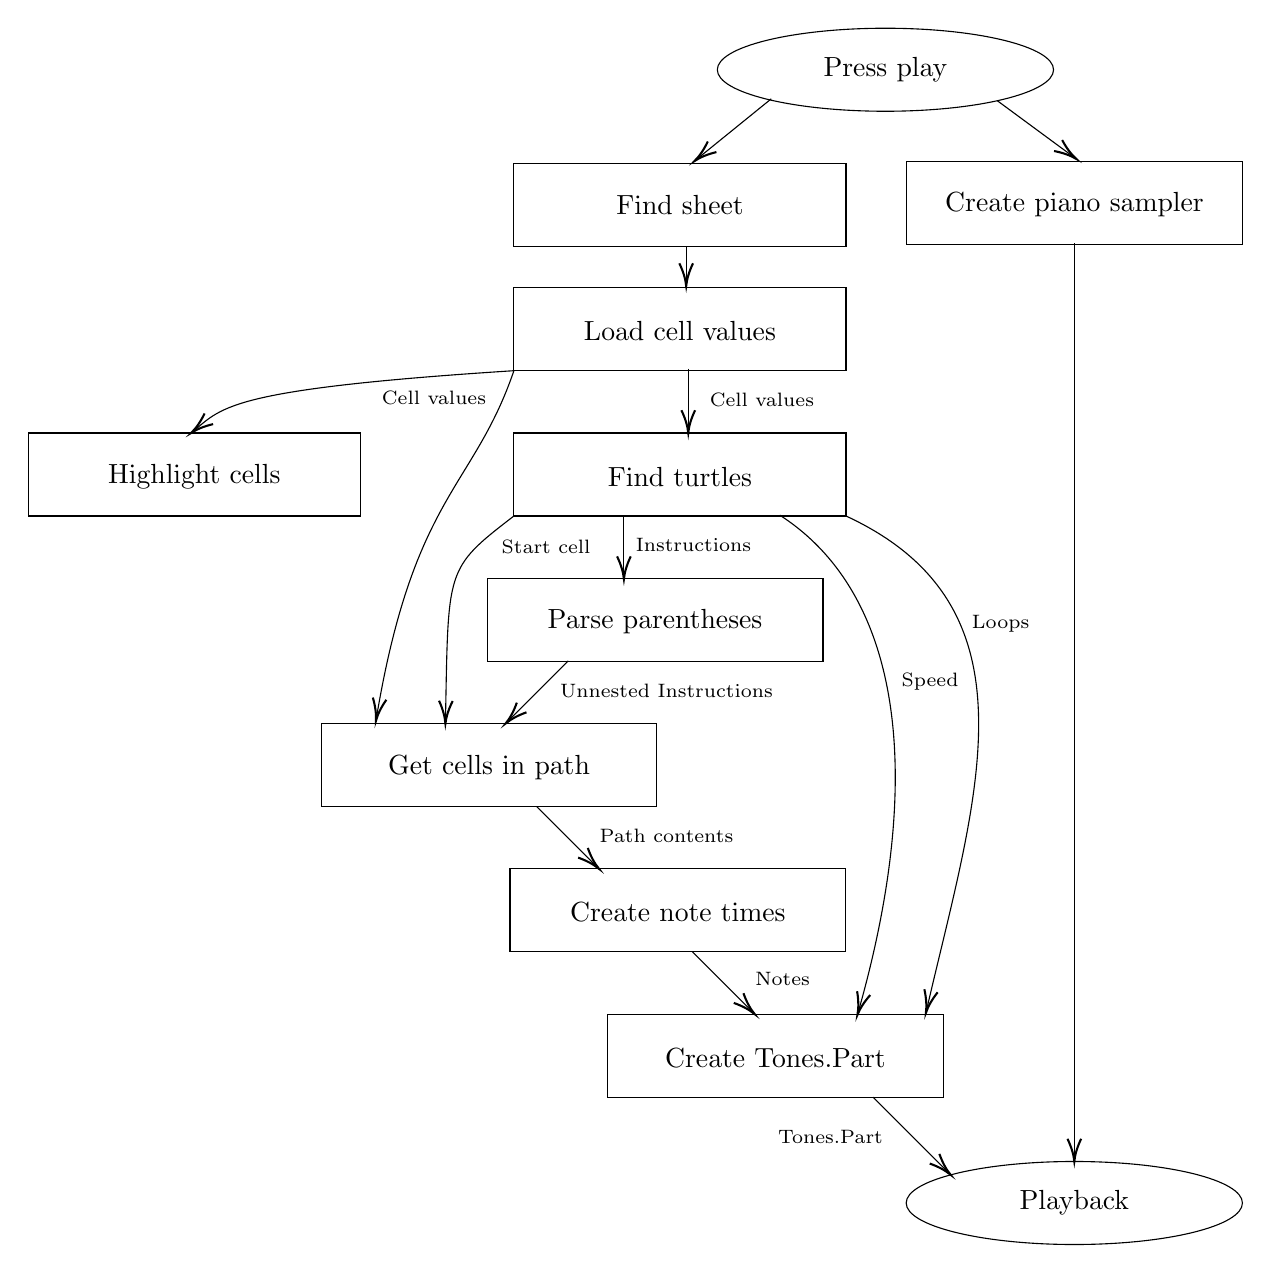
\begin{tikzpicture}[x=0.75pt,y=0.75pt,yscale=-1,xscale=1]
%uncomment if require: \path (0,604); %set diagram left start at 0, and has height of 604

%Shape: Rectangle [id:dp3390223975782729]
\draw   (244.5,71) -- (404.5,71) -- (404.5,111) -- (244.5,111) -- cycle ;

%Shape: Rectangle [id:dp7168559924493858]
\draw   (244.5,131) -- (404.5,131) -- (404.5,171) -- (244.5,171) -- cycle ;

%Shape: Rectangle [id:dp8835932361497658]
\draw   (433.7,70) -- (595.5,70) -- (595.5,110) -- (433.7,110) -- cycle ;

%Shape: Rectangle [id:dp9464422191216635]
\draw   (244.5,201) -- (404.5,201) -- (404.5,241) -- (244.5,241) -- cycle ;

%Shape: Rectangle [id:dp6384624480751633]
\draw   (231.6,271) -- (393.4,271) -- (393.4,311) -- (231.6,311) -- cycle ;

%Shape: Rectangle [id:dp2927464084046889]
\draw   (151.6,341) -- (313.4,341) -- (313.4,381) -- (151.6,381) -- cycle ;

%Shape: Rectangle [id:dp9052659554068596]
\draw   (242.6,411) -- (404.4,411) -- (404.4,451) -- (242.6,451) -- cycle ;

%Shape: Rectangle [id:dp5637329489183025]
\draw   (289.6,481) -- (451.4,481) -- (451.4,521) -- (289.6,521) -- cycle ;

%Curve Lines [id:da3917180624639185]
\draw    (244.5,241) .. controls (211.17,266.67) and (212.98,265.81) .. (211.52,339.88) ;
\draw [shift={(211.5,341)}, rotate = 271.14] [color={rgb, 255:red, 0; green, 0; blue, 0 }  ][line width=0.75]    (10.93,-3.29) .. controls (6.95,-1.4) and (3.31,-0.3) .. (0,0) .. controls (3.31,0.3) and (6.95,1.4) .. (10.93,3.29)   ;

%Straight Lines [id:da6961662223442007]
\draw    (297.5,241) -- (297.5,269.4) ;
\draw [shift={(297.5,271.4)}, rotate = 270] [color={rgb, 255:red, 0; green, 0; blue, 0 }  ][line width=0.75]    (10.93,-3.29) .. controls (6.95,-1.4) and (3.31,-0.3) .. (0,0) .. controls (3.31,0.3) and (6.95,1.4) .. (10.93,3.29)   ;

%Curve Lines [id:da9168950950169605]
\draw    (372.6,240.6) .. controls (431.31,278.41) and (442.88,365.52) .. (410.49,479.68) ;
\draw [shift={(410,481.4)}, rotate = 286.01] [color={rgb, 255:red, 0; green, 0; blue, 0 }  ][line width=0.75]    (10.93,-3.29) .. controls (6.95,-1.4) and (3.31,-0.3) .. (0,0) .. controls (3.31,0.3) and (6.95,1.4) .. (10.93,3.29)   ;

%Curve Lines [id:da7972588626438504]
\draw    (404.5,241) .. controls (499.03,284.78) and (467.32,375.49) .. (443.36,478.84) ;
\draw [shift={(443,480.4)}, rotate = 282.99] [color={rgb, 255:red, 0; green, 0; blue, 0 }  ][line width=0.75]    (10.93,-3.29) .. controls (6.95,-1.4) and (3.31,-0.3) .. (0,0) .. controls (3.31,0.3) and (6.95,1.4) .. (10.93,3.29)   ;

%Straight Lines [id:da6822022155717844]
\draw    (270.7,310.8) -- (241.91,339.59) ;
\draw [shift={(240.5,341)}, rotate = 315] [color={rgb, 255:red, 0; green, 0; blue, 0 }  ][line width=0.75]    (10.93,-3.29) .. controls (6.95,-1.4) and (3.31,-0.3) .. (0,0) .. controls (3.31,0.3) and (6.95,1.4) .. (10.93,3.29)   ;

%Straight Lines [id:da4884596231580207]
\draw    (255.5,381) -- (284.09,409.59) ;
\draw [shift={(285.5,411)}, rotate = 225] [color={rgb, 255:red, 0; green, 0; blue, 0 }  ][line width=0.75]    (10.93,-3.29) .. controls (6.95,-1.4) and (3.31,-0.3) .. (0,0) .. controls (3.31,0.3) and (6.95,1.4) .. (10.93,3.29)   ;

%Straight Lines [id:da9233366942734922]
\draw    (330.5,451) -- (359.09,479.59) ;
\draw [shift={(360.5,481)}, rotate = 225] [color={rgb, 255:red, 0; green, 0; blue, 0 }  ][line width=0.75]    (10.93,-3.29) .. controls (6.95,-1.4) and (3.31,-0.3) .. (0,0) .. controls (3.31,0.3) and (6.95,1.4) .. (10.93,3.29)   ;

%Straight Lines [id:da3670498457872964]
\draw    (417.5,521) -- (453.49,556.99) ;
\draw [shift={(454.9,558.4)}, rotate = 225] [color={rgb, 255:red, 0; green, 0; blue, 0 }  ][line width=0.75]    (10.93,-3.29) .. controls (6.95,-1.4) and (3.31,-0.3) .. (0,0) .. controls (3.31,0.3) and (6.95,1.4) .. (10.93,3.29)   ;

%Straight Lines [id:da28794703530347365]
\draw    (327.5,111) -- (327.5,128.2) ;
\draw [shift={(327.5,130.2)}, rotate = 270] [color={rgb, 255:red, 0; green, 0; blue, 0 }  ][line width=0.75]    (10.93,-3.29) .. controls (6.95,-1.4) and (3.31,-0.3) .. (0,0) .. controls (3.31,0.3) and (6.95,1.4) .. (10.93,3.29)   ;

%Straight Lines [id:da33376731250782754]
\draw    (328.5,170) -- (328.5,199) ;
\draw [shift={(328.5,201)}, rotate = 270] [color={rgb, 255:red, 0; green, 0; blue, 0 }  ][line width=0.75]    (10.93,-3.29) .. controls (6.95,-1.4) and (3.31,-0.3) .. (0,0) .. controls (3.31,0.3) and (6.95,1.4) .. (10.93,3.29)   ;

%Curve Lines [id:da2676626927985757]
\draw    (244.5,171) .. controls (225.1,227.72) and (196.29,230.77) .. (178.27,338.17) ;
\draw [shift={(178,339.8)}, rotate = 279.38] [color={rgb, 255:red, 0; green, 0; blue, 0 }  ][line width=0.75]    (10.93,-3.29) .. controls (6.95,-1.4) and (3.31,-0.3) .. (0,0) .. controls (3.31,0.3) and (6.95,1.4) .. (10.93,3.29)   ;

%Straight Lines [id:da024649031996502035]
\draw    (514.5,109.6) -- (514.5,550) ;
\draw [shift={(514.5,552)}, rotate = 270] [color={rgb, 255:red, 0; green, 0; blue, 0 }  ][line width=0.75]    (10.93,-3.29) .. controls (6.95,-1.4) and (3.31,-0.3) .. (0,0) .. controls (3.31,0.3) and (6.95,1.4) .. (10.93,3.29)   ;

%Shape: Ellipse [id:dp13505581605963868]
\draw   (433.5,572) .. controls (433.5,560.95) and (469.76,552) .. (514.5,552) .. controls (559.24,552) and (595.5,560.95) .. (595.5,572) .. controls (595.5,583.05) and (559.24,592) .. (514.5,592) .. controls (469.76,592) and (433.5,583.05) .. (433.5,572) -- cycle ;

%Shape: Ellipse [id:dp006287630832967794]
\draw   (342.5,26) .. controls (342.5,14.95) and (378.76,6) .. (423.5,6) .. controls (468.24,6) and (504.5,14.95) .. (504.5,26) .. controls (504.5,37.05) and (468.24,46) .. (423.5,46) .. controls (378.76,46) and (342.5,37.05) .. (342.5,26) -- cycle ;

%Straight Lines [id:da09048722077694915]
\draw    (368.5,40) -- (333.05,68.74) ;
\draw [shift={(331.5,70)}, rotate = 320.96000000000004] [color={rgb, 255:red, 0; green, 0; blue, 0 }  ][line width=0.75]    (10.93,-3.29) .. controls (6.95,-1.4) and (3.31,-0.3) .. (0,0) .. controls (3.31,0.3) and (6.95,1.4) .. (10.93,3.29)   ;

%Straight Lines [id:da9578993167654264]
\draw    (477.5,41) -- (513.89,67.81) ;
\draw [shift={(515.5,69)}, rotate = 216.38] [color={rgb, 255:red, 0; green, 0; blue, 0 }  ][line width=0.75]    (10.93,-3.29) .. controls (6.95,-1.4) and (3.31,-0.3) .. (0,0) .. controls (3.31,0.3) and (6.95,1.4) .. (10.93,3.29)   ;

%Shape: Rectangle [id:dp25073410390478523]
\draw   (10.5,201) -- (170.5,201) -- (170.5,241) -- (10.5,241) -- cycle ;

%Curve Lines [id:da2454539812308738]
\draw    (244.5,171) .. controls (108.92,179.69) and (104.17,188.37) .. (90.53,199.75) ;
\draw [shift={(89,201)}, rotate = 321.34000000000003] [color={rgb, 255:red, 0; green, 0; blue, 0 }  ][line width=0.75]    (10.93,-3.29) .. controls (6.95,-1.4) and (3.31,-0.3) .. (0,0) .. controls (3.31,0.3) and (6.95,1.4) .. (10.93,3.29)   ;


% Text Node
\draw (324.5,91) node  [align=left] {Find sheet};
% Text Node
\draw (324.5,152) node  [align=left] {Load cell values};
% Text Node
\draw (514.6,91) node  [align=left] {Create piano sampler};
% Text Node
\draw (324.5,222) node  [align=left] {Find turtles};
% Text Node
\draw (312.5,292) node  [align=left] {Parse parentheses};
% Text Node
\draw (232.5,362) node  [align=left] {Get cells in path};
% Text Node
\draw (323.5,432) node  [align=left] {Create note times};
% Text Node
\draw (370.5,502) node  [align=left] {Create Tones.Part};
% Text Node
\draw (514.5,572) node [] [align=left] {\textcolor[rgb]{0,0,0}{Playback}};
% Text Node
\draw (260,256) node  [align=left] {{\scriptsize Start cell}};
% Text Node
\draw (331,255) node  [align=left] {{\scriptsize Instructions}};
% Text Node
\draw (445,321) node  [align=left] {{\scriptsize Speed}};
% Text Node
\draw (479,293) node  [align=left] {{\scriptsize Loops}};
% Text Node
\draw (318,325) node  [align=left] {{\scriptsize Unnested Instructions}};
% Text Node
\draw (318,395) node  [align=left] {{\scriptsize Path contents}};
% Text Node
\draw (374,464) node  [align=left] {{\scriptsize Notes}};
% Text Node
\draw (397,540) node  [align=left] {{\scriptsize Tones.Part}};
% Text Node
\draw (206,184) node  [align=left] {{\scriptsize Cell values}};
% Text Node
\draw (423.5,26) node [] [align=left] {Press play};
% Text Node
\draw (364,185) node  [align=left] {{\scriptsize Cell values}};
% Text Node
\draw (90.5,222) node  [align=left] {Highlight cells};


\end{tikzpicture}

\end{center}

\begin{algorithm}[!htbp]
\caption{Parsing bracketed expression}\label{alg:parenthesis}
\begin{algorithmic}[1]
\Procedure{parseBrackets}{$str$}

   \State $idPadding\gets \texttt{\upquote{\_\_\_}}$
   \State $unnestedStr\gets []$
   \State $deepestLevelBracketsRE\gets \texttt{RegExp(\upquote{\textbackslash\textbackslash([\^{}\textbackslash\textbackslash(\textbackslash\textbackslash)]*\textbackslash\textbackslash)})}$
   \State $replacementIDRE\gets \texttt{RegExp(\upquote{\textbackslash\textbackslash} + }idPadding\texttt{ + \upquote{([0-9]+)} + }idPadding\texttt{)}$\\

   \Procedure{replaceDeepestBracket}{$x$}
     \State \texttt{unnestedStr.push(x.substring(1, x.length-1))}
     \State \texttt{\textbf{return} idPadding + (unnestedStr.length - 1) + idPadding}
   \EndProcedure \\

   \While{\texttt{deepestLevelBracketsRE.test(str)}}
     \State \texttt{str = str.replace(deepestLevelBracketsRE,replaceDeepestBracket)}
   \EndWhile

   \State \texttt{unnestedStr[0] = str}\\

   \Procedure{reNest}{$outerStr$}
     \State $renestingStr\gets []$
     \While{There is a match of $replacementIDRE$ in $outerStr$}
       \State $matchIndex\gets$ index of the match in $outerStr$
       \State $matchID\gets$ ID of the match (number between padding)
       \State $matchString\gets$ matched string\\

       \If{$matchIndex >$ 0}
				\State $renestingStr$.push($outestStr$.substring(0, $matchIndex$))
			\EndIf
			\State $renestingStr$.push(reNest($unnestedStr$[$firstMatchID$]))
			\State $outestStr$ = $outestStr$.substring($matchIndex$ + $matchString$.length)
     \EndWhile
     \State $renestingStr$.push($outestStr$)
     \State \textbf{return} $renestingStr$
   \EndProcedure \\

   \State \textbf{return} reNest($unnestedStr$[0])

\EndProcedure
\end{algorithmic}
\end{algorithm}

\section{Simple diagrams}

Simple diagrams can be written directly in \LaTeX.  For example, see
figure~\ref{latexpic1} on page~\pageref{latexpic1} and see
figure~\ref{latexpic2} on page~\pageref{latexpic2}.

\begin{figure}
\setlength{\unitlength}{1mm}
\begin{center}
\begin{picture}(125,100)
\put(0,80){\framebox(50,10){AAA}}
\put(0,60){\framebox(50,10){BBB}}
\put(0,40){\framebox(50,10){CCC}}
\put(0,20){\framebox(50,10){DDD}}
\put(0,00){\framebox(50,10){EEE}}

\put(75,80){\framebox(50,10){XXX}}
\put(75,60){\framebox(50,10){YYY}}
\put(75,40){\framebox(50,10){ZZZ}}

\put(25,80){\vector(0,-1){10}}
\put(25,60){\vector(0,-1){10}}
\put(25,50){\vector(0,1){10}}
\put(25,40){\vector(0,-1){10}}
\put(25,20){\vector(0,-1){10}}

\put(100,80){\vector(0,-1){10}}
\put(100,70){\vector(0,1){10}}
\put(100,60){\vector(0,-1){10}}
\put(100,50){\vector(0,1){10}}

\put(50,65){\vector(1,0){25}}
\put(75,65){\vector(-1,0){25}}
\end{picture}
\end{center}
\caption{A picture composed of boxes and vectors.}
\label{latexpic1}
\end{figure}

\begin{figure}
\setlength{\unitlength}{1mm}
\begin{center}

\begin{picture}(100,70)
\put(47,65){\circle{10}}
\put(45,64){abc}

\put(37,45){\circle{10}}
\put(37,51){\line(1,1){7}}
\put(35,44){def}

\put(57,25){\circle{10}}
\put(57,31){\line(-1,3){9}}
\put(57,31){\line(-3,2){15}}
\put(55,24){ghi}

\put(32,0){\framebox(10,10){A}}
\put(52,0){\framebox(10,10){B}}
\put(37,12){\line(0,1){26}}
\put(37,12){\line(2,1){15}}
\put(57,12){\line(0,2){6}}
\end{picture}

\end{center}
\caption{A diagram composed of circles, lines and boxes.}
\label{latexpic2}
\end{figure}



\section{Adding more complicated graphics}

The use of \LaTeX\ format can be tedious and it is often better to use
encapsulated postscript (EPS) or PDF to represent complicated graphics.
Figure~\ref{epsfig} and~\ref{xfig} on page \pageref{xfig} are
examples. The second figure was drawn using \texttt{xfig} and exported in
{\tt.eps} format. This is my recommended way of drawing all diagrams.


\begin{figure}[tbh]
\centerline{\includegraphics{figs/cuarms.pdf}}
\caption{Example figure using encapsulated postscript}
\label{epsfig}
\end{figure}

\begin{figure}[tbh]
\vspace{4in}
\caption{Example figure where a picture can be pasted in}
\label{pastedfig}
\end{figure}


\begin{figure}[tbh]
\centerline{\includegraphics{figs/diagram.pdf}}
\caption{Example diagram drawn using \texttt{xfig}}
\label{xfig}
\end{figure}


\chapter{Implementation}

In this chapter I shall first explain how the turtles, using the movement instructions defined previously, are defined and controlled. The remaining features in the initial prototype will be explained. The format and results of the formative evaluation using this initial prototype shall be summarised. I shall then cover the design decisions and changes that were made to the Excello prototype during the participatory design process. Then, how Excello has been implemented will be described followed by the MIDI to Excello converter. The chapter concludes with an overview of the project repository.

\section{Initial Prototype}

Notes and turtles can be defined in any cell in the spreadsheet. When the Excello add-in is opened, a window will open in the right side of Excel. This contains a play and stop button which can be used to launch all the turtles defined in the spreadsheet and initiate playback. Playback is a realistic piano sound.

A summary of the musical elements that can be put in cells and that will be interpreted by turtles is shown in table \ref{tab:cells}

\begin{table}
\centering
% \caption{Grammar Rules for the turtle movement instructions. $z \in \Z$}
\caption{Definition of notes in cells.}
\begin{tabular}{|l|l|} \hline
\textbf{Interpretation}&\textbf{Format}\\ \hline
Note& Note name (A-G), optional accidentals and octave \\
&number e.g. \texttt{F\#4}\\ \hline
Sustain& \texttt{s}\\ \hline
Multiple notes& Notes, rests or sustains separated by a comma. Rests \\
subdivided in time& must be a space or an empty string e.g. \texttt{E4,,C4,s}\\ \hline
Rest& Any cell not interpreted as a note, sustain or multi-note. \\ \hline
\end{tabular}
\label{tab:cells}
\end{table}

\subsection{Turtles}

Notes are played by defining and launching turtles to navigate the spreadsheet. Turtles are defined as follows:

\texttt{!turtle(<Starting Cell>, <Movement>, <Speed>, <Number of Loops>)}

\subsubsection{Activation}

The "\texttt{!}" dictates that the turtle will be activated when the play button in the add-in window is pressed. Just like many digital audio workstations allow muting and soloing of tracks, this can be used to quickly modify which turtles will play without losing the definition of the turtle.

\subsubsection{Starting Cell}

The starting cell of the turtle is given by the cell reference. As with conventional Excel formulae, columns are defined in base 26 using the letters of the alphabet and rows are numbered using the integers. A cell is defined by the concatenation of the column letters and row number. This cell will be played and is the first cell in the path of the turtle.

As each turtle only plays one note at a time, multiple turtles must be defined to play polyphonic music such as chords. It was believed that in these cases the turtles may follow identical paths but in adjacent rows or columns. Multiple turtles following identical paths but starting from adjacent cells can be defined using the existing Excel range notation to define the starting cells. "\texttt{A2:A5}" would define four turtles in the cells A2,A3,A4,A5. This prevents the writing of multiple turtle definitions differing in only the start cell row.

\subsubsection{Movement}

The turtles start facing north. The design of the language used to define turtle movement has been discussed in the preparation chapter. Using brackets to repeat multiple instructions within the turtle's instructions was not implemented by the start of the participatory design process.

\subsubsection{Speed}

An optional third argument can be provided to defined the speed at which the turtle moves through the grid. If the argument is not provided, the turtle moves at 160 cells per minute through the grid. The speed argument defines the speed relative to 160 cells per minute. Therefore if the argument "\texttt{2}" was provided, this would move through the grid at 320 cells per minute. This relative system was used so it would be easier to tell the speed relation between two turtles. This would be particularly beneficial for phase music. Arbitrary maths can be provided for this argument and it will be evaluated. This can be used to define a turtle  speed is an irrational multiple of another's.

\subsubsection{Number of Loops}

An optional fourth argument defines the number of times the path of the turtle is played. If committed the turtle will loop infinitely. This was included so that repeating parts (e.g. the cello part of Pachabel's Canon in D) need only defining once but can be played repetitively.

\subsection{Highlighting}

In order to assist in the recognition of notes and turtles, when the play button is pressed, cells are highlighted depending on their contents. Cells containing activated or deactivated definitions of turtles are highlighted green. Cells containing definitions of notes, or multiple notes, are highlighted red, with cells only containing a sustain highlighted a lighter red, to show a correspondance to notes whilst not carrying quite so much information.

\subsection{Chord input}

In order to maintain musical abstractions of chords and arpeggios \footnote{Where the notes of a chord are played in rising or descending order} whilst keeping to paradigm of a turtle being responsible for up to one note at any time, a tool to add chords and arpeggios is available. The note, type (over 100 available), inversion and starting octave of the chord are inputted in four drop-down selectors and the notes making up that chord are entered into the grid using the insert button. If a single cell or range taller than it is wide is highlighted in the spreadsheet, the notes will be inserted in adjacent vertical cells starting at the top-left of the range. Otherwise, the notes will be inserted horizontally. This means whether the turtles are moving horizontally or vertically both chords and arpeggios can be easily defined. As a result, helpful musical abstractions are still available whilst keeping the cleanness of the turtle system.

\section{Formative Evaluation}

In order to guide the development of the project to best suite the users, participants were involved in formative evaluation. 21 participants took place in the participatory design process. Participants were all University of Cambridge students, across a range of subjects, but all musical. Initially, individual meetings were held with each participant. A tutorial of the initial prototype was given followed by the carrying out of a short exercise lasting 15-20 minutes in most cases. After both the tutorial and the exercise, users were asked to comment on how they found Excello. Particular attention was drawn to actions that they found particularly unintuitive or required notable mental effort. Comparisons were also made to the musical interfaces that participants were already familiar with. The sessions were audio recorded in order to prevent the jotting down of notes causing delays, and later notes were made from these recordings. The ethical and data handling procedures that were carried out shall be discussed in the evaluation chapter.

In order to simulate the most likely ways in which Excello would be used, participants were given the freedom to carry out an exercise of their choice. In many cases this was transcribing an exiting piece from memory or from traditional western notation into the Excello notation. Two tasks were provided to choose from if participants had no immediate inspiration. These were to transcribe a piece of music from western notation or to make changes to an existing piece in the Excello notation.

These sessions were carried out at the beginning of Lent term 2019. Participants were asked if they would be willing to continue using Excello personally from their initial session until the summative evaluation sessions, eight weeks later. This gave time for additional feedback to be given as participants used Excello in their own time. It also ensured that the summative evaluation carried out would be done so by users with sufficient experience of the interface. Participants were encouraged to get in contact with any additional issues or suggestions they had during this time.

\subsection{Issues and Suggestions}

The issues and suggestions that arose during the participatory design period have been categorised and summarised below.

\subsubsection{Turtle Notation}

Having dynamic instructions within the turtle was found to make it harder to extract the path that the turtle followed as not all instructions related to the way in which the turtle moves. As the dynamics weren't next to the notes they corresponded to, it was challenging to establish which volume a given note would be played at or where to place the dynamic instructions within the turtle to correspond to a certain note positioned elsewhere in the spreadsheet. In the initial prototype there was no way to assign a dynamic to the first note without having the starting cell being empty. The addition of this empty cell could be inconvenient for looping parts as this empty cell would be included in the loop. Users who were not familiar with the dynamic markings of western notation found them unintuitive. Furthermore, it was noted that these discrete markings do not make available the continuous volume scale that could be possible with the interface.

When trying to transcribe a piece in an exact tempo, having to divide the speed by 160 in order to enter a relative speed caused unnecessary work. There was forgetfulness as to the whether relative speed referred to how long or how quickly the turtle moved.

Having completed the tutorial, users often has to check which arguments appeared where within the turtle definition or what the arguments were.

When parsing the instruction, as the number of dynamics and movement instructions grew and the instruction became long, it could become quite tough to establish how the turtle would behave. As "\texttt{s}" could be used to indicate sustain within cells, some users confused the "\texttt{s}" within the turtle instructions to mean sustain and not south.

\subsubsection{Feedback}

Having clicked the play button it was often not clear if this had been registered. Especially if the Excel workbook was saving, and this caused a delay in Excello being able to access the spreadsheet. It was also requested if it would be possible to see a summary of where the active turtle were in addition to them being highlighted green. If a turtle had accidentally been left activated, the entire grid had to be searched in order to locate it.

\subsubsection{MIDI conversions}

Many users, especially those who used production software such as GarageBand and Logic, said that it would be helpful to be able to interact with MIDI files. Being able to use Excello to create their chord sequences and bass lines before adding additional effects and recorded lines in their digital audio work stations would require a MIDI export. In addition, if working with an existing MIDI file, it would be convenient to be able to convert that into the Excello notation.

\subsubsection{Sources of effort when writing}

Once notes had been inputted into the grid, often in a single straight line, the number of cells had to be counted so the turtle could be moved the correct number of cells. Whilst Excel allows users to highlight a selection of cells and have an immediate output of how many cells are highlighted without any formula being written, this is still an unproductive use of time. Some users would simply instruct the turtle to move forward significantly more steps than required to prevent this counting, but this is not feasible for looping parts. It was suggested that turtles could figure out how far they should move so that the instruction didn't need editing when more notes were added. This was particularly inconvenient when users were writing out a piece and periodically testing what they had written so far.

If instructions involved repeats such as repeatedly moving to the end of a line and jumping down a few cells and back to the beginning of the line, instructions within the turtles required a lot of repetition.

If writing out a melodic line consisting of small movements, many of the notes would take place in the same octave. As such, it was tiresome to have to repeatedly write out the octave number when this was barely changing. One user made a comparison to LilyPond \footnote{A program for music notation using text notation.} \cite{sandberg:lily} where if the length of a note is not defined, the last defined note length would be used.

Some users said they would find it more intuitive to think of a melodic line in terms of the intervals between notes as opposed to the name of each note. If a piece contained a melodic line that was modulated \footnote{Where every note has been moved up or down in pitch by the same amount.}, the modulated part had to be written out again and could not be derived quicker from the original version.

\subsubsection{Chords}

Whilst the variety of available chord types was appreciated, most users used a very small subset of these but still had to scroll through the whole list to find these. Separating the more common chords for easier access was requested. In the initial prototype, the notes were inserted from low to high. This meant that notes inserted in a vertical line had the lowest note at the top with notes increasing in pitch proceeding down the column. In western staff notation, higher pitch notes appear higher up the staff. As a result, it was suggested that inverting the order would be more intuitive. In the initial interface it was also unclear what the different drop downs corresponded to, with some users selecting the "7" from the octave number in order to try and insert a Maj7 chord.

\subsubsection{Activation of turtles}

When toggling the activation of a turtle, it was very tedious to have to enter the edit mode for each cell containing a turtle definition and add or remove the exclamation mark. This was particularly so if a piece had multiple turtle definitions.

\section{Second Prototype}

Following the formative evaluation sessions carried out with the participants and the feedback that was received, a series of additions and modifications were made to the prototype to solve the problems and opportunities brought up.

\subsection{Dynamics}

In order to assist users in extracting the path that the turtles follow from the instructions and pairing notes with their volume, dynamics are instead inserted in the cells along with the notes. A dynamic instruction is added after the note, separated by a space as in Manhattan \cite{nash:manhattan}. As before, this will persist for all following notes until the volume is redefined. By moving the dynamics into the cell there is a tradeoff. A single turtle definition with multiple start cells can now play parts of different volume. However, notes in the grid are limited to only being played at the given volume. To play the same notes at a different volume would require a different path to be followed by the turtle where the cells defining the volume are missed and other cells are played. Overall, the new system was believed to be more preferable.

In order to be able to make use of a full continuous dynamic scale, in addition to the existing dynamic symbols available, a number between 0 and 1 can be provided where 0 will be silent and 1 is equivalent to fff.

\subsection{Nested Instructions}

The initial language design included the use of nested instruction in order to allow for easy repetition of turtle movements. This was not implemented when the first formative evaluation sessions took place. However, this should help reduce the length of turtle instructions and allow for repeated sections or movements to be more easily incorporated. A series of instructions placed within parentheses with a number immediately following the closing parenthesis will be repeated that number of times. Whilst the fourth argument of the turtle will simply repeat the musical output of the turtle, repetitions within the turtle instruction allow paths to be defined more concisely.

\subsection{Absolute Tempo}

The speed at which the turtle moves is now defined by cells per minute, rather than the relative value used initially. However, values less than 10 were interpreted in the original relative way to maintain backwards compatibility for the participant's existing work. To maintain consistency in a production version, this would be removed so speed must be defined absolutely. This also ensures that the values given for speed and dynamics will be of different orders of magnitude and hence reduce the confusion that can occur between them.

\subsection{Custom Excel Functions}

Two custom Excel functions were implemented to aid in the composition of music within Excel. One to aid with inserting turtles into the grid and a second to transpose notes.

\subsubsection{Excello.Turtle}

Many users had commented they forgot which arguments go where within the turtle. By adding custom Excel functions the existing formulae writing tools provided within Excel can be utilised. When using a built in formula, a prompt appears informing users which arguments go where and whether they are optional. The output of this function is text used to define a turtle if written manually. This also allows other cells to be referenced for the arguments of the turtle function. For example a cell could have speed defined that all other turtles reference. As a result, the speed of all turtles could be modified by changing this single value. This also allows relative tempos to be easily implemented again as the speed argument of the turtle could be defined as a relative speed mutliplied by the global speed (given as a cell referece).

\subsubsection{Excello.Modulate}

The implementation of a function to modulate notes both allows for the easy modulation of existing sections of a piece and also the definition of a melodic line by the intervals between the notes. The function takes the contents of a cell where a note is defined and an interval and outputs the note transposed by that interval. A section can be modulated by calling this function on the first note with a provided interval and using the existing drag-fill functionality of Excel to modulate all notes. By using the previous note that has just been transposed and one of a series of intervals as the arguments, a melodic line can quickly be produced from a starting note and a series of intervals.

%  \ref{examples}

\subsection{Sustain}

In order to prevent confusion between the instruction for a turtle to face south and for a note to be sustained. The symbol "\texttt{-}" has been chosen to sustain a note. This was chosen because it is light and also has some similarity to a tie \footnote{A line to increase the length of a note by joining to another.}. The use of an "\texttt{s}" is still interpreted as a sustain to maintain backwards compatibility for the existing work of the participants.

\subsection{Active Turtles}

In order to provide feedback that turtle definitions have been recognised, in addition to green highlighting, a list of the active turtles is given below the play button. This also assists in finding any spurious turtles that were not intended to be activated.

\subsection{Automatic Movement}

To prevent the number of cells in a line needing counting, a turtle can be instructed to move as far as there are notes defined in the direction it is currently facing. This means that if more notes are added on this line, the turtle instructions do not need editing before pressing play. There may be cases where a part is meant to finish with a number of rests. As a rest is notated with a blank cell, a method of increasing the length of the path to include these rests is required. A rest can be given explicitly with a "\texttt{.}" allowing the distance distance travelled by the turtle when moving automatically to be increased. This would be required if multiple turtles were defining a repeating section where one does not have the final cell of the section being a note, sustain or multi-note cell. Without an explicit rest the turtle would stop and repeat too soon and the parts would be out of phase.

\subsection{Inferred Octave}

To prevent the octave number needing writing every time a note in defined, the octave number can be inferred by the program if it is omitted. There were two methods under consideration. Firstly, given that most intervals within music are small, the nearest note could be inferred. This means that a scale would only need the octave defining in the first note. Whilst this method would likely require the least explicit statement of octave number it would be non-trivial to figure out the octave a given note is played in. The last defined octave in the path would need finding and then the subsequent notes would have to be walked through keeping track of which octave is being played. The second consideration was to always use the last defined octave. Whilst this may require reasonable octave definition around the boundary between octaves, it is easier to find what octave a note is played at as it is simply the last defined octave in the path.

\subsection{Chords}

In order to assist in the entering of common chords, common chord types are repeated in a separate group  at the top of the type selection drop-down. The layout of the chord drop-downs was improved with labels added to make it clearer what the different values would refer to. If the notes were entered vertically, the order was reversed to have a greater correspondence with traditional staff notation.

\subsection{Activation of turtles}

A "Toggle Activation" button was added to the add-in window. When a cell or range is highlighted in the spreadsheet, the activation of any turtle definitions in this range will be toggled when the button is pressed.  This significantly increases the ease with which turtles can be deselected as only two clicks are required as opposed to having to enter the cell edit mode and add or remove an exclamation mark.

\section{How it works}

\section{MIDI Converter}

\section{Repository Overview}

% \section{Verbatim text}
%
% Verbatim text can be included using \verb|\begin{verbatim}| and
% \verb|\end{verbatim}|. I normally use a slightly smaller font and
% often squeeze the lines a little closer together, as in:
%
% {\renewcommand{\baselinestretch}{0.8}\small
% \begin{verbatim}
%   export function parseBrackets(str: string) {
%
%   	var unnestedStr = ['will become highest level'];
%   	var idPadding = '__';
%   	var deepestLevelBracketsRE = new RegExp('\\([^\\(\\)]*\\)');
%
%   	while (deepestLevelBracketsRE.test(str)) {
%   		str = str.replace(deepestLevelBracketsRE,function(x) {
%   			unnestedStr.push(x.substring(1, x.length-1));
%   			return idPadding + (unnestedStr.length - 1) + idPadding;
%   		});
%   	}
%   	unnestedStr[0] = str;
%
%   	var replacementIDRE = new RegExp('\\' + idPadding + '([0-9]+)' + idPadding);
%
%   	// transform references to tree
%   	function reNest (outestStr: string) {
%   		var renestingStr = [];
%   		var match;
%
%   		while (match = replacementIDRE.exec(outestStr)) {
%
%   			var matchIndex = match.index;
%   			var firstMatchID = match[1];
%   			var fullStringMatched = match[0];
%
%   			// push what was before
%   			if (matchIndex > 0) {
%   				renestingStr.push(outestStr.substring(0, matchIndex))
%   			}
%   			//perform recursively
%   			renestingStr.push(reNest(unnestedStr[firstMatchID]))
%   			// remove the string that has been processed
%   			outestStr = outestStr.substring(matchIndex + fullStringMatched.length)
%   		}
%   		renestingStr.push(outestStr)
%   		return renestingStr
%   	}
%
%   	return reNest(unnestedStr[0])
%   }
% \end{verbatim}
% }

\begin{center}


\tikzset{every picture/.style={line width=0.75pt}} %set default line width to 0.75pt

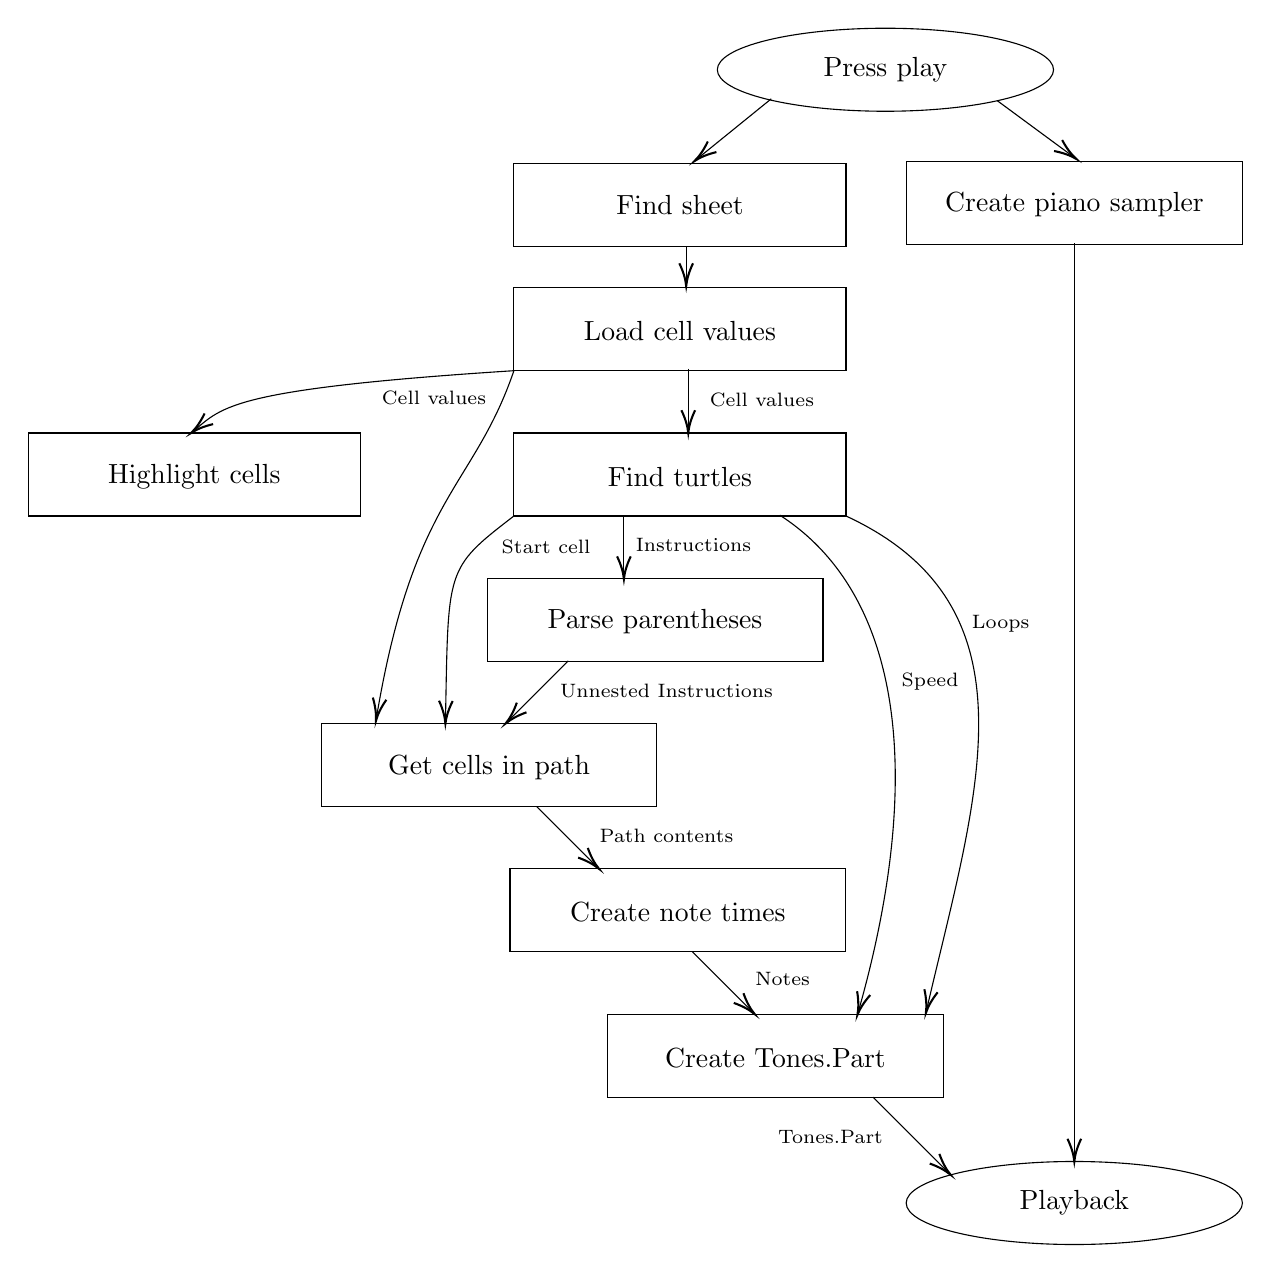
\begin{tikzpicture}[x=0.75pt,y=0.75pt,yscale=-1,xscale=1]
%uncomment if require: \path (0,604); %set diagram left start at 0, and has height of 604

%Shape: Rectangle [id:dp3390223975782729]
\draw   (244.5,71) -- (404.5,71) -- (404.5,111) -- (244.5,111) -- cycle ;

%Shape: Rectangle [id:dp7168559924493858]
\draw   (244.5,131) -- (404.5,131) -- (404.5,171) -- (244.5,171) -- cycle ;

%Shape: Rectangle [id:dp8835932361497658]
\draw   (433.7,70) -- (595.5,70) -- (595.5,110) -- (433.7,110) -- cycle ;

%Shape: Rectangle [id:dp9464422191216635]
\draw   (244.5,201) -- (404.5,201) -- (404.5,241) -- (244.5,241) -- cycle ;

%Shape: Rectangle [id:dp6384624480751633]
\draw   (231.6,271) -- (393.4,271) -- (393.4,311) -- (231.6,311) -- cycle ;

%Shape: Rectangle [id:dp2927464084046889]
\draw   (151.6,341) -- (313.4,341) -- (313.4,381) -- (151.6,381) -- cycle ;

%Shape: Rectangle [id:dp9052659554068596]
\draw   (242.6,411) -- (404.4,411) -- (404.4,451) -- (242.6,451) -- cycle ;

%Shape: Rectangle [id:dp5637329489183025]
\draw   (289.6,481) -- (451.4,481) -- (451.4,521) -- (289.6,521) -- cycle ;

%Curve Lines [id:da3917180624639185]
\draw    (244.5,241) .. controls (211.17,266.67) and (212.98,265.81) .. (211.52,339.88) ;
\draw [shift={(211.5,341)}, rotate = 271.14] [color={rgb, 255:red, 0; green, 0; blue, 0 }  ][line width=0.75]    (10.93,-3.29) .. controls (6.95,-1.4) and (3.31,-0.3) .. (0,0) .. controls (3.31,0.3) and (6.95,1.4) .. (10.93,3.29)   ;

%Straight Lines [id:da6961662223442007]
\draw    (297.5,241) -- (297.5,269.4) ;
\draw [shift={(297.5,271.4)}, rotate = 270] [color={rgb, 255:red, 0; green, 0; blue, 0 }  ][line width=0.75]    (10.93,-3.29) .. controls (6.95,-1.4) and (3.31,-0.3) .. (0,0) .. controls (3.31,0.3) and (6.95,1.4) .. (10.93,3.29)   ;

%Curve Lines [id:da9168950950169605]
\draw    (372.6,240.6) .. controls (431.31,278.41) and (442.88,365.52) .. (410.49,479.68) ;
\draw [shift={(410,481.4)}, rotate = 286.01] [color={rgb, 255:red, 0; green, 0; blue, 0 }  ][line width=0.75]    (10.93,-3.29) .. controls (6.95,-1.4) and (3.31,-0.3) .. (0,0) .. controls (3.31,0.3) and (6.95,1.4) .. (10.93,3.29)   ;

%Curve Lines [id:da7972588626438504]
\draw    (404.5,241) .. controls (499.03,284.78) and (467.32,375.49) .. (443.36,478.84) ;
\draw [shift={(443,480.4)}, rotate = 282.99] [color={rgb, 255:red, 0; green, 0; blue, 0 }  ][line width=0.75]    (10.93,-3.29) .. controls (6.95,-1.4) and (3.31,-0.3) .. (0,0) .. controls (3.31,0.3) and (6.95,1.4) .. (10.93,3.29)   ;

%Straight Lines [id:da6822022155717844]
\draw    (270.7,310.8) -- (241.91,339.59) ;
\draw [shift={(240.5,341)}, rotate = 315] [color={rgb, 255:red, 0; green, 0; blue, 0 }  ][line width=0.75]    (10.93,-3.29) .. controls (6.95,-1.4) and (3.31,-0.3) .. (0,0) .. controls (3.31,0.3) and (6.95,1.4) .. (10.93,3.29)   ;

%Straight Lines [id:da4884596231580207]
\draw    (255.5,381) -- (284.09,409.59) ;
\draw [shift={(285.5,411)}, rotate = 225] [color={rgb, 255:red, 0; green, 0; blue, 0 }  ][line width=0.75]    (10.93,-3.29) .. controls (6.95,-1.4) and (3.31,-0.3) .. (0,0) .. controls (3.31,0.3) and (6.95,1.4) .. (10.93,3.29)   ;

%Straight Lines [id:da9233366942734922]
\draw    (330.5,451) -- (359.09,479.59) ;
\draw [shift={(360.5,481)}, rotate = 225] [color={rgb, 255:red, 0; green, 0; blue, 0 }  ][line width=0.75]    (10.93,-3.29) .. controls (6.95,-1.4) and (3.31,-0.3) .. (0,0) .. controls (3.31,0.3) and (6.95,1.4) .. (10.93,3.29)   ;

%Straight Lines [id:da3670498457872964]
\draw    (417.5,521) -- (453.49,556.99) ;
\draw [shift={(454.9,558.4)}, rotate = 225] [color={rgb, 255:red, 0; green, 0; blue, 0 }  ][line width=0.75]    (10.93,-3.29) .. controls (6.95,-1.4) and (3.31,-0.3) .. (0,0) .. controls (3.31,0.3) and (6.95,1.4) .. (10.93,3.29)   ;

%Straight Lines [id:da28794703530347365]
\draw    (327.5,111) -- (327.5,128.2) ;
\draw [shift={(327.5,130.2)}, rotate = 270] [color={rgb, 255:red, 0; green, 0; blue, 0 }  ][line width=0.75]    (10.93,-3.29) .. controls (6.95,-1.4) and (3.31,-0.3) .. (0,0) .. controls (3.31,0.3) and (6.95,1.4) .. (10.93,3.29)   ;

%Straight Lines [id:da33376731250782754]
\draw    (328.5,170) -- (328.5,199) ;
\draw [shift={(328.5,201)}, rotate = 270] [color={rgb, 255:red, 0; green, 0; blue, 0 }  ][line width=0.75]    (10.93,-3.29) .. controls (6.95,-1.4) and (3.31,-0.3) .. (0,0) .. controls (3.31,0.3) and (6.95,1.4) .. (10.93,3.29)   ;

%Curve Lines [id:da2676626927985757]
\draw    (244.5,171) .. controls (225.1,227.72) and (196.29,230.77) .. (178.27,338.17) ;
\draw [shift={(178,339.8)}, rotate = 279.38] [color={rgb, 255:red, 0; green, 0; blue, 0 }  ][line width=0.75]    (10.93,-3.29) .. controls (6.95,-1.4) and (3.31,-0.3) .. (0,0) .. controls (3.31,0.3) and (6.95,1.4) .. (10.93,3.29)   ;

%Straight Lines [id:da024649031996502035]
\draw    (514.5,109.6) -- (514.5,550) ;
\draw [shift={(514.5,552)}, rotate = 270] [color={rgb, 255:red, 0; green, 0; blue, 0 }  ][line width=0.75]    (10.93,-3.29) .. controls (6.95,-1.4) and (3.31,-0.3) .. (0,0) .. controls (3.31,0.3) and (6.95,1.4) .. (10.93,3.29)   ;

%Shape: Ellipse [id:dp13505581605963868]
\draw   (433.5,572) .. controls (433.5,560.95) and (469.76,552) .. (514.5,552) .. controls (559.24,552) and (595.5,560.95) .. (595.5,572) .. controls (595.5,583.05) and (559.24,592) .. (514.5,592) .. controls (469.76,592) and (433.5,583.05) .. (433.5,572) -- cycle ;

%Shape: Ellipse [id:dp006287630832967794]
\draw   (342.5,26) .. controls (342.5,14.95) and (378.76,6) .. (423.5,6) .. controls (468.24,6) and (504.5,14.95) .. (504.5,26) .. controls (504.5,37.05) and (468.24,46) .. (423.5,46) .. controls (378.76,46) and (342.5,37.05) .. (342.5,26) -- cycle ;

%Straight Lines [id:da09048722077694915]
\draw    (368.5,40) -- (333.05,68.74) ;
\draw [shift={(331.5,70)}, rotate = 320.96000000000004] [color={rgb, 255:red, 0; green, 0; blue, 0 }  ][line width=0.75]    (10.93,-3.29) .. controls (6.95,-1.4) and (3.31,-0.3) .. (0,0) .. controls (3.31,0.3) and (6.95,1.4) .. (10.93,3.29)   ;

%Straight Lines [id:da9578993167654264]
\draw    (477.5,41) -- (513.89,67.81) ;
\draw [shift={(515.5,69)}, rotate = 216.38] [color={rgb, 255:red, 0; green, 0; blue, 0 }  ][line width=0.75]    (10.93,-3.29) .. controls (6.95,-1.4) and (3.31,-0.3) .. (0,0) .. controls (3.31,0.3) and (6.95,1.4) .. (10.93,3.29)   ;

%Shape: Rectangle [id:dp25073410390478523]
\draw   (10.5,201) -- (170.5,201) -- (170.5,241) -- (10.5,241) -- cycle ;

%Curve Lines [id:da2454539812308738]
\draw    (244.5,171) .. controls (108.92,179.69) and (104.17,188.37) .. (90.53,199.75) ;
\draw [shift={(89,201)}, rotate = 321.34000000000003] [color={rgb, 255:red, 0; green, 0; blue, 0 }  ][line width=0.75]    (10.93,-3.29) .. controls (6.95,-1.4) and (3.31,-0.3) .. (0,0) .. controls (3.31,0.3) and (6.95,1.4) .. (10.93,3.29)   ;


% Text Node
\draw (324.5,91) node  [align=left] {Find sheet};
% Text Node
\draw (324.5,152) node  [align=left] {Load cell values};
% Text Node
\draw (514.6,91) node  [align=left] {Create piano sampler};
% Text Node
\draw (324.5,222) node  [align=left] {Find turtles};
% Text Node
\draw (312.5,292) node  [align=left] {Parse parentheses};
% Text Node
\draw (232.5,362) node  [align=left] {Get cells in path};
% Text Node
\draw (323.5,432) node  [align=left] {Create note times};
% Text Node
\draw (370.5,502) node  [align=left] {Create Tones.Part};
% Text Node
\draw (514.5,572) node [] [align=left] {\textcolor[rgb]{0,0,0}{Playback}};
% Text Node
\draw (260,256) node  [align=left] {{\scriptsize Start cell}};
% Text Node
\draw (331,255) node  [align=left] {{\scriptsize Instructions}};
% Text Node
\draw (445,321) node  [align=left] {{\scriptsize Speed}};
% Text Node
\draw (479,293) node  [align=left] {{\scriptsize Loops}};
% Text Node
\draw (318,325) node  [align=left] {{\scriptsize Unnested Instructions}};
% Text Node
\draw (318,395) node  [align=left] {{\scriptsize Path contents}};
% Text Node
\draw (374,464) node  [align=left] {{\scriptsize Notes}};
% Text Node
\draw (397,540) node  [align=left] {{\scriptsize Tones.Part}};
% Text Node
\draw (206,184) node  [align=left] {{\scriptsize Cell values}};
% Text Node
\draw (423.5,26) node [] [align=left] {Press play};
% Text Node
\draw (364,185) node  [align=left] {{\scriptsize Cell values}};
% Text Node
\draw (90.5,222) node  [align=left] {Highlight cells};


\end{tikzpicture}

\end{center}

\begin{algorithm}[!htbp]
\caption{Parsing bracketed expression}\label{alg:parenthesis}
\begin{algorithmic}[1]
\Procedure{parseBrackets}{$str$}

   \State $idPadding\gets \texttt{\upquote{\_\_\_}}$
   \State $unnestedStr\gets []$
   \State $deepestLevelBracketsRE\gets \texttt{RegExp(\upquote{\textbackslash\textbackslash([\^{}\textbackslash\textbackslash(\textbackslash\textbackslash)]*\textbackslash\textbackslash)})}$
   \State $replacementIDRE\gets \texttt{RegExp(\upquote{\textbackslash\textbackslash} + }idPadding\texttt{ + \upquote{([0-9]+)} + }idPadding\texttt{)}$\\

   \Procedure{replaceDeepestBracket}{$x$}
     \State \texttt{unnestedStr.push(x.substring(1, x.length-1))}
     \State \texttt{\textbf{return} idPadding + (unnestedStr.length - 1) + idPadding}
   \EndProcedure \\

   \While{\texttt{deepestLevelBracketsRE.test(str)}}
     \State \texttt{str = str.replace(deepestLevelBracketsRE,replaceDeepestBracket)}
   \EndWhile

   \State \texttt{unnestedStr[0] = str}\\

   \Procedure{reNest}{$outerStr$}
     \State $renestingStr\gets []$
     \While{There is a match of $replacementIDRE$ in $outerStr$}
       \State $matchIndex\gets$ index of the match in $outerStr$
       \State $matchID\gets$ ID of the match (number between padding)
       \State $matchString\gets$ matched string\\

       \If{$matchIndex >$ 0}
				\State $renestingStr$.push($outestStr$.substring(0, $matchIndex$))
			\EndIf
			\State $renestingStr$.push(reNest($unnestedStr$[$firstMatchID$]))
			\State $outestStr$ = $outestStr$.substring($matchIndex$ + $matchString$.length)
     \EndWhile
     \State $renestingStr$.push($outestStr$)
     \State \textbf{return} $renestingStr$
   \EndProcedure \\

   \State \textbf{return} reNest($unnestedStr$[0])

\EndProcedure
\end{algorithmic}
\end{algorithm}

\section{Simple diagrams}

Simple diagrams can be written directly in \LaTeX.  For example, see
figure~\ref{latexpic1} on page~\pageref{latexpic1} and see
figure~\ref{latexpic2} on page~\pageref{latexpic2}.

\begin{figure}
\setlength{\unitlength}{1mm}
\begin{center}
\begin{picture}(125,100)
\put(0,80){\framebox(50,10){AAA}}
\put(0,60){\framebox(50,10){BBB}}
\put(0,40){\framebox(50,10){CCC}}
\put(0,20){\framebox(50,10){DDD}}
\put(0,00){\framebox(50,10){EEE}}

\put(75,80){\framebox(50,10){XXX}}
\put(75,60){\framebox(50,10){YYY}}
\put(75,40){\framebox(50,10){ZZZ}}

\put(25,80){\vector(0,-1){10}}
\put(25,60){\vector(0,-1){10}}
\put(25,50){\vector(0,1){10}}
\put(25,40){\vector(0,-1){10}}
\put(25,20){\vector(0,-1){10}}

\put(100,80){\vector(0,-1){10}}
\put(100,70){\vector(0,1){10}}
\put(100,60){\vector(0,-1){10}}
\put(100,50){\vector(0,1){10}}

\put(50,65){\vector(1,0){25}}
\put(75,65){\vector(-1,0){25}}
\end{picture}
\end{center}
\caption{A picture composed of boxes and vectors.}
\label{latexpic1}
\end{figure}

\begin{figure}
\setlength{\unitlength}{1mm}
\begin{center}

\begin{picture}(100,70)
\put(47,65){\circle{10}}
\put(45,64){abc}

\put(37,45){\circle{10}}
\put(37,51){\line(1,1){7}}
\put(35,44){def}

\put(57,25){\circle{10}}
\put(57,31){\line(-1,3){9}}
\put(57,31){\line(-3,2){15}}
\put(55,24){ghi}

\put(32,0){\framebox(10,10){A}}
\put(52,0){\framebox(10,10){B}}
\put(37,12){\line(0,1){26}}
\put(37,12){\line(2,1){15}}
\put(57,12){\line(0,2){6}}
\end{picture}

\end{center}
\caption{A diagram composed of circles, lines and boxes.}
\label{latexpic2}
\end{figure}



\section{Adding more complicated graphics}

The use of \LaTeX\ format can be tedious and it is often better to use
encapsulated postscript (EPS) or PDF to represent complicated graphics.
Figure~\ref{epsfig} and~\ref{xfig} on page \pageref{xfig} are
examples. The second figure was drawn using \texttt{xfig} and exported in
{\tt.eps} format. This is my recommended way of drawing all diagrams.


\begin{figure}[tbh]
\centerline{\includegraphics{figs/cuarms.pdf}}
\caption{Example figure using encapsulated postscript}
\label{epsfig}
\end{figure}

\begin{figure}[tbh]
\vspace{4in}
\caption{Example figure where a picture can be pasted in}
\label{pastedfig}
\end{figure}


\begin{figure}[tbh]
\centerline{\includegraphics{figs/diagram.pdf}}
\caption{Example diagram drawn using \texttt{xfig}}
\label{xfig}
\end{figure}


\chapter{Implementation}

In this chapter I shall first explain how the turtles, using the movement instructions defined previously, are defined and controlled. The remaining features in the initial prototype will be explained. The format and results of the formative evaluation using this initial prototype shall be summarised. I shall then cover the design decisions and changes that were made to the Excello prototype during the participatory design process. Then, how Excello has been implemented will be described followed by the MIDI to Excello converter. The chapter concludes with an overview of the project repository.

\section{Initial Prototype}

Notes and turtles can be defined in any cell in the spreadsheet. When the Excello add-in is opened, a window will open in the right side of Excel. This contains a play and stop button which can be used to launch all the turtles defined in the spreadsheet and initiate playback. Playback is a realistic piano sound.

A summary of the musical elements that can be put in cells and that will be interpreted by turtles is shown in table \ref{tab:cells}

\begin{table}
\centering
% \caption{Grammar Rules for the turtle movement instructions. $z \in \Z$}
\caption{Definition of notes in cells.}
\begin{tabular}{|l|l|} \hline
\textbf{Interpretation}&\textbf{Format}\\ \hline
Note& Note name (A-G), optional accidentals and octave \\
&number e.g. \texttt{F\#4}\\ \hline
Sustain& \texttt{s}\\ \hline
Multiple notes& Notes, rests or sustains separated by a comma. Rests \\
subdivided in time& must be a space or an empty string e.g. \texttt{E4,,C4,s}\\ \hline
Rest& Any cell not interpreted as a note, sustain or multi-note. \\ \hline
\end{tabular}
\label{tab:cells}
\end{table}

\subsection{Turtles}

Notes are played by defining and launching turtles to navigate the spreadsheet. Turtles are defined as follows:

\texttt{!turtle(<Starting Cell>, <Movement>, <Speed>, <Number of Loops>)}

\subsubsection{Activation}

The "\texttt{!}" dictates that the turtle will be activated when the play button in the add-in window is pressed. Just like many digital audio workstations allow muting and soloing of tracks, this can be used to quickly modify which turtles will play without losing the definition of the turtle.

\subsubsection{Starting Cell}

The starting cell of the turtle is given by the cell reference. As with conventional Excel formulae, columns are defined in base 26 using the letters of the alphabet and rows are numbered using the integers. A cell is defined by the concatenation of the column letters and row number. This cell will be played and is the first cell in the path of the turtle.

As each turtle only plays one note at a time, multiple turtles must be defined to play polyphonic music such as chords. It was believed that in these cases the turtles may follow identical paths but in adjacent rows or columns. Multiple turtles following identical paths but starting from adjacent cells can be defined using the existing Excel range notation to define the starting cells. "\texttt{A2:A5}" would define four turtles in the cells A2,A3,A4,A5. This prevents the writing of multiple turtle definitions differing in only the start cell row.

\subsubsection{Movement}

The turtles start facing north. The design of the language used to define turtle movement has been discussed in the preparation chapter. Using brackets to repeat multiple instructions within the turtle's instructions was not implemented by the start of the participatory design process.

\subsubsection{Speed}

An optional third argument can be provided to defined the speed at which the turtle moves through the grid. If the argument is not provided, the turtle moves at 160 cells per minute through the grid. The speed argument defines the speed relative to 160 cells per minute. Therefore if the argument "\texttt{2}" was provided, this would move through the grid at 320 cells per minute. This relative system was used so it would be easier to tell the speed relation between two turtles. This would be particularly beneficial for phase music. Arbitrary maths can be provided for this argument and it will be evaluated. This can be used to define a turtle  speed is an irrational multiple of another's.

\subsubsection{Number of Loops}

An optional fourth argument defines the number of times the path of the turtle is played. If committed the turtle will loop infinitely. This was included so that repeating parts (e.g. the cello part of Pachabel's Canon in D) need only defining once but can be played repetitively.

\subsection{Highlighting}

In order to assist in the recognition of notes and turtles, when the play button is pressed, cells are highlighted depending on their contents. Cells containing activated or deactivated definitions of turtles are highlighted green. Cells containing definitions of notes, or multiple notes, are highlighted red, with cells only containing a sustain highlighted a lighter red, to show a correspondance to notes whilst not carrying quite so much information.

\subsection{Chord input}

In order to maintain musical abstractions of chords and arpeggios \footnote{Where the notes of a chord are played in rising or descending order} whilst keeping to paradigm of a turtle being responsible for up to one note at any time, a tool to add chords and arpeggios is available. The note, type (over 100 available), inversion and starting octave of the chord are inputted in four drop-down selectors and the notes making up that chord are entered into the grid using the insert button. If a single cell or range taller than it is wide is highlighted in the spreadsheet, the notes will be inserted in adjacent vertical cells starting at the top-left of the range. Otherwise, the notes will be inserted horizontally. This means whether the turtles are moving horizontally or vertically both chords and arpeggios can be easily defined. As a result, helpful musical abstractions are still available whilst keeping the cleanness of the turtle system.

\section{Formative Evaluation}

In order to guide the development of the project to best suite the users, participants were involved in formative evaluation. 21 participants took place in the participatory design process. Participants were all University of Cambridge students, across a range of subjects, but all musical. Initially, individual meetings were held with each participant. A tutorial of the initial prototype was given followed by the carrying out of a short exercise lasting 15-20 minutes in most cases. After both the tutorial and the exercise, users were asked to comment on how they found Excello. Particular attention was drawn to actions that they found particularly unintuitive or required notable mental effort. Comparisons were also made to the musical interfaces that participants were already familiar with. The sessions were audio recorded in order to prevent the jotting down of notes causing delays, and later notes were made from these recordings. The ethical and data handling procedures that were carried out shall be discussed in the evaluation chapter.

In order to simulate the most likely ways in which Excello would be used, participants were given the freedom to carry out an exercise of their choice. In many cases this was transcribing an exiting piece from memory or from traditional western notation into the Excello notation. Two tasks were provided to choose from if participants had no immediate inspiration. These were to transcribe a piece of music from western notation or to make changes to an existing piece in the Excello notation.

These sessions were carried out at the beginning of Lent term 2019. Participants were asked if they would be willing to continue using Excello personally from their initial session until the summative evaluation sessions, eight weeks later. This gave time for additional feedback to be given as participants used Excello in their own time. It also ensured that the summative evaluation carried out would be done so by users with sufficient experience of the interface. Participants were encouraged to get in contact with any additional issues or suggestions they had during this time.

\subsection{Issues and Suggestions}

The issues and suggestions that arose during the participatory design period have been categorised and summarised below.

\subsubsection{Turtle Notation}

Having dynamic instructions within the turtle was found to make it harder to extract the path that the turtle followed as not all instructions related to the way in which the turtle moves. As the dynamics weren't next to the notes they corresponded to, it was challenging to establish which volume a given note would be played at or where to place the dynamic instructions within the turtle to correspond to a certain note positioned elsewhere in the spreadsheet. In the initial prototype there was no way to assign a dynamic to the first note without having the starting cell being empty. The addition of this empty cell could be inconvenient for looping parts as this empty cell would be included in the loop. Users who were not familiar with the dynamic markings of western notation found them unintuitive. Furthermore, it was noted that these discrete markings do not make available the continuous volume scale that could be possible with the interface.

When trying to transcribe a piece in an exact tempo, having to divide the speed by 160 in order to enter a relative speed caused unnecessary work. There was forgetfulness as to the whether relative speed referred to how long or how quickly the turtle moved.

Having completed the tutorial, users often has to check which arguments appeared where within the turtle definition or what the arguments were.

When parsing the instruction, as the number of dynamics and movement instructions grew and the instruction became long, it could become quite tough to establish how the turtle would behave. As "\texttt{s}" could be used to indicate sustain within cells, some users confused the "\texttt{s}" within the turtle instructions to mean sustain and not south.

\subsubsection{Feedback}

Having clicked the play button it was often not clear if this had been registered. Especially if the Excel workbook was saving, and this caused a delay in Excello being able to access the spreadsheet. It was also requested if it would be possible to see a summary of where the active turtle were in addition to them being highlighted green. If a turtle had accidentally been left activated, the entire grid had to be searched in order to locate it.

\subsubsection{MIDI conversions}

Many users, especially those who used production software such as GarageBand and Logic, said that it would be helpful to be able to interact with MIDI files. Being able to use Excello to create their chord sequences and bass lines before adding additional effects and recorded lines in their digital audio work stations would require a MIDI export. In addition, if working with an existing MIDI file, it would be convenient to be able to convert that into the Excello notation.

\subsubsection{Sources of effort when writing}

Once notes had been inputted into the grid, often in a single straight line, the number of cells had to be counted so the turtle could be moved the correct number of cells. Whilst Excel allows users to highlight a selection of cells and have an immediate output of how many cells are highlighted without any formula being written, this is still an unproductive use of time. Some users would simply instruct the turtle to move forward significantly more steps than required to prevent this counting, but this is not feasible for looping parts. It was suggested that turtles could figure out how far they should move so that the instruction didn't need editing when more notes were added. This was particularly inconvenient when users were writing out a piece and periodically testing what they had written so far.

If instructions involved repeats such as repeatedly moving to the end of a line and jumping down a few cells and back to the beginning of the line, instructions within the turtles required a lot of repetition.

If writing out a melodic line consisting of small movements, many of the notes would take place in the same octave. As such, it was tiresome to have to repeatedly write out the octave number when this was barely changing. One user made a comparison to LilyPond \footnote{A program for music notation using text notation.} \cite{sandberg:lily} where if the length of a note is not defined, the last defined note length would be used.

Some users said they would find it more intuitive to think of a melodic line in terms of the intervals between notes as opposed to the name of each note. If a piece contained a melodic line that was modulated \footnote{Where every note has been moved up or down in pitch by the same amount.}, the modulated part had to be written out again and could not be derived quicker from the original version.

\subsubsection{Chords}

Whilst the variety of available chord types was appreciated, most users used a very small subset of these but still had to scroll through the whole list to find these. Separating the more common chords for easier access was requested. In the initial prototype, the notes were inserted from low to high. This meant that notes inserted in a vertical line had the lowest note at the top with notes increasing in pitch proceeding down the column. In western staff notation, higher pitch notes appear higher up the staff. As a result, it was suggested that inverting the order would be more intuitive. In the initial interface it was also unclear what the different drop downs corresponded to, with some users selecting the "7" from the octave number in order to try and insert a Maj7 chord.

\subsubsection{Activation of turtles}

When toggling the activation of a turtle, it was very tedious to have to enter the edit mode for each cell containing a turtle definition and add or remove the exclamation mark. This was particularly so if a piece had multiple turtle definitions.

\section{Second Prototype}

Following the formative evaluation sessions carried out with the participants and the feedback that was received, a series of additions and modifications were made to the prototype to solve the problems and opportunities brought up.

\subsection{Dynamics}

In order to assist users in extracting the path that the turtles follow from the instructions and pairing notes with their volume, dynamics are instead inserted in the cells along with the notes. A dynamic instruction is added after the note, separated by a space as in Manhattan \cite{nash:manhattan}. As before, this will persist for all following notes until the volume is redefined. By moving the dynamics into the cell there is a tradeoff. A single turtle definition with multiple start cells can now play parts of different volume. However, notes in the grid are limited to only being played at the given volume. To play the same notes at a different volume would require a different path to be followed by the turtle where the cells defining the volume are missed and other cells are played. Overall, the new system was believed to be more preferable.

In order to be able to make use of a full continuous dynamic scale, in addition to the existing dynamic symbols available, a number between 0 and 1 can be provided where 0 will be silent and 1 is equivalent to fff.

\subsection{Nested Instructions}

The initial language design included the use of nested instruction in order to allow for easy repetition of turtle movements. This was not implemented when the first formative evaluation sessions took place. However, this should help reduce the length of turtle instructions and allow for repeated sections or movements to be more easily incorporated. A series of instructions placed within parentheses with a number immediately following the closing parenthesis will be repeated that number of times. Whilst the fourth argument of the turtle will simply repeat the musical output of the turtle, repetitions within the turtle instruction allow paths to be defined more concisely.

\subsection{Absolute Tempo}

The speed at which the turtle moves is now defined by cells per minute, rather than the relative value used initially. However, values less than 10 were interpreted in the original relative way to maintain backwards compatibility for the participant's existing work. To maintain consistency in a production version, this would be removed so speed must be defined absolutely. This also ensures that the values given for speed and dynamics will be of different orders of magnitude and hence reduce the confusion that can occur between them.

\subsection{Custom Excel Functions}

Two custom Excel functions were implemented to aid in the composition of music within Excel. One to aid with inserting turtles into the grid and a second to transpose notes.

\subsubsection{Excello.Turtle}

Many users had commented they forgot which arguments go where within the turtle. By adding custom Excel functions the existing formulae writing tools provided within Excel can be utilised. When using a built in formula, a prompt appears informing users which arguments go where and whether they are optional. The output of this function is text used to define a turtle if written manually. This also allows other cells to be referenced for the arguments of the turtle function. For example a cell could have speed defined that all other turtles reference. As a result, the speed of all turtles could be modified by changing this single value. This also allows relative tempos to be easily implemented again as the speed argument of the turtle could be defined as a relative speed mutliplied by the global speed (given as a cell referece).

\subsubsection{Excello.Modulate}

The implementation of a function to modulate notes both allows for the easy modulation of existing sections of a piece and also the definition of a melodic line by the intervals between the notes. The function takes the contents of a cell where a note is defined and an interval and outputs the note transposed by that interval. A section can be modulated by calling this function on the first note with a provided interval and using the existing drag-fill functionality of Excel to modulate all notes. By using the previous note that has just been transposed and one of a series of intervals as the arguments, a melodic line can quickly be produced from a starting note and a series of intervals.

%  \ref{examples}

\subsection{Sustain}

In order to prevent confusion between the instruction for a turtle to face south and for a note to be sustained. The symbol "\texttt{-}" has been chosen to sustain a note. This was chosen because it is light and also has some similarity to a tie \footnote{A line to increase the length of a note by joining to another.}. The use of an "\texttt{s}" is still interpreted as a sustain to maintain backwards compatibility for the existing work of the participants.

\subsection{Active Turtles}

In order to provide feedback that turtle definitions have been recognised, in addition to green highlighting, a list of the active turtles is given below the play button. This also assists in finding any spurious turtles that were not intended to be activated.

\subsection{Automatic Movement}

To prevent the number of cells in a line needing counting, a turtle can be instructed to move as far as there are notes defined in the direction it is currently facing. This means that if more notes are added on this line, the turtle instructions do not need editing before pressing play. There may be cases where a part is meant to finish with a number of rests. As a rest is notated with a blank cell, a method of increasing the length of the path to include these rests is required. A rest can be given explicitly with a "\texttt{.}" allowing the distance distance travelled by the turtle when moving automatically to be increased. This would be required if multiple turtles were defining a repeating section where one does not have the final cell of the section being a note, sustain or multi-note cell. Without an explicit rest the turtle would stop and repeat too soon and the parts would be out of phase.

\subsection{Inferred Octave}

To prevent the octave number needing writing every time a note in defined, the octave number can be inferred by the program if it is omitted. There were two methods under consideration. Firstly, given that most intervals within music are small, the nearest note could be inferred. This means that a scale would only need the octave defining in the first note. Whilst this method would likely require the least explicit statement of octave number it would be non-trivial to figure out the octave a given note is played in. The last defined octave in the path would need finding and then the subsequent notes would have to be walked through keeping track of which octave is being played. The second consideration was to always use the last defined octave. Whilst this may require reasonable octave definition around the boundary between octaves, it is easier to find what octave a note is played at as it is simply the last defined octave in the path.

\subsection{Chords}

In order to assist in the entering of common chords, common chord types are repeated in a separate group  at the top of the type selection drop-down. The layout of the chord drop-downs was improved with labels added to make it clearer what the different values would refer to. If the notes were entered vertically, the order was reversed to have a greater correspondence with traditional staff notation.

\subsection{Activation of turtles}

A "Toggle Activation" button was added to the add-in window. When a cell or range is highlighted in the spreadsheet, the activation of any turtle definitions in this range will be toggled when the button is pressed.  This significantly increases the ease with which turtles can be deselected as only two clicks are required as opposed to having to enter the cell edit mode and add or remove an exclamation mark.

\section{How it works}

\section{MIDI Converter}

\section{Repository Overview}

% \section{Verbatim text}
%
% Verbatim text can be included using \verb|\begin{verbatim}| and
% \verb|\end{verbatim}|. I normally use a slightly smaller font and
% often squeeze the lines a little closer together, as in:
%
% {\renewcommand{\baselinestretch}{0.8}\small
% \begin{verbatim}
%   export function parseBrackets(str: string) {
%
%   	var unnestedStr = ['will become highest level'];
%   	var idPadding = '__';
%   	var deepestLevelBracketsRE = new RegExp('\\([^\\(\\)]*\\)');
%
%   	while (deepestLevelBracketsRE.test(str)) {
%   		str = str.replace(deepestLevelBracketsRE,function(x) {
%   			unnestedStr.push(x.substring(1, x.length-1));
%   			return idPadding + (unnestedStr.length - 1) + idPadding;
%   		});
%   	}
%   	unnestedStr[0] = str;
%
%   	var replacementIDRE = new RegExp('\\' + idPadding + '([0-9]+)' + idPadding);
%
%   	// transform references to tree
%   	function reNest (outestStr: string) {
%   		var renestingStr = [];
%   		var match;
%
%   		while (match = replacementIDRE.exec(outestStr)) {
%
%   			var matchIndex = match.index;
%   			var firstMatchID = match[1];
%   			var fullStringMatched = match[0];
%
%   			// push what was before
%   			if (matchIndex > 0) {
%   				renestingStr.push(outestStr.substring(0, matchIndex))
%   			}
%   			//perform recursively
%   			renestingStr.push(reNest(unnestedStr[firstMatchID]))
%   			// remove the string that has been processed
%   			outestStr = outestStr.substring(matchIndex + fullStringMatched.length)
%   		}
%   		renestingStr.push(outestStr)
%   		return renestingStr
%   	}
%
%   	return reNest(unnestedStr[0])
%   }
% \end{verbatim}
% }

\begin{center}


\tikzset{every picture/.style={line width=0.75pt}} %set default line width to 0.75pt

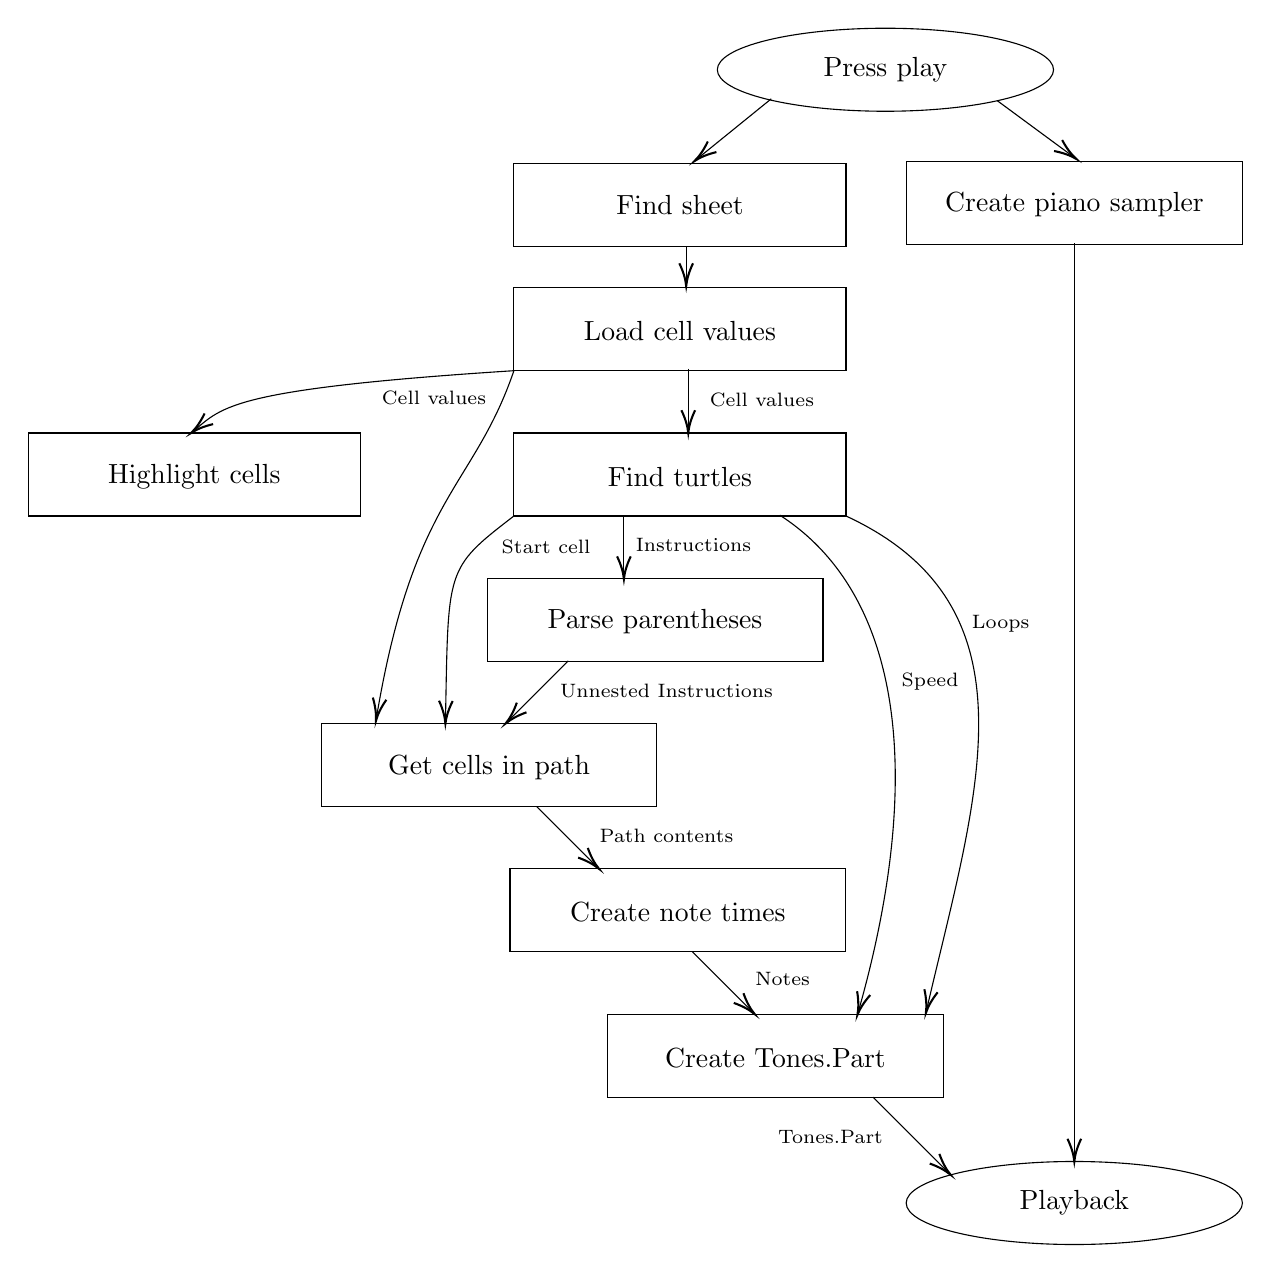
\begin{tikzpicture}[x=0.75pt,y=0.75pt,yscale=-1,xscale=1]
%uncomment if require: \path (0,604); %set diagram left start at 0, and has height of 604

%Shape: Rectangle [id:dp3390223975782729]
\draw   (244.5,71) -- (404.5,71) -- (404.5,111) -- (244.5,111) -- cycle ;

%Shape: Rectangle [id:dp7168559924493858]
\draw   (244.5,131) -- (404.5,131) -- (404.5,171) -- (244.5,171) -- cycle ;

%Shape: Rectangle [id:dp8835932361497658]
\draw   (433.7,70) -- (595.5,70) -- (595.5,110) -- (433.7,110) -- cycle ;

%Shape: Rectangle [id:dp9464422191216635]
\draw   (244.5,201) -- (404.5,201) -- (404.5,241) -- (244.5,241) -- cycle ;

%Shape: Rectangle [id:dp6384624480751633]
\draw   (231.6,271) -- (393.4,271) -- (393.4,311) -- (231.6,311) -- cycle ;

%Shape: Rectangle [id:dp2927464084046889]
\draw   (151.6,341) -- (313.4,341) -- (313.4,381) -- (151.6,381) -- cycle ;

%Shape: Rectangle [id:dp9052659554068596]
\draw   (242.6,411) -- (404.4,411) -- (404.4,451) -- (242.6,451) -- cycle ;

%Shape: Rectangle [id:dp5637329489183025]
\draw   (289.6,481) -- (451.4,481) -- (451.4,521) -- (289.6,521) -- cycle ;

%Curve Lines [id:da3917180624639185]
\draw    (244.5,241) .. controls (211.17,266.67) and (212.98,265.81) .. (211.52,339.88) ;
\draw [shift={(211.5,341)}, rotate = 271.14] [color={rgb, 255:red, 0; green, 0; blue, 0 }  ][line width=0.75]    (10.93,-3.29) .. controls (6.95,-1.4) and (3.31,-0.3) .. (0,0) .. controls (3.31,0.3) and (6.95,1.4) .. (10.93,3.29)   ;

%Straight Lines [id:da6961662223442007]
\draw    (297.5,241) -- (297.5,269.4) ;
\draw [shift={(297.5,271.4)}, rotate = 270] [color={rgb, 255:red, 0; green, 0; blue, 0 }  ][line width=0.75]    (10.93,-3.29) .. controls (6.95,-1.4) and (3.31,-0.3) .. (0,0) .. controls (3.31,0.3) and (6.95,1.4) .. (10.93,3.29)   ;

%Curve Lines [id:da9168950950169605]
\draw    (372.6,240.6) .. controls (431.31,278.41) and (442.88,365.52) .. (410.49,479.68) ;
\draw [shift={(410,481.4)}, rotate = 286.01] [color={rgb, 255:red, 0; green, 0; blue, 0 }  ][line width=0.75]    (10.93,-3.29) .. controls (6.95,-1.4) and (3.31,-0.3) .. (0,0) .. controls (3.31,0.3) and (6.95,1.4) .. (10.93,3.29)   ;

%Curve Lines [id:da7972588626438504]
\draw    (404.5,241) .. controls (499.03,284.78) and (467.32,375.49) .. (443.36,478.84) ;
\draw [shift={(443,480.4)}, rotate = 282.99] [color={rgb, 255:red, 0; green, 0; blue, 0 }  ][line width=0.75]    (10.93,-3.29) .. controls (6.95,-1.4) and (3.31,-0.3) .. (0,0) .. controls (3.31,0.3) and (6.95,1.4) .. (10.93,3.29)   ;

%Straight Lines [id:da6822022155717844]
\draw    (270.7,310.8) -- (241.91,339.59) ;
\draw [shift={(240.5,341)}, rotate = 315] [color={rgb, 255:red, 0; green, 0; blue, 0 }  ][line width=0.75]    (10.93,-3.29) .. controls (6.95,-1.4) and (3.31,-0.3) .. (0,0) .. controls (3.31,0.3) and (6.95,1.4) .. (10.93,3.29)   ;

%Straight Lines [id:da4884596231580207]
\draw    (255.5,381) -- (284.09,409.59) ;
\draw [shift={(285.5,411)}, rotate = 225] [color={rgb, 255:red, 0; green, 0; blue, 0 }  ][line width=0.75]    (10.93,-3.29) .. controls (6.95,-1.4) and (3.31,-0.3) .. (0,0) .. controls (3.31,0.3) and (6.95,1.4) .. (10.93,3.29)   ;

%Straight Lines [id:da9233366942734922]
\draw    (330.5,451) -- (359.09,479.59) ;
\draw [shift={(360.5,481)}, rotate = 225] [color={rgb, 255:red, 0; green, 0; blue, 0 }  ][line width=0.75]    (10.93,-3.29) .. controls (6.95,-1.4) and (3.31,-0.3) .. (0,0) .. controls (3.31,0.3) and (6.95,1.4) .. (10.93,3.29)   ;

%Straight Lines [id:da3670498457872964]
\draw    (417.5,521) -- (453.49,556.99) ;
\draw [shift={(454.9,558.4)}, rotate = 225] [color={rgb, 255:red, 0; green, 0; blue, 0 }  ][line width=0.75]    (10.93,-3.29) .. controls (6.95,-1.4) and (3.31,-0.3) .. (0,0) .. controls (3.31,0.3) and (6.95,1.4) .. (10.93,3.29)   ;

%Straight Lines [id:da28794703530347365]
\draw    (327.5,111) -- (327.5,128.2) ;
\draw [shift={(327.5,130.2)}, rotate = 270] [color={rgb, 255:red, 0; green, 0; blue, 0 }  ][line width=0.75]    (10.93,-3.29) .. controls (6.95,-1.4) and (3.31,-0.3) .. (0,0) .. controls (3.31,0.3) and (6.95,1.4) .. (10.93,3.29)   ;

%Straight Lines [id:da33376731250782754]
\draw    (328.5,170) -- (328.5,199) ;
\draw [shift={(328.5,201)}, rotate = 270] [color={rgb, 255:red, 0; green, 0; blue, 0 }  ][line width=0.75]    (10.93,-3.29) .. controls (6.95,-1.4) and (3.31,-0.3) .. (0,0) .. controls (3.31,0.3) and (6.95,1.4) .. (10.93,3.29)   ;

%Curve Lines [id:da2676626927985757]
\draw    (244.5,171) .. controls (225.1,227.72) and (196.29,230.77) .. (178.27,338.17) ;
\draw [shift={(178,339.8)}, rotate = 279.38] [color={rgb, 255:red, 0; green, 0; blue, 0 }  ][line width=0.75]    (10.93,-3.29) .. controls (6.95,-1.4) and (3.31,-0.3) .. (0,0) .. controls (3.31,0.3) and (6.95,1.4) .. (10.93,3.29)   ;

%Straight Lines [id:da024649031996502035]
\draw    (514.5,109.6) -- (514.5,550) ;
\draw [shift={(514.5,552)}, rotate = 270] [color={rgb, 255:red, 0; green, 0; blue, 0 }  ][line width=0.75]    (10.93,-3.29) .. controls (6.95,-1.4) and (3.31,-0.3) .. (0,0) .. controls (3.31,0.3) and (6.95,1.4) .. (10.93,3.29)   ;

%Shape: Ellipse [id:dp13505581605963868]
\draw   (433.5,572) .. controls (433.5,560.95) and (469.76,552) .. (514.5,552) .. controls (559.24,552) and (595.5,560.95) .. (595.5,572) .. controls (595.5,583.05) and (559.24,592) .. (514.5,592) .. controls (469.76,592) and (433.5,583.05) .. (433.5,572) -- cycle ;

%Shape: Ellipse [id:dp006287630832967794]
\draw   (342.5,26) .. controls (342.5,14.95) and (378.76,6) .. (423.5,6) .. controls (468.24,6) and (504.5,14.95) .. (504.5,26) .. controls (504.5,37.05) and (468.24,46) .. (423.5,46) .. controls (378.76,46) and (342.5,37.05) .. (342.5,26) -- cycle ;

%Straight Lines [id:da09048722077694915]
\draw    (368.5,40) -- (333.05,68.74) ;
\draw [shift={(331.5,70)}, rotate = 320.96000000000004] [color={rgb, 255:red, 0; green, 0; blue, 0 }  ][line width=0.75]    (10.93,-3.29) .. controls (6.95,-1.4) and (3.31,-0.3) .. (0,0) .. controls (3.31,0.3) and (6.95,1.4) .. (10.93,3.29)   ;

%Straight Lines [id:da9578993167654264]
\draw    (477.5,41) -- (513.89,67.81) ;
\draw [shift={(515.5,69)}, rotate = 216.38] [color={rgb, 255:red, 0; green, 0; blue, 0 }  ][line width=0.75]    (10.93,-3.29) .. controls (6.95,-1.4) and (3.31,-0.3) .. (0,0) .. controls (3.31,0.3) and (6.95,1.4) .. (10.93,3.29)   ;

%Shape: Rectangle [id:dp25073410390478523]
\draw   (10.5,201) -- (170.5,201) -- (170.5,241) -- (10.5,241) -- cycle ;

%Curve Lines [id:da2454539812308738]
\draw    (244.5,171) .. controls (108.92,179.69) and (104.17,188.37) .. (90.53,199.75) ;
\draw [shift={(89,201)}, rotate = 321.34000000000003] [color={rgb, 255:red, 0; green, 0; blue, 0 }  ][line width=0.75]    (10.93,-3.29) .. controls (6.95,-1.4) and (3.31,-0.3) .. (0,0) .. controls (3.31,0.3) and (6.95,1.4) .. (10.93,3.29)   ;


% Text Node
\draw (324.5,91) node  [align=left] {Find sheet};
% Text Node
\draw (324.5,152) node  [align=left] {Load cell values};
% Text Node
\draw (514.6,91) node  [align=left] {Create piano sampler};
% Text Node
\draw (324.5,222) node  [align=left] {Find turtles};
% Text Node
\draw (312.5,292) node  [align=left] {Parse parentheses};
% Text Node
\draw (232.5,362) node  [align=left] {Get cells in path};
% Text Node
\draw (323.5,432) node  [align=left] {Create note times};
% Text Node
\draw (370.5,502) node  [align=left] {Create Tones.Part};
% Text Node
\draw (514.5,572) node [] [align=left] {\textcolor[rgb]{0,0,0}{Playback}};
% Text Node
\draw (260,256) node  [align=left] {{\scriptsize Start cell}};
% Text Node
\draw (331,255) node  [align=left] {{\scriptsize Instructions}};
% Text Node
\draw (445,321) node  [align=left] {{\scriptsize Speed}};
% Text Node
\draw (479,293) node  [align=left] {{\scriptsize Loops}};
% Text Node
\draw (318,325) node  [align=left] {{\scriptsize Unnested Instructions}};
% Text Node
\draw (318,395) node  [align=left] {{\scriptsize Path contents}};
% Text Node
\draw (374,464) node  [align=left] {{\scriptsize Notes}};
% Text Node
\draw (397,540) node  [align=left] {{\scriptsize Tones.Part}};
% Text Node
\draw (206,184) node  [align=left] {{\scriptsize Cell values}};
% Text Node
\draw (423.5,26) node [] [align=left] {Press play};
% Text Node
\draw (364,185) node  [align=left] {{\scriptsize Cell values}};
% Text Node
\draw (90.5,222) node  [align=left] {Highlight cells};


\end{tikzpicture}

\end{center}

\begin{algorithm}[!htbp]
\caption{Parsing bracketed expression}\label{alg:parenthesis}
\begin{algorithmic}[1]
\Procedure{parseBrackets}{$str$}

   \State $idPadding\gets \texttt{\upquote{\_\_\_}}$
   \State $unnestedStr\gets []$
   \State $deepestLevelBracketsRE\gets \texttt{RegExp(\upquote{\textbackslash\textbackslash([\^{}\textbackslash\textbackslash(\textbackslash\textbackslash)]*\textbackslash\textbackslash)})}$
   \State $replacementIDRE\gets \texttt{RegExp(\upquote{\textbackslash\textbackslash} + }idPadding\texttt{ + \upquote{([0-9]+)} + }idPadding\texttt{)}$\\

   \Procedure{replaceDeepestBracket}{$x$}
     \State \texttt{unnestedStr.push(x.substring(1, x.length-1))}
     \State \texttt{\textbf{return} idPadding + (unnestedStr.length - 1) + idPadding}
   \EndProcedure \\

   \While{\texttt{deepestLevelBracketsRE.test(str)}}
     \State \texttt{str = str.replace(deepestLevelBracketsRE,replaceDeepestBracket)}
   \EndWhile

   \State \texttt{unnestedStr[0] = str}\\

   \Procedure{reNest}{$outerStr$}
     \State $renestingStr\gets []$
     \While{There is a match of $replacementIDRE$ in $outerStr$}
       \State $matchIndex\gets$ index of the match in $outerStr$
       \State $matchID\gets$ ID of the match (number between padding)
       \State $matchString\gets$ matched string\\

       \If{$matchIndex >$ 0}
				\State $renestingStr$.push($outestStr$.substring(0, $matchIndex$))
			\EndIf
			\State $renestingStr$.push(reNest($unnestedStr$[$firstMatchID$]))
			\State $outestStr$ = $outestStr$.substring($matchIndex$ + $matchString$.length)
     \EndWhile
     \State $renestingStr$.push($outestStr$)
     \State \textbf{return} $renestingStr$
   \EndProcedure \\

   \State \textbf{return} reNest($unnestedStr$[0])

\EndProcedure
\end{algorithmic}
\end{algorithm}

\section{Simple diagrams}

Simple diagrams can be written directly in \LaTeX.  For example, see
figure~\ref{latexpic1} on page~\pageref{latexpic1} and see
figure~\ref{latexpic2} on page~\pageref{latexpic2}.

\begin{figure}
\setlength{\unitlength}{1mm}
\begin{center}
\begin{picture}(125,100)
\put(0,80){\framebox(50,10){AAA}}
\put(0,60){\framebox(50,10){BBB}}
\put(0,40){\framebox(50,10){CCC}}
\put(0,20){\framebox(50,10){DDD}}
\put(0,00){\framebox(50,10){EEE}}

\put(75,80){\framebox(50,10){XXX}}
\put(75,60){\framebox(50,10){YYY}}
\put(75,40){\framebox(50,10){ZZZ}}

\put(25,80){\vector(0,-1){10}}
\put(25,60){\vector(0,-1){10}}
\put(25,50){\vector(0,1){10}}
\put(25,40){\vector(0,-1){10}}
\put(25,20){\vector(0,-1){10}}

\put(100,80){\vector(0,-1){10}}
\put(100,70){\vector(0,1){10}}
\put(100,60){\vector(0,-1){10}}
\put(100,50){\vector(0,1){10}}

\put(50,65){\vector(1,0){25}}
\put(75,65){\vector(-1,0){25}}
\end{picture}
\end{center}
\caption{A picture composed of boxes and vectors.}
\label{latexpic1}
\end{figure}

\begin{figure}
\setlength{\unitlength}{1mm}
\begin{center}

\begin{picture}(100,70)
\put(47,65){\circle{10}}
\put(45,64){abc}

\put(37,45){\circle{10}}
\put(37,51){\line(1,1){7}}
\put(35,44){def}

\put(57,25){\circle{10}}
\put(57,31){\line(-1,3){9}}
\put(57,31){\line(-3,2){15}}
\put(55,24){ghi}

\put(32,0){\framebox(10,10){A}}
\put(52,0){\framebox(10,10){B}}
\put(37,12){\line(0,1){26}}
\put(37,12){\line(2,1){15}}
\put(57,12){\line(0,2){6}}
\end{picture}

\end{center}
\caption{A diagram composed of circles, lines and boxes.}
\label{latexpic2}
\end{figure}



\section{Adding more complicated graphics}

The use of \LaTeX\ format can be tedious and it is often better to use
encapsulated postscript (EPS) or PDF to represent complicated graphics.
Figure~\ref{epsfig} and~\ref{xfig} on page \pageref{xfig} are
examples. The second figure was drawn using \texttt{xfig} and exported in
{\tt.eps} format. This is my recommended way of drawing all diagrams.


\begin{figure}[tbh]
\centerline{\includegraphics{figs/cuarms.pdf}}
\caption{Example figure using encapsulated postscript}
\label{epsfig}
\end{figure}

\begin{figure}[tbh]
\vspace{4in}
\caption{Example figure where a picture can be pasted in}
\label{pastedfig}
\end{figure}


\begin{figure}[tbh]
\centerline{\includegraphics{figs/diagram.pdf}}
\caption{Example diagram drawn using \texttt{xfig}}
\label{xfig}
\end{figure}


\chapter{Implementation}

In this chapter I shall first explain how the turtles, using the movement instructions defined previously, are defined and controlled. The remaining features in the initial prototype will be explained. The format and results of the formative evaluation using this initial prototype shall be summarised. I shall then cover the design decisions and changes that were made to the Excello prototype during the participatory design process. Then, how Excello has been implemented will be described followed by the MIDI to Excello converter. The chapter concludes with an overview of the project repository.

\section{Initial Prototype}

Notes and turtles can be defined in any cell in the spreadsheet. When the Excello add-in is opened, a window will open in the right side of Excel. This contains a play and stop button which can be used to launch all the turtles defined in the spreadsheet and initiate playback. Playback is a realistic piano sound.

A summary of the musical elements that can be put in cells and that will be interpreted by turtles is shown in table \ref{tab:cells}

\begin{table}
\centering
% \caption{Grammar Rules for the turtle movement instructions. $z \in \Z$}
\caption{Definition of notes in cells.}
\begin{tabular}{|l|l|} \hline
\textbf{Interpretation}&\textbf{Format}\\ \hline
Note& Note name (A-G), optional accidentals and octave \\
&number e.g. \texttt{F\#4}\\ \hline
Sustain& \texttt{s}\\ \hline
Multiple notes& Notes, rests or sustains separated by a comma. Rests \\
subdivided in time& must be a space or an empty string e.g. \texttt{E4,,C4,s}\\ \hline
Rest& Any cell not interpreted as a note, sustain or multi-note. \\ \hline
\end{tabular}
\label{tab:cells}
\end{table}

\subsection{Turtles}

Notes are played by defining and launching turtles to navigate the spreadsheet. Turtles are defined as follows:

\texttt{!turtle(<Starting Cell>, <Movement>, <Speed>, <Number of Loops>)}

\subsubsection{Activation}

The "\texttt{!}" dictates that the turtle will be activated when the play button in the add-in window is pressed. Just like many digital audio workstations allow muting and soloing of tracks, this can be used to quickly modify which turtles will play without losing the definition of the turtle.

\subsubsection{Starting Cell}

The starting cell of the turtle is given by the cell reference. As with conventional Excel formulae, columns are defined in base 26 using the letters of the alphabet and rows are numbered using the integers. A cell is defined by the concatenation of the column letters and row number. This cell will be played and is the first cell in the path of the turtle.

As each turtle only plays one note at a time, multiple turtles must be defined to play polyphonic music such as chords. It was believed that in these cases the turtles may follow identical paths but in adjacent rows or columns. Multiple turtles following identical paths but starting from adjacent cells can be defined using the existing Excel range notation to define the starting cells. "\texttt{A2:A5}" would define four turtles in the cells A2,A3,A4,A5. This prevents the writing of multiple turtle definitions differing in only the start cell row.

\subsubsection{Movement}

The turtles start facing north. The design of the language used to define turtle movement has been discussed in the preparation chapter. Using brackets to repeat multiple instructions within the turtle's instructions was not implemented by the start of the participatory design process.

\subsubsection{Speed}

An optional third argument can be provided to defined the speed at which the turtle moves through the grid. If the argument is not provided, the turtle moves at 160 cells per minute through the grid. The speed argument defines the speed relative to 160 cells per minute. Therefore if the argument "\texttt{2}" was provided, this would move through the grid at 320 cells per minute. This relative system was used so it would be easier to tell the speed relation between two turtles. This would be particularly beneficial for phase music. Arbitrary maths can be provided for this argument and it will be evaluated. This can be used to define a turtle  speed is an irrational multiple of another's.

\subsubsection{Number of Loops}

An optional fourth argument defines the number of times the path of the turtle is played. If committed the turtle will loop infinitely. This was included so that repeating parts (e.g. the cello part of Pachabel's Canon in D) need only defining once but can be played repetitively.

\subsection{Highlighting}

In order to assist in the recognition of notes and turtles, when the play button is pressed, cells are highlighted depending on their contents. Cells containing activated or deactivated definitions of turtles are highlighted green. Cells containing definitions of notes, or multiple notes, are highlighted red, with cells only containing a sustain highlighted a lighter red, to show a correspondance to notes whilst not carrying quite so much information.

\subsection{Chord input}

In order to maintain musical abstractions of chords and arpeggios \footnote{Where the notes of a chord are played in rising or descending order} whilst keeping to paradigm of a turtle being responsible for up to one note at any time, a tool to add chords and arpeggios is available. The note, type (over 100 available), inversion and starting octave of the chord are inputted in four drop-down selectors and the notes making up that chord are entered into the grid using the insert button. If a single cell or range taller than it is wide is highlighted in the spreadsheet, the notes will be inserted in adjacent vertical cells starting at the top-left of the range. Otherwise, the notes will be inserted horizontally. This means whether the turtles are moving horizontally or vertically both chords and arpeggios can be easily defined. As a result, helpful musical abstractions are still available whilst keeping the cleanness of the turtle system.

\section{Formative Evaluation}

In order to guide the development of the project to best suite the users, participants were involved in formative evaluation. 21 participants took place in the participatory design process. Participants were all University of Cambridge students, across a range of subjects, but all musical. Initially, individual meetings were held with each participant. A tutorial of the initial prototype was given followed by the carrying out of a short exercise lasting 15-20 minutes in most cases. After both the tutorial and the exercise, users were asked to comment on how they found Excello. Particular attention was drawn to actions that they found particularly unintuitive or required notable mental effort. Comparisons were also made to the musical interfaces that participants were already familiar with. The sessions were audio recorded in order to prevent the jotting down of notes causing delays, and later notes were made from these recordings. The ethical and data handling procedures that were carried out shall be discussed in the evaluation chapter.

In order to simulate the most likely ways in which Excello would be used, participants were given the freedom to carry out an exercise of their choice. In many cases this was transcribing an exiting piece from memory or from traditional western notation into the Excello notation. Two tasks were provided to choose from if participants had no immediate inspiration. These were to transcribe a piece of music from western notation or to make changes to an existing piece in the Excello notation.

These sessions were carried out at the beginning of Lent term 2019. Participants were asked if they would be willing to continue using Excello personally from their initial session until the summative evaluation sessions, eight weeks later. This gave time for additional feedback to be given as participants used Excello in their own time. It also ensured that the summative evaluation carried out would be done so by users with sufficient experience of the interface. Participants were encouraged to get in contact with any additional issues or suggestions they had during this time.

\subsection{Issues and Suggestions}

The issues and suggestions that arose during the participatory design period have been categorised and summarised below.

\subsubsection{Turtle Notation}

Having dynamic instructions within the turtle was found to make it harder to extract the path that the turtle followed as not all instructions related to the way in which the turtle moves. As the dynamics weren't next to the notes they corresponded to, it was challenging to establish which volume a given note would be played at or where to place the dynamic instructions within the turtle to correspond to a certain note positioned elsewhere in the spreadsheet. In the initial prototype there was no way to assign a dynamic to the first note without having the starting cell being empty. The addition of this empty cell could be inconvenient for looping parts as this empty cell would be included in the loop. Users who were not familiar with the dynamic markings of western notation found them unintuitive. Furthermore, it was noted that these discrete markings do not make available the continuous volume scale that could be possible with the interface.

When trying to transcribe a piece in an exact tempo, having to divide the speed by 160 in order to enter a relative speed caused unnecessary work. There was forgetfulness as to the whether relative speed referred to how long or how quickly the turtle moved.

Having completed the tutorial, users often has to check which arguments appeared where within the turtle definition or what the arguments were.

When parsing the instruction, as the number of dynamics and movement instructions grew and the instruction became long, it could become quite tough to establish how the turtle would behave. As "\texttt{s}" could be used to indicate sustain within cells, some users confused the "\texttt{s}" within the turtle instructions to mean sustain and not south.

\subsubsection{Feedback}

Having clicked the play button it was often not clear if this had been registered. Especially if the Excel workbook was saving, and this caused a delay in Excello being able to access the spreadsheet. It was also requested if it would be possible to see a summary of where the active turtle were in addition to them being highlighted green. If a turtle had accidentally been left activated, the entire grid had to be searched in order to locate it.

\subsubsection{MIDI conversions}

Many users, especially those who used production software such as GarageBand and Logic, said that it would be helpful to be able to interact with MIDI files. Being able to use Excello to create their chord sequences and bass lines before adding additional effects and recorded lines in their digital audio work stations would require a MIDI export. In addition, if working with an existing MIDI file, it would be convenient to be able to convert that into the Excello notation.

\subsubsection{Sources of effort when writing}

Once notes had been inputted into the grid, often in a single straight line, the number of cells had to be counted so the turtle could be moved the correct number of cells. Whilst Excel allows users to highlight a selection of cells and have an immediate output of how many cells are highlighted without any formula being written, this is still an unproductive use of time. Some users would simply instruct the turtle to move forward significantly more steps than required to prevent this counting, but this is not feasible for looping parts. It was suggested that turtles could figure out how far they should move so that the instruction didn't need editing when more notes were added. This was particularly inconvenient when users were writing out a piece and periodically testing what they had written so far.

If instructions involved repeats such as repeatedly moving to the end of a line and jumping down a few cells and back to the beginning of the line, instructions within the turtles required a lot of repetition.

If writing out a melodic line consisting of small movements, many of the notes would take place in the same octave. As such, it was tiresome to have to repeatedly write out the octave number when this was barely changing. One user made a comparison to LilyPond \footnote{A program for music notation using text notation.} \cite{sandberg:lily} where if the length of a note is not defined, the last defined note length would be used.

Some users said they would find it more intuitive to think of a melodic line in terms of the intervals between notes as opposed to the name of each note. If a piece contained a melodic line that was modulated \footnote{Where every note has been moved up or down in pitch by the same amount.}, the modulated part had to be written out again and could not be derived quicker from the original version.

\subsubsection{Chords}

Whilst the variety of available chord types was appreciated, most users used a very small subset of these but still had to scroll through the whole list to find these. Separating the more common chords for easier access was requested. In the initial prototype, the notes were inserted from low to high. This meant that notes inserted in a vertical line had the lowest note at the top with notes increasing in pitch proceeding down the column. In western staff notation, higher pitch notes appear higher up the staff. As a result, it was suggested that inverting the order would be more intuitive. In the initial interface it was also unclear what the different drop downs corresponded to, with some users selecting the "7" from the octave number in order to try and insert a Maj7 chord.

\subsubsection{Activation of turtles}

When toggling the activation of a turtle, it was very tedious to have to enter the edit mode for each cell containing a turtle definition and add or remove the exclamation mark. This was particularly so if a piece had multiple turtle definitions.

\section{Second Prototype}

Following the formative evaluation sessions carried out with the participants and the feedback that was received, a series of additions and modifications were made to the prototype to solve the problems and opportunities brought up.

\subsection{Dynamics}

In order to assist users in extracting the path that the turtles follow from the instructions and pairing notes with their volume, dynamics are instead inserted in the cells along with the notes. A dynamic instruction is added after the note, separated by a space as in Manhattan \cite{nash:manhattan}. As before, this will persist for all following notes until the volume is redefined. By moving the dynamics into the cell there is a tradeoff. A single turtle definition with multiple start cells can now play parts of different volume. However, notes in the grid are limited to only being played at the given volume. To play the same notes at a different volume would require a different path to be followed by the turtle where the cells defining the volume are missed and other cells are played. Overall, the new system was believed to be more preferable.

In order to be able to make use of a full continuous dynamic scale, in addition to the existing dynamic symbols available, a number between 0 and 1 can be provided where 0 will be silent and 1 is equivalent to fff.

\subsection{Nested Instructions}

The initial language design included the use of nested instruction in order to allow for easy repetition of turtle movements. This was not implemented when the first formative evaluation sessions took place. However, this should help reduce the length of turtle instructions and allow for repeated sections or movements to be more easily incorporated. A series of instructions placed within parentheses with a number immediately following the closing parenthesis will be repeated that number of times. Whilst the fourth argument of the turtle will simply repeat the musical output of the turtle, repetitions within the turtle instruction allow paths to be defined more concisely.

\subsection{Absolute Tempo}

The speed at which the turtle moves is now defined by cells per minute, rather than the relative value used initially. However, values less than 10 were interpreted in the original relative way to maintain backwards compatibility for the participant's existing work. To maintain consistency in a production version, this would be removed so speed must be defined absolutely. This also ensures that the values given for speed and dynamics will be of different orders of magnitude and hence reduce the confusion that can occur between them.

\subsection{Custom Excel Functions}

Two custom Excel functions were implemented to aid in the composition of music within Excel. One to aid with inserting turtles into the grid and a second to transpose notes.

\subsubsection{Excello.Turtle}

Many users had commented they forgot which arguments go where within the turtle. By adding custom Excel functions the existing formulae writing tools provided within Excel can be utilised. When using a built in formula, a prompt appears informing users which arguments go where and whether they are optional. The output of this function is text used to define a turtle if written manually. This also allows other cells to be referenced for the arguments of the turtle function. For example a cell could have speed defined that all other turtles reference. As a result, the speed of all turtles could be modified by changing this single value. This also allows relative tempos to be easily implemented again as the speed argument of the turtle could be defined as a relative speed mutliplied by the global speed (given as a cell referece).

\subsubsection{Excello.Modulate}

The implementation of a function to modulate notes both allows for the easy modulation of existing sections of a piece and also the definition of a melodic line by the intervals between the notes. The function takes the contents of a cell where a note is defined and an interval and outputs the note transposed by that interval. A section can be modulated by calling this function on the first note with a provided interval and using the existing drag-fill functionality of Excel to modulate all notes. By using the previous note that has just been transposed and one of a series of intervals as the arguments, a melodic line can quickly be produced from a starting note and a series of intervals.

%  \ref{examples}

\subsection{Sustain}

In order to prevent confusion between the instruction for a turtle to face south and for a note to be sustained. The symbol "\texttt{-}" has been chosen to sustain a note. This was chosen because it is light and also has some similarity to a tie \footnote{A line to increase the length of a note by joining to another.}. The use of an "\texttt{s}" is still interpreted as a sustain to maintain backwards compatibility for the existing work of the participants.

\subsection{Active Turtles}

In order to provide feedback that turtle definitions have been recognised, in addition to green highlighting, a list of the active turtles is given below the play button. This also assists in finding any spurious turtles that were not intended to be activated.

\subsection{Automatic Movement}

To prevent the number of cells in a line needing counting, a turtle can be instructed to move as far as there are notes defined in the direction it is currently facing. This means that if more notes are added on this line, the turtle instructions do not need editing before pressing play. There may be cases where a part is meant to finish with a number of rests. As a rest is notated with a blank cell, a method of increasing the length of the path to include these rests is required. A rest can be given explicitly with a "\texttt{.}" allowing the distance distance travelled by the turtle when moving automatically to be increased. This would be required if multiple turtles were defining a repeating section where one does not have the final cell of the section being a note, sustain or multi-note cell. Without an explicit rest the turtle would stop and repeat too soon and the parts would be out of phase.

\subsection{Inferred Octave}

To prevent the octave number needing writing every time a note in defined, the octave number can be inferred by the program if it is omitted. There were two methods under consideration. Firstly, given that most intervals within music are small, the nearest note could be inferred. This means that a scale would only need the octave defining in the first note. Whilst this method would likely require the least explicit statement of octave number it would be non-trivial to figure out the octave a given note is played in. The last defined octave in the path would need finding and then the subsequent notes would have to be walked through keeping track of which octave is being played. The second consideration was to always use the last defined octave. Whilst this may require reasonable octave definition around the boundary between octaves, it is easier to find what octave a note is played at as it is simply the last defined octave in the path.

\subsection{Chords}

In order to assist in the entering of common chords, common chord types are repeated in a separate group  at the top of the type selection drop-down. The layout of the chord drop-downs was improved with labels added to make it clearer what the different values would refer to. If the notes were entered vertically, the order was reversed to have a greater correspondence with traditional staff notation.

\subsection{Activation of turtles}

A "Toggle Activation" button was added to the add-in window. When a cell or range is highlighted in the spreadsheet, the activation of any turtle definitions in this range will be toggled when the button is pressed.  This significantly increases the ease with which turtles can be deselected as only two clicks are required as opposed to having to enter the cell edit mode and add or remove an exclamation mark.

\section{How it works}

\section{MIDI Converter}

\section{Repository Overview}

% \section{Verbatim text}
%
% Verbatim text can be included using \verb|\begin{verbatim}| and
% \verb|\end{verbatim}|. I normally use a slightly smaller font and
% often squeeze the lines a little closer together, as in:
%
% {\renewcommand{\baselinestretch}{0.8}\small
% \begin{verbatim}
%   export function parseBrackets(str: string) {
%
%   	var unnestedStr = ['will become highest level'];
%   	var idPadding = '__';
%   	var deepestLevelBracketsRE = new RegExp('\\([^\\(\\)]*\\)');
%
%   	while (deepestLevelBracketsRE.test(str)) {
%   		str = str.replace(deepestLevelBracketsRE,function(x) {
%   			unnestedStr.push(x.substring(1, x.length-1));
%   			return idPadding + (unnestedStr.length - 1) + idPadding;
%   		});
%   	}
%   	unnestedStr[0] = str;
%
%   	var replacementIDRE = new RegExp('\\' + idPadding + '([0-9]+)' + idPadding);
%
%   	// transform references to tree
%   	function reNest (outestStr: string) {
%   		var renestingStr = [];
%   		var match;
%
%   		while (match = replacementIDRE.exec(outestStr)) {
%
%   			var matchIndex = match.index;
%   			var firstMatchID = match[1];
%   			var fullStringMatched = match[0];
%
%   			// push what was before
%   			if (matchIndex > 0) {
%   				renestingStr.push(outestStr.substring(0, matchIndex))
%   			}
%   			//perform recursively
%   			renestingStr.push(reNest(unnestedStr[firstMatchID]))
%   			// remove the string that has been processed
%   			outestStr = outestStr.substring(matchIndex + fullStringMatched.length)
%   		}
%   		renestingStr.push(outestStr)
%   		return renestingStr
%   	}
%
%   	return reNest(unnestedStr[0])
%   }
% \end{verbatim}
% }

\begin{center}


\tikzset{every picture/.style={line width=0.75pt}} %set default line width to 0.75pt

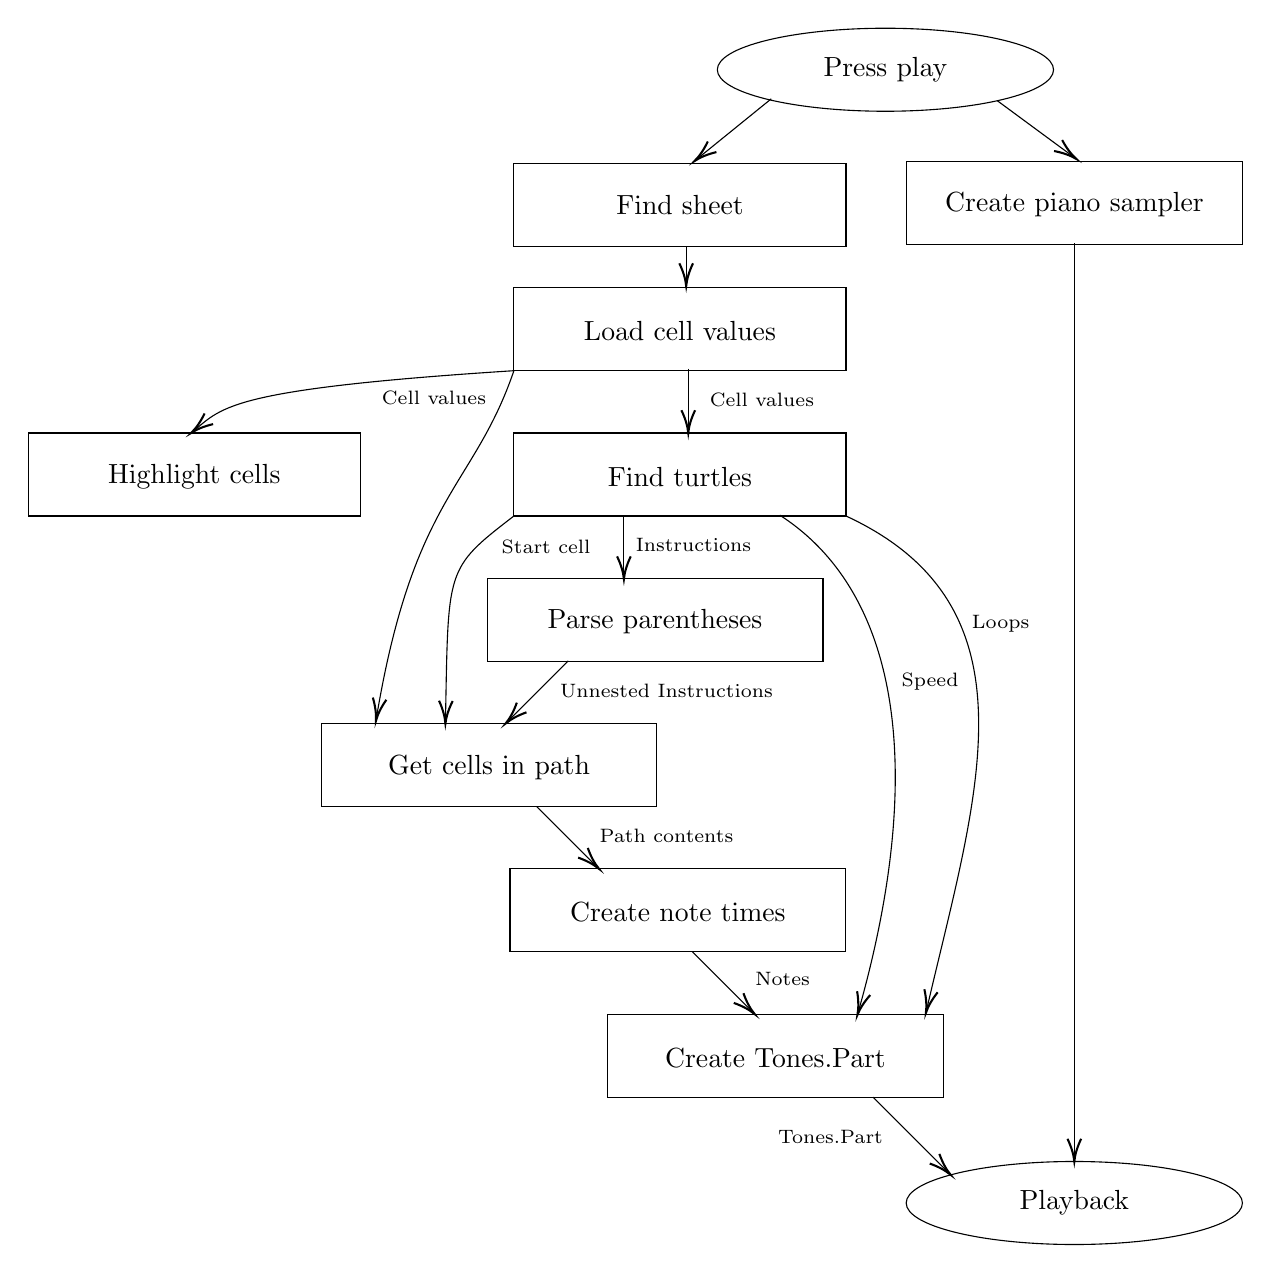
\begin{tikzpicture}[x=0.75pt,y=0.75pt,yscale=-1,xscale=1]
%uncomment if require: \path (0,604); %set diagram left start at 0, and has height of 604

%Shape: Rectangle [id:dp3390223975782729]
\draw   (244.5,71) -- (404.5,71) -- (404.5,111) -- (244.5,111) -- cycle ;

%Shape: Rectangle [id:dp7168559924493858]
\draw   (244.5,131) -- (404.5,131) -- (404.5,171) -- (244.5,171) -- cycle ;

%Shape: Rectangle [id:dp8835932361497658]
\draw   (433.7,70) -- (595.5,70) -- (595.5,110) -- (433.7,110) -- cycle ;

%Shape: Rectangle [id:dp9464422191216635]
\draw   (244.5,201) -- (404.5,201) -- (404.5,241) -- (244.5,241) -- cycle ;

%Shape: Rectangle [id:dp6384624480751633]
\draw   (231.6,271) -- (393.4,271) -- (393.4,311) -- (231.6,311) -- cycle ;

%Shape: Rectangle [id:dp2927464084046889]
\draw   (151.6,341) -- (313.4,341) -- (313.4,381) -- (151.6,381) -- cycle ;

%Shape: Rectangle [id:dp9052659554068596]
\draw   (242.6,411) -- (404.4,411) -- (404.4,451) -- (242.6,451) -- cycle ;

%Shape: Rectangle [id:dp5637329489183025]
\draw   (289.6,481) -- (451.4,481) -- (451.4,521) -- (289.6,521) -- cycle ;

%Curve Lines [id:da3917180624639185]
\draw    (244.5,241) .. controls (211.17,266.67) and (212.98,265.81) .. (211.52,339.88) ;
\draw [shift={(211.5,341)}, rotate = 271.14] [color={rgb, 255:red, 0; green, 0; blue, 0 }  ][line width=0.75]    (10.93,-3.29) .. controls (6.95,-1.4) and (3.31,-0.3) .. (0,0) .. controls (3.31,0.3) and (6.95,1.4) .. (10.93,3.29)   ;

%Straight Lines [id:da6961662223442007]
\draw    (297.5,241) -- (297.5,269.4) ;
\draw [shift={(297.5,271.4)}, rotate = 270] [color={rgb, 255:red, 0; green, 0; blue, 0 }  ][line width=0.75]    (10.93,-3.29) .. controls (6.95,-1.4) and (3.31,-0.3) .. (0,0) .. controls (3.31,0.3) and (6.95,1.4) .. (10.93,3.29)   ;

%Curve Lines [id:da9168950950169605]
\draw    (372.6,240.6) .. controls (431.31,278.41) and (442.88,365.52) .. (410.49,479.68) ;
\draw [shift={(410,481.4)}, rotate = 286.01] [color={rgb, 255:red, 0; green, 0; blue, 0 }  ][line width=0.75]    (10.93,-3.29) .. controls (6.95,-1.4) and (3.31,-0.3) .. (0,0) .. controls (3.31,0.3) and (6.95,1.4) .. (10.93,3.29)   ;

%Curve Lines [id:da7972588626438504]
\draw    (404.5,241) .. controls (499.03,284.78) and (467.32,375.49) .. (443.36,478.84) ;
\draw [shift={(443,480.4)}, rotate = 282.99] [color={rgb, 255:red, 0; green, 0; blue, 0 }  ][line width=0.75]    (10.93,-3.29) .. controls (6.95,-1.4) and (3.31,-0.3) .. (0,0) .. controls (3.31,0.3) and (6.95,1.4) .. (10.93,3.29)   ;

%Straight Lines [id:da6822022155717844]
\draw    (270.7,310.8) -- (241.91,339.59) ;
\draw [shift={(240.5,341)}, rotate = 315] [color={rgb, 255:red, 0; green, 0; blue, 0 }  ][line width=0.75]    (10.93,-3.29) .. controls (6.95,-1.4) and (3.31,-0.3) .. (0,0) .. controls (3.31,0.3) and (6.95,1.4) .. (10.93,3.29)   ;

%Straight Lines [id:da4884596231580207]
\draw    (255.5,381) -- (284.09,409.59) ;
\draw [shift={(285.5,411)}, rotate = 225] [color={rgb, 255:red, 0; green, 0; blue, 0 }  ][line width=0.75]    (10.93,-3.29) .. controls (6.95,-1.4) and (3.31,-0.3) .. (0,0) .. controls (3.31,0.3) and (6.95,1.4) .. (10.93,3.29)   ;

%Straight Lines [id:da9233366942734922]
\draw    (330.5,451) -- (359.09,479.59) ;
\draw [shift={(360.5,481)}, rotate = 225] [color={rgb, 255:red, 0; green, 0; blue, 0 }  ][line width=0.75]    (10.93,-3.29) .. controls (6.95,-1.4) and (3.31,-0.3) .. (0,0) .. controls (3.31,0.3) and (6.95,1.4) .. (10.93,3.29)   ;

%Straight Lines [id:da3670498457872964]
\draw    (417.5,521) -- (453.49,556.99) ;
\draw [shift={(454.9,558.4)}, rotate = 225] [color={rgb, 255:red, 0; green, 0; blue, 0 }  ][line width=0.75]    (10.93,-3.29) .. controls (6.95,-1.4) and (3.31,-0.3) .. (0,0) .. controls (3.31,0.3) and (6.95,1.4) .. (10.93,3.29)   ;

%Straight Lines [id:da28794703530347365]
\draw    (327.5,111) -- (327.5,128.2) ;
\draw [shift={(327.5,130.2)}, rotate = 270] [color={rgb, 255:red, 0; green, 0; blue, 0 }  ][line width=0.75]    (10.93,-3.29) .. controls (6.95,-1.4) and (3.31,-0.3) .. (0,0) .. controls (3.31,0.3) and (6.95,1.4) .. (10.93,3.29)   ;

%Straight Lines [id:da33376731250782754]
\draw    (328.5,170) -- (328.5,199) ;
\draw [shift={(328.5,201)}, rotate = 270] [color={rgb, 255:red, 0; green, 0; blue, 0 }  ][line width=0.75]    (10.93,-3.29) .. controls (6.95,-1.4) and (3.31,-0.3) .. (0,0) .. controls (3.31,0.3) and (6.95,1.4) .. (10.93,3.29)   ;

%Curve Lines [id:da2676626927985757]
\draw    (244.5,171) .. controls (225.1,227.72) and (196.29,230.77) .. (178.27,338.17) ;
\draw [shift={(178,339.8)}, rotate = 279.38] [color={rgb, 255:red, 0; green, 0; blue, 0 }  ][line width=0.75]    (10.93,-3.29) .. controls (6.95,-1.4) and (3.31,-0.3) .. (0,0) .. controls (3.31,0.3) and (6.95,1.4) .. (10.93,3.29)   ;

%Straight Lines [id:da024649031996502035]
\draw    (514.5,109.6) -- (514.5,550) ;
\draw [shift={(514.5,552)}, rotate = 270] [color={rgb, 255:red, 0; green, 0; blue, 0 }  ][line width=0.75]    (10.93,-3.29) .. controls (6.95,-1.4) and (3.31,-0.3) .. (0,0) .. controls (3.31,0.3) and (6.95,1.4) .. (10.93,3.29)   ;

%Shape: Ellipse [id:dp13505581605963868]
\draw   (433.5,572) .. controls (433.5,560.95) and (469.76,552) .. (514.5,552) .. controls (559.24,552) and (595.5,560.95) .. (595.5,572) .. controls (595.5,583.05) and (559.24,592) .. (514.5,592) .. controls (469.76,592) and (433.5,583.05) .. (433.5,572) -- cycle ;

%Shape: Ellipse [id:dp006287630832967794]
\draw   (342.5,26) .. controls (342.5,14.95) and (378.76,6) .. (423.5,6) .. controls (468.24,6) and (504.5,14.95) .. (504.5,26) .. controls (504.5,37.05) and (468.24,46) .. (423.5,46) .. controls (378.76,46) and (342.5,37.05) .. (342.5,26) -- cycle ;

%Straight Lines [id:da09048722077694915]
\draw    (368.5,40) -- (333.05,68.74) ;
\draw [shift={(331.5,70)}, rotate = 320.96000000000004] [color={rgb, 255:red, 0; green, 0; blue, 0 }  ][line width=0.75]    (10.93,-3.29) .. controls (6.95,-1.4) and (3.31,-0.3) .. (0,0) .. controls (3.31,0.3) and (6.95,1.4) .. (10.93,3.29)   ;

%Straight Lines [id:da9578993167654264]
\draw    (477.5,41) -- (513.89,67.81) ;
\draw [shift={(515.5,69)}, rotate = 216.38] [color={rgb, 255:red, 0; green, 0; blue, 0 }  ][line width=0.75]    (10.93,-3.29) .. controls (6.95,-1.4) and (3.31,-0.3) .. (0,0) .. controls (3.31,0.3) and (6.95,1.4) .. (10.93,3.29)   ;

%Shape: Rectangle [id:dp25073410390478523]
\draw   (10.5,201) -- (170.5,201) -- (170.5,241) -- (10.5,241) -- cycle ;

%Curve Lines [id:da2454539812308738]
\draw    (244.5,171) .. controls (108.92,179.69) and (104.17,188.37) .. (90.53,199.75) ;
\draw [shift={(89,201)}, rotate = 321.34000000000003] [color={rgb, 255:red, 0; green, 0; blue, 0 }  ][line width=0.75]    (10.93,-3.29) .. controls (6.95,-1.4) and (3.31,-0.3) .. (0,0) .. controls (3.31,0.3) and (6.95,1.4) .. (10.93,3.29)   ;


% Text Node
\draw (324.5,91) node  [align=left] {Find sheet};
% Text Node
\draw (324.5,152) node  [align=left] {Load cell values};
% Text Node
\draw (514.6,91) node  [align=left] {Create piano sampler};
% Text Node
\draw (324.5,222) node  [align=left] {Find turtles};
% Text Node
\draw (312.5,292) node  [align=left] {Parse parentheses};
% Text Node
\draw (232.5,362) node  [align=left] {Get cells in path};
% Text Node
\draw (323.5,432) node  [align=left] {Create note times};
% Text Node
\draw (370.5,502) node  [align=left] {Create Tones.Part};
% Text Node
\draw (514.5,572) node [] [align=left] {\textcolor[rgb]{0,0,0}{Playback}};
% Text Node
\draw (260,256) node  [align=left] {{\scriptsize Start cell}};
% Text Node
\draw (331,255) node  [align=left] {{\scriptsize Instructions}};
% Text Node
\draw (445,321) node  [align=left] {{\scriptsize Speed}};
% Text Node
\draw (479,293) node  [align=left] {{\scriptsize Loops}};
% Text Node
\draw (318,325) node  [align=left] {{\scriptsize Unnested Instructions}};
% Text Node
\draw (318,395) node  [align=left] {{\scriptsize Path contents}};
% Text Node
\draw (374,464) node  [align=left] {{\scriptsize Notes}};
% Text Node
\draw (397,540) node  [align=left] {{\scriptsize Tones.Part}};
% Text Node
\draw (206,184) node  [align=left] {{\scriptsize Cell values}};
% Text Node
\draw (423.5,26) node [] [align=left] {Press play};
% Text Node
\draw (364,185) node  [align=left] {{\scriptsize Cell values}};
% Text Node
\draw (90.5,222) node  [align=left] {Highlight cells};


\end{tikzpicture}

\end{center}

\begin{algorithm}[!htbp]
\caption{Parsing bracketed expression}\label{alg:parenthesis}
\begin{algorithmic}[1]
\Procedure{parseBrackets}{$str$}

   \State $idPadding\gets \texttt{\upquote{\_\_\_}}$
   \State $unnestedStr\gets []$
   \State $deepestLevelBracketsRE\gets \texttt{RegExp(\upquote{\textbackslash\textbackslash([\^{}\textbackslash\textbackslash(\textbackslash\textbackslash)]*\textbackslash\textbackslash)})}$
   \State $replacementIDRE\gets \texttt{RegExp(\upquote{\textbackslash\textbackslash} + }idPadding\texttt{ + \upquote{([0-9]+)} + }idPadding\texttt{)}$\\

   \Procedure{replaceDeepestBracket}{$x$}
     \State \texttt{unnestedStr.push(x.substring(1, x.length-1))}
     \State \texttt{\textbf{return} idPadding + (unnestedStr.length - 1) + idPadding}
   \EndProcedure \\

   \While{\texttt{deepestLevelBracketsRE.test(str)}}
     \State \texttt{str = str.replace(deepestLevelBracketsRE,replaceDeepestBracket)}
   \EndWhile

   \State \texttt{unnestedStr[0] = str}\\

   \Procedure{reNest}{$outerStr$}
     \State $renestingStr\gets []$
     \While{There is a match of $replacementIDRE$ in $outerStr$}
       \State $matchIndex\gets$ index of the match in $outerStr$
       \State $matchID\gets$ ID of the match (number between padding)
       \State $matchString\gets$ matched string\\

       \If{$matchIndex >$ 0}
				\State $renestingStr$.push($outestStr$.substring(0, $matchIndex$))
			\EndIf
			\State $renestingStr$.push(reNest($unnestedStr$[$firstMatchID$]))
			\State $outestStr$ = $outestStr$.substring($matchIndex$ + $matchString$.length)
     \EndWhile
     \State $renestingStr$.push($outestStr$)
     \State \textbf{return} $renestingStr$
   \EndProcedure \\

   \State \textbf{return} reNest($unnestedStr$[0])

\EndProcedure
\end{algorithmic}
\end{algorithm}

\section{Simple diagrams}

Simple diagrams can be written directly in \LaTeX.  For example, see
figure~\ref{latexpic1} on page~\pageref{latexpic1} and see
figure~\ref{latexpic2} on page~\pageref{latexpic2}.

\begin{figure}
\setlength{\unitlength}{1mm}
\begin{center}
\begin{picture}(125,100)
\put(0,80){\framebox(50,10){AAA}}
\put(0,60){\framebox(50,10){BBB}}
\put(0,40){\framebox(50,10){CCC}}
\put(0,20){\framebox(50,10){DDD}}
\put(0,00){\framebox(50,10){EEE}}

\put(75,80){\framebox(50,10){XXX}}
\put(75,60){\framebox(50,10){YYY}}
\put(75,40){\framebox(50,10){ZZZ}}

\put(25,80){\vector(0,-1){10}}
\put(25,60){\vector(0,-1){10}}
\put(25,50){\vector(0,1){10}}
\put(25,40){\vector(0,-1){10}}
\put(25,20){\vector(0,-1){10}}

\put(100,80){\vector(0,-1){10}}
\put(100,70){\vector(0,1){10}}
\put(100,60){\vector(0,-1){10}}
\put(100,50){\vector(0,1){10}}

\put(50,65){\vector(1,0){25}}
\put(75,65){\vector(-1,0){25}}
\end{picture}
\end{center}
\caption{A picture composed of boxes and vectors.}
\label{latexpic1}
\end{figure}

\begin{figure}
\setlength{\unitlength}{1mm}
\begin{center}

\begin{picture}(100,70)
\put(47,65){\circle{10}}
\put(45,64){abc}

\put(37,45){\circle{10}}
\put(37,51){\line(1,1){7}}
\put(35,44){def}

\put(57,25){\circle{10}}
\put(57,31){\line(-1,3){9}}
\put(57,31){\line(-3,2){15}}
\put(55,24){ghi}

\put(32,0){\framebox(10,10){A}}
\put(52,0){\framebox(10,10){B}}
\put(37,12){\line(0,1){26}}
\put(37,12){\line(2,1){15}}
\put(57,12){\line(0,2){6}}
\end{picture}

\end{center}
\caption{A diagram composed of circles, lines and boxes.}
\label{latexpic2}
\end{figure}



\section{Adding more complicated graphics}

The use of \LaTeX\ format can be tedious and it is often better to use
encapsulated postscript (EPS) or PDF to represent complicated graphics.
Figure~\ref{epsfig} and~\ref{xfig} on page \pageref{xfig} are
examples. The second figure was drawn using \texttt{xfig} and exported in
{\tt.eps} format. This is my recommended way of drawing all diagrams.


\begin{figure}[tbh]
\centerline{\includegraphics{figs/cuarms.pdf}}
\caption{Example figure using encapsulated postscript}
\label{epsfig}
\end{figure}

\begin{figure}[tbh]
\vspace{4in}
\caption{Example figure where a picture can be pasted in}
\label{pastedfig}
\end{figure}


\begin{figure}[tbh]
\centerline{\includegraphics{figs/diagram.pdf}}
\caption{Example diagram drawn using \texttt{xfig}}
\label{xfig}
\end{figure}


% TC:ignore

%%%%%%%%%%%%%%%%%%%%%%%%%%%%%%%%%%%%%%%%%%%%%%%%%%%%%%%%%%%%%%%%%%%%%
% the bibliography
\addcontentsline{toc}{chapter}{Bibliography}
\bibliography{refs}

%%%%%%%%%%%%%%%%%%%%%%%%%%%%%%%%%%%%%%%%%%%%%%%%%%%%%%%%%%%%%%%%%%%%%
% the appendices
\appendix

\chapter{Excello Implementation}

\section{bracketsParse.ts}
\label{appendix:parenthesis}
{\scriptsize\verbatiminput{chapters/implementation/parenthesis.ts}}

% \chapter{Project Proposal}

\includepdf[pages=-]{chapters/proposalAnon}

% TC:endignore

\end{document}
